% Options for packages loaded elsewhere
\PassOptionsToPackage{unicode}{hyperref}
\PassOptionsToPackage{hyphens}{url}
\PassOptionsToPackage{dvipsnames,svgnames,x11names}{xcolor}
%
\documentclass[
]{book}
\title{Décrire et inférer. Une introduction intuitive à l'analyse quantitative avec R}
\usepackage{etoolbox}
\makeatletter
\providecommand{\subtitle}[1]{% add subtitle to \maketitle
  \apptocmd{\@title}{\par {\large #1 \par}}{}{}
}
\makeatother
\subtitle{Notes de cours}
\author{Alexandre Blanchet\\
McGill University}
\date{mars 2018}

\usepackage{amsmath,amssymb}
\usepackage{lmodern}
\usepackage{iftex}
\ifPDFTeX
  \usepackage[T1]{fontenc}
  \usepackage[utf8]{inputenc}
  \usepackage{textcomp} % provide euro and other symbols
\else % if luatex or xetex
  \usepackage{unicode-math}
  \defaultfontfeatures{Scale=MatchLowercase}
  \defaultfontfeatures[\rmfamily]{Ligatures=TeX,Scale=1}
\fi
% Use upquote if available, for straight quotes in verbatim environments
\IfFileExists{upquote.sty}{\usepackage{upquote}}{}
\IfFileExists{microtype.sty}{% use microtype if available
  \usepackage[]{microtype}
  \UseMicrotypeSet[protrusion]{basicmath} % disable protrusion for tt fonts
}{}
\makeatletter
\@ifundefined{KOMAClassName}{% if non-KOMA class
  \IfFileExists{parskip.sty}{%
    \usepackage{parskip}
  }{% else
    \setlength{\parindent}{0pt}
    \setlength{\parskip}{6pt plus 2pt minus 1pt}}
}{% if KOMA class
  \KOMAoptions{parskip=half}}
\makeatother
\usepackage{xcolor}
\IfFileExists{xurl.sty}{\usepackage{xurl}}{} % add URL line breaks if available
\IfFileExists{bookmark.sty}{\usepackage{bookmark}}{\usepackage{hyperref}}
\hypersetup{
  pdftitle={Décrire et inférer. Une introduction intuitive à l'analyse quantitative avec R},
  colorlinks=true,
  linkcolor={Maroon},
  filecolor={Maroon},
  citecolor={Blue},
  urlcolor={blue},
  pdfcreator={LaTeX via pandoc}}
\urlstyle{same} % disable monospaced font for URLs
\usepackage{color}
\usepackage{fancyvrb}
\newcommand{\VerbBar}{|}
\newcommand{\VERB}{\Verb[commandchars=\\\{\}]}
\DefineVerbatimEnvironment{Highlighting}{Verbatim}{commandchars=\\\{\}}
% Add ',fontsize=\small' for more characters per line
\usepackage{framed}
\definecolor{shadecolor}{RGB}{248,248,248}
\newenvironment{Shaded}{\begin{snugshade}}{\end{snugshade}}
\newcommand{\AlertTok}[1]{\textcolor[rgb]{0.94,0.16,0.16}{#1}}
\newcommand{\AnnotationTok}[1]{\textcolor[rgb]{0.56,0.35,0.01}{\textbf{\textit{#1}}}}
\newcommand{\AttributeTok}[1]{\textcolor[rgb]{0.77,0.63,0.00}{#1}}
\newcommand{\BaseNTok}[1]{\textcolor[rgb]{0.00,0.00,0.81}{#1}}
\newcommand{\BuiltInTok}[1]{#1}
\newcommand{\CharTok}[1]{\textcolor[rgb]{0.31,0.60,0.02}{#1}}
\newcommand{\CommentTok}[1]{\textcolor[rgb]{0.56,0.35,0.01}{\textit{#1}}}
\newcommand{\CommentVarTok}[1]{\textcolor[rgb]{0.56,0.35,0.01}{\textbf{\textit{#1}}}}
\newcommand{\ConstantTok}[1]{\textcolor[rgb]{0.00,0.00,0.00}{#1}}
\newcommand{\ControlFlowTok}[1]{\textcolor[rgb]{0.13,0.29,0.53}{\textbf{#1}}}
\newcommand{\DataTypeTok}[1]{\textcolor[rgb]{0.13,0.29,0.53}{#1}}
\newcommand{\DecValTok}[1]{\textcolor[rgb]{0.00,0.00,0.81}{#1}}
\newcommand{\DocumentationTok}[1]{\textcolor[rgb]{0.56,0.35,0.01}{\textbf{\textit{#1}}}}
\newcommand{\ErrorTok}[1]{\textcolor[rgb]{0.64,0.00,0.00}{\textbf{#1}}}
\newcommand{\ExtensionTok}[1]{#1}
\newcommand{\FloatTok}[1]{\textcolor[rgb]{0.00,0.00,0.81}{#1}}
\newcommand{\FunctionTok}[1]{\textcolor[rgb]{0.00,0.00,0.00}{#1}}
\newcommand{\ImportTok}[1]{#1}
\newcommand{\InformationTok}[1]{\textcolor[rgb]{0.56,0.35,0.01}{\textbf{\textit{#1}}}}
\newcommand{\KeywordTok}[1]{\textcolor[rgb]{0.13,0.29,0.53}{\textbf{#1}}}
\newcommand{\NormalTok}[1]{#1}
\newcommand{\OperatorTok}[1]{\textcolor[rgb]{0.81,0.36,0.00}{\textbf{#1}}}
\newcommand{\OtherTok}[1]{\textcolor[rgb]{0.56,0.35,0.01}{#1}}
\newcommand{\PreprocessorTok}[1]{\textcolor[rgb]{0.56,0.35,0.01}{\textit{#1}}}
\newcommand{\RegionMarkerTok}[1]{#1}
\newcommand{\SpecialCharTok}[1]{\textcolor[rgb]{0.00,0.00,0.00}{#1}}
\newcommand{\SpecialStringTok}[1]{\textcolor[rgb]{0.31,0.60,0.02}{#1}}
\newcommand{\StringTok}[1]{\textcolor[rgb]{0.31,0.60,0.02}{#1}}
\newcommand{\VariableTok}[1]{\textcolor[rgb]{0.00,0.00,0.00}{#1}}
\newcommand{\VerbatimStringTok}[1]{\textcolor[rgb]{0.31,0.60,0.02}{#1}}
\newcommand{\WarningTok}[1]{\textcolor[rgb]{0.56,0.35,0.01}{\textbf{\textit{#1}}}}
\usepackage{longtable,booktabs,array}
\usepackage{calc} % for calculating minipage widths
% Correct order of tables after \paragraph or \subparagraph
\usepackage{etoolbox}
\makeatletter
\patchcmd\longtable{\par}{\if@noskipsec\mbox{}\fi\par}{}{}
\makeatother
% Allow footnotes in longtable head/foot
\IfFileExists{footnotehyper.sty}{\usepackage{footnotehyper}}{\usepackage{footnote}}
\makesavenoteenv{longtable}
\usepackage{graphicx}
\makeatletter
\def\maxwidth{\ifdim\Gin@nat@width>\linewidth\linewidth\else\Gin@nat@width\fi}
\def\maxheight{\ifdim\Gin@nat@height>\textheight\textheight\else\Gin@nat@height\fi}
\makeatother
% Scale images if necessary, so that they will not overflow the page
% margins by default, and it is still possible to overwrite the defaults
% using explicit options in \includegraphics[width, height, ...]{}
\setkeys{Gin}{width=\maxwidth,height=\maxheight,keepaspectratio}
% Set default figure placement to htbp
\makeatletter
\def\fps@figure{htbp}
\makeatother
\setlength{\emergencystretch}{3em} % prevent overfull lines
\providecommand{\tightlist}{%
  \setlength{\itemsep}{0pt}\setlength{\parskip}{0pt}}
\setcounter{secnumdepth}{5}
\usepackage{booktabs}
\ifLuaTeX
  \usepackage{selnolig}  % disable illegal ligatures
\fi
\usepackage[]{natbib}
\bibliographystyle{plainnat}

\begin{document}
\maketitle
\begin{abstract}
Ce document contient les notes de cours de mon enseignement de l'introduction aux statistiques. Il vise principalement les étudiants en science politique, mais pourrait aussi servir aux étudiants de tous les domaines qui utilisent les méthodes quantitatives. Les exemples utilisés sont cependant tirés de la vie politique. Le document couvre d'abord l'introduction à R et les manipulations de bases avec le logiciel. Une emphase particulière est ensuite portée sur la régression linéaire. Les autres types de régression, notamment les régressions logistiques et multinomiales, seront ajoutées éventuellement. Finalement, le document aborde les questions liées à l'inférence statistique. Tout le code R utilisé est reproduit dans ce document et est facilement reproductible. L'accent est mis sur la compréhension intuitive des méthodes statistiques elles-mêmes plutôt que sur l'aspect «computationnel» de leur mise en application. Cependant, cet aspect est vu en parallèle afin d'aider les lecteurs à saisir progressivement comment sont mises en application les méthodes statistiques abordées. Ce document est une version préliminaire et les commentaires et suggestions sont bienvenus! Je n'ai aucun problème à ce que ce matériel soit utilisé pour votre propre enseignement, en autant que les crédits me soient adéquatement attribués. Cette version est en date de mars 2018. Ces notes s'accompagnaient d'un enseignement en classe et des explications additionnelles sur le code R étaient souvent fournies. Ce document n'était pas initialement prévu pour être utilsé comme une source unique et l'approche de programmation ne suit donc pas toujours un paradigme cohérent. L'idée initiale était d'illustrer plusieurs manières de faire en fournissant les détails lors des séances en classe. Sachant que plusieurs enseignants utlisent ce document pour l'enseignement, j'entends progressivement améliorer cet aspect dans les prochains mois. J'en profiterai pour actualiser certaines techniques de programmation.
\end{abstract}

{
\hypersetup{linkcolor=}
\setcounter{tocdepth}{1}
\tableofcontents
}
\hypertarget{objectifs}{%
\chapter{Objectifs}\label{objectifs}}

L'objectif de ce document est d'abord de démystifier les approches statistiques. La plupart d'entre vous commencez votre maîtrise ou votre doctorat et aurez peut-être à apprendre une variété de méthodes statistiques pour mener à bien vos projets de recherche. Lorsque l'on commence à apprendre ces méthodes, il est facile d'être intimidé par des équations qui semblent bien complexes, ou par des logiciels qui peuvent de prime abord être difficiles à comprendre. Peut-être êtes-vous un peu plus avancé et avez déjà commencé à apprendre des méthodes plus complexes. Si c'est votre cas, cette séance vous sera utile aussi. Quand on commence à tenter de faire des choses plus complexes, il n'est pas rare que l'on se sente arriver en territoire inconnu et qu'on perde de vue l'objectif de base qui demeure pourtant simple.

Les statistiques ne sont pas de la magie et elles ne doivent jamais se substituer à votre jugement, étant entendu que celui-ci soit fondé sur une bonne compréhension de ce que les chiffres vous disent. Le fait que quelque chose soit «statistiquement significatif» ne constitue en aucun cas une sorte de sceau certifiant la véracité de ce que vous proposez. Quand on commence à faire des analyses statistiques, on est souvent obnubilé par les étoiles (ces fameuses étoiles, qui sont généralement le symbole associé à la significativité statistique). Il est excitant d'appuyer sur un bouton et de voir des étoiles apparaître à côté des chiffres. La chose entraîne une sorte de «boucle béhaviorale» : on appuie sur un bouton et on obtient une récompense. La plupart d'entre-nous y succombons. Je l'ai fait au début et je le vois très souvent chez mes collègues plus jeunes qui commencent.

La réalité est que tous les modèles statistiques, les simples comme les plus complexes, ont deux objectifs généraux : décrire et inférer. Nous voulons \emph{décrire} des données quelconques et, si nécessaire (ce qui est le cas la plupart du temps puisque nous utilisons souvent des échantillons) en \emph{inférer} quelque chose à une population plus large. En tout temps donc, gardez à l'esprit ces deux notions, parce que c'est systématiquement ce que toute forme de d'analyse statistique cherche à faire.

Nous utiliserons ici le \href{https://www.r-project.org}{logiciel R} qui est gratuit et de plus en plus utilisé en science politique. Je vous suggère aussi de télécharger \href{https://www.rstudio.com}{R Studio} qui est une interface très utile facilitant l'utilisation de R. Ceci étant, ce cours ne porte pas spécifiquement sur R. Je vais d'abord vous donner quelques notions de bases et expliquer la syntaxe au fur et à mesure pour que vous puissiez la comprendre, mais je ne me lancerai pas dans de grandes explications concernant le logiciel lui-même. La raison est tout simplement que nous n'apprenons rien sans avoir la \emph{motivation} de le faire. Dans le cas de R (et de tous les logiciels statistiques), il est donc tout à fait inutile de se concentrer sur son utilisation sans en même temps vous donner des idées sur ce que vous pourriez faire avec le logiciel.

L'apprentissage de la syntaxe (l'aspect «computationnel» des méthodes quantitatives), se fait forcément par la pratique et celle-ci vient de la nécessité. Nous apprenons à faire quelque chose parce que nous avons un objectif en tête. Je vous donnerai ici les bases pour vous aider à vous repérer au travers de l'aspect computationnel des méthodes statistiques, mais lorsque vous serez seul dans votre bureau, prêt à faire une certaine analyse, vous aurez forcément à chercher sur internet. C'est tout à fait normal.

Je me concentrerai donc à vous donner des éléments de bases de l'analyse statistique et, au passage, nous verrons comment les faire avec R. Vous verrez alors les deux éléments conjointement et, lentement mais sûrement, la logique derrière la syntaxe de R vous apparaîtra de plus en plus claire. L'objectif central demeure cependant que vous développiez une compréhension plus intuitive des méthodes statistiques que je vais vous présenter. L'apprentissage de la syntaxe est donc un objectif secondaire, mais parallèle. Il ne fait pas de sens d'apprendre à utilisr une syntaxe sans comprendre ce qu'elle fait, et il fait de moins en moins de sens d'apprendre des méthodes statistiques sans savoir comment les appliquer dans la pratique. Il reste que la compréhension des méthodes demeure la priorité, parce que c'est cette compréhension qui vous motivera à les appliquer dans vos recherches et surtout, c'est cette compréhension qui vous permettra de bien le faire.

Si R vous intéresse, vous pouvez consulter le site web de \href{http://www.statmethods.net/index.html}{Quick-R} qui contient toutes les informations nécessaires pour vous aider à démarrer et aller plus loin avec le logiciel. Ceci étant, toute la syntaxe nécessaire pour reproduire les analyses présentées ici est inclue dans le document dans des blocs ombragé et le résultat produit par R sera précédé de \#\# pour chaque ligne. Vous pourrez donc vous y référer au besoin et adapter la syntaxe pour mener vos propres analyses.

\hypertarget{les-logiciels}{%
\section{Les logiciels}\label{les-logiciels}}

Une syntaxe est une série de commandes que l'on demande à un logiciel d'effectuer. Certains logiciels mettent un accent particulier sur les menus déroulants (notamment SPSS), alors que d'autres offrent un bel équilibre en la possibilité d'utiliser une syntaxe complète et intuitive, tout en ayant accès à des menus déroulant pour les tâches les plus communes (Stata). Tous les logiciels ont besoin d'une forme ou d'une autre de syntaxe parce qu'il serait tout simplement impossible d'avoir des menus déroulants pour toutes les analyses statistiques existantes. À l'inverse, la syntaxe offre des possibilités infinies. R n'offre pas de menus déroulant, mais il a l'avantage d'être gratuit et aussi complet (et même plus complet) que les logiciels payants.

Le premier avantage de la syntaxe est qu'elle est reproductible. On peut donc «rouler» une syntaxe sur des données et répéter nos analyses antérieures sans altérer les données initiales. Dans un univers où la reproductibilité de la recherche est de plus en plus important, l'utilisation de la syntaxe deviendra rapidement impératif. Par ailleurs, même les logiciels qui offrent des menus déroulant fonctionnent aussi à base de syntaxe afin que l'utilisateur puisse répéter facilement ses analyses au besoin et, comme mentionné plus haut, parce qu'il est impossible d'inclure en menus déroulant toutes les analyses statistiques possibles.

À mon avis, SPSS devrait être laissé de côté par quiconque commence à utiliser des méthodes quantitaves. Il s'agit d'un bon logiciel, mais il a été créé il y a très longtemps et pour cette raison, sa syntaxe n'a jamais réellement été conçue pour être utilisée directement. En conséquence, le langage syntaxique de SPSS est réellement pénible à utiliser. Par ailleurs, SPSS est incroyablement dispendieux.

Stata est un excelent logiciel et sa syntaxe est très complète et intuitive. Stata a aussi de bons menus déroulants qui peuvent être très utiles pour nous apprendre à utiliser la syntaxe puisque l'on peut faire une analyse d'abord en utilisant le menu déroulant, puis regarder la syntaxe produite par Stata. Il faut cependant payer la licence pour l'utiliser (entre 400\$ à 1000\$ suivant la version et le statut professionnel), ou ne l'utiliser que sur les postes informatiques disponibles dans les laboratoires universitaires.

R est aussi puissant que Stata (voir plus), et il est gratuit. Par ailleurs, il y a une très grande communeauté d'utilisateurs de R et il existe donc beaucoup de «packages» qu'il est possible de télécharger gratuitement pour ajouter des fonctions à R (Stata offre aussi cette possibilité, mais il y en a beaucoup moins). En conséquence, R est toujours en avance sur Stata et il permet de faire des analyses qui n'ont pas forcément encore été implémentées dans Stata. Le seul désavantage de R par rapport à Stata est que sa syntaxe est un peu plus difficile à apprendre, mais une fois qu'on la maîtrise, il n'y a vraiment plus aucune raison de s'ennuyer Stata.

Au final, l'apprentissage de n'importe quel logiciel implique forcément beaucoup d'essais-erreurs et des consultations fréquentes de notre ami Google. Stata est un peu plus facile à apprendre, mais puisqu'il faut apprendre un nouveau logiciel, aussi bien fournir le petit effort supplémentaire pour apprendre R qui est aussi complet, plus souple, gratuit, et qui offre une communeauté d'utilisateurs très réactive.

Nous pourrions continuer à voir séparément différentes fonctions de R, mais cela deviendrait vite interminable. Vous devriez maintenant avoir les bases pour saisir la logique de la syntaxe de R et pour avoir une idée générale de ce qu'est une syntaxe. C'est ce qui est important. Il est impossible de couvrir le fonctionnement de R sans aussi apprendre à faire des statistiques. Si vous décidez d'apprendre R, vous devrez de toute manière apprendre par essai-erreur et cela viendra avec la pratique. Google sera votre plus grand ami!

Tournons-nous maintenant sur l'objectif principal de toute analyse statistique : décrire.

\hypertarget{introduction-guxe9nuxe9rale-uxe0-r}{%
\chapter{Introduction générale à R}\label{introduction-guxe9nuxe9rale-uxe0-r}}

Le \href{https://www.r-project.org}{logiciel R} est gratuit et très puissant. Il est littéralement possible de faire toutes les analyses statistiques imaginables avec R, et cela est notamment dû au fait qu'il y a une très large communauté d'utilisateurs de R qui produisent des «packages» qui ajoutent des fonctions au logiciel. Le désavantage de R est que la courbe d'apprentissage est plus difficile qu'avec d'autres logiciels parce que R n'offre pas de menus déroulants. Cependant \emph{après} avoir \href{https://www.r-project.org}{installé R} sur votre ordinateur, il est possible d'installer \href{https://www.rstudio.com}{R Studio} qui est aussi gratuit.R Studio n'est pas un logiciel qui fonctionne seul, il nécessite que la base de R soit installée sur votre ordinateur. R Studio est une interface qui va «par-dessus» R et facilite un peu son utilisation. Il faut donc préalablement avoir installé R, puis on installe R Studio. Une fois cela fait, on peut utiliser R Studio.

R Studio propose par défaut quatre panels qui peuvent être positionnés à votre guise dans les préférences du logiciel. Si vous ne modifiez pas les préférences, le panel où nous écrivons la syntaxe est en haut à gauche. Sous ce panel, en bas à gauche, se trouve la «console» de R, qui renvoie les résultats des commandes que nous passons à R via notre syntaxe. En haut à droite se trouve le panel «Environnement» qui liste tous les objets chargé en mémoire dans R. En bas à droite se trouve le panel des fichiers, figures, packages (et autres) où seront affichés les figures et où nous pourront charger et installer des packages.

\hypertarget{les-packages}{%
\section{Les packages}\label{les-packages}}

R vient par défaut avec une série de commandes très utiles, mais il existe aussi beaucoup de «packages» qui ajoutent des fonctions au logiciel. Les packages doivent être installés sur votre ordinateur (et souvent ré-installés lorsque vous mettez à jour votre version de R), mais ensuite vous n'avez pas à les installer de nouveau. Cependant, si vous désirez utiliser les fonctions d'un package, il faut systématiquement le charger dans votre session R. R fonctionne ainsi parce que si tous les packages installés sur votre ordinateurs étaient systématiquement actifs sans avoir à les charger, R deviendrait de plus en plus lourd et lent parce qu'il exigerait énormément de mémoire RAM. Donc, on \emph{installe} d'abord un package quand on veut pouvoir utiliser ses fonctions. Cette installation ne se fait qu'une seule fois (ou lors des mises à jour), mais ensuite on doit \emph{charger} à chaque session les packages que l'on veut utiliser.

Par exemple, le package \emph{ggplot2} est très utilie pour faire des graphiques. Si je ne l'ai jamais installé sur mon ordinateur, je peux le faire en cliquant sur l'onglet «packages» du panel en bas à droite, puis «install», puis je peux taper le nom du package (``ggplot2'') dans le menu. R Studio cherchera la package correspondant dans la banque de package accessible via internet. En cliaquant sur install, R Studio installera le package. Alternativement, on peut aussi procéder directement par la syntaxe comme suit avec la commande ``install.packages(''NOM DU PACKAGE'')``, donc dans notre cas \emph{install.packages(``ggplot2'')}.

Une fois que le package est installé, il apparaîtra dans la liste «System Library» sous l'onglet «package» du panel en bas à droite. On peut simplement cliquer sur la case correspondant au package souhaité pour l'activer, ou encore mieux le faire via la syntaxe comme ceci :

\begin{Shaded}
\begin{Highlighting}[]
\FunctionTok{library}\NormalTok{(}\StringTok{"ggplot2"}\NormalTok{)}
\end{Highlighting}
\end{Shaded}

Notez que vous ne pouvez pas utiliser les fonctions d'un package s'il n'est pas chargé dans votre session. Pour cette raison, si vous écrivez un script qui utilise des fonctions qui viennent de certains packages, la bonne pratique est de charger ceux-ci dans votre syntaxe elle-même avant d'utiliser les fonctions. Autrement, vous aurez un message d'erreur et votre script ne pourra pas rouler du début à la fin. Il peut donc être pratique au début d'utiliser les menus et les cases cliquables, mais \emph{je vous suggère fortement} de copier et coller les lignes de code produites par ces actions dans votre syntaxe elle-même afin que vous contruisiez progressivement un script qui pourra ensuite être roulé du début à la fin sans erreurs. Une bonne méthode de travail et des syntaxes «propres» vous sauverons beaucoup de temps.

\hypertarget{le-working-directory}{%
\section{Le «working directory»}\label{le-working-directory}}

Comme tous les logiciels statistiques, R a en mémoire un endroit sur votre ordinateur qui est le «working directory». C'est à cet endroit que R placera par défaut tout ce que vous sauvegarderez durant votre session. Par défaut, R utilisera le dernier working directory qu'il a en méoire. Vous pouvez à tout moment changer le working directory comme ceci :

\begin{Shaded}
\begin{Highlighting}[]
\CommentTok{\#setwd("/output") \# setwd() pour set working directory}
\CommentTok{\# puis on place le lien vers le fichier souhaité dans la parenthèse. }
\end{Highlighting}
\end{Shaded}

On peut passer «par-dessus» le working directory en mémoire à un moment donné en référant au lien complet vers un fichier que l'on souhaite utiliser (ou dans lequel on souhaite sauvegarder quelque chose), mais l'avantage d'établir le working directory approprié est que R assumera alors que ce à quoi vous référez s'y trouve. Il est alors possible d'utiliser seulement le nom du fichier auquel on réfère (plutôt que le lien complet vers celui-ci). Il est donc de bonne pratique d'établir au début d'une syntaxe le working directory que vous souhaitez utiliser. Cela vous évitera d'avoir à écrire constement les liens complets vers les fichiers sur votre ordinateur.

\hypertarget{quelques-manipulations-initiales-avec-r}{%
\section{Quelques manipulations initiales avec R}\label{quelques-manipulations-initiales-avec-r}}

Pour vous aider à mieux saisir ce que nous ferons durant le cours et pour que vous ayez un petit guide de référence lorsque vous serez seul à votre bureau, je vais ici procéder à quelques manipulations de bases avec R. La syntaxe (ou les commandes) apparaîtront dans des blocs ombragé et le résultat produit par R apparaîtra sous ces blocs sur des lignes précédés de deux dièzes. Les annotations \emph{à l'intérieur} de la syntaxe seront précédées d'un seul dièse. Cela est nécessaire afin que R sache qu'il s'agit d'une annotation et non pas de commandes qu'il doit exécuter.

Commençons doucement en demandant à R de renvoyer le chiffre \(\pi\).

\begin{Shaded}
\begin{Highlighting}[]
\CommentTok{\# Ceci est une autre annonation. Nous allons entrer la commande "pi"}
\NormalTok{pi }\CommentTok{\# Ceci est une autre annotation que je place à côté de la commande.}
\end{Highlighting}
\end{Shaded}

\begin{verbatim}
## [1] 3.141593
\end{verbatim}

La commande «pi» est la ligne de commande et R nous renvoie le résultat sous le bloc ombragé sur la ligne précédée par deux dièses. Nous pourrions aussi demander à R de nous renvoyer toutes les couleurs qu'il a en mémoire. R contient par défaut 657 couleurs dans l'objet \emph{colors()} qui sont utilisées notamment pour faire les graphiques. Or, puisqu'il y en a 657, nous allons simplement lui demander de nous donner seulement les premières en utilisant la commande \emph{head()}, et en insérant \emph{colors()} dans la parenthèse de la commande \emph{head()} :

\begin{Shaded}
\begin{Highlighting}[]
\FunctionTok{head}\NormalTok{(}\FunctionTok{colors}\NormalTok{())}
\end{Highlighting}
\end{Shaded}

\begin{verbatim}
## [1] "white"         "aliceblue"     "antiquewhite"  "antiquewhite1"
## [5] "antiquewhite2" "antiquewhite3"
\end{verbatim}

Ici, le premier élément contenu dans l'objet \emph{colors()} est ``white'', le cinquième élément est ``antiquewhite2'' et le sixième ``antiquewhite3''. Si nous n'avions pas inséré \emph{colors()} à l'intérieur de la commande \emph{head()}, R nous aurait renvoyé la liste complète des 657 couleurs, ce qui aurait été interminable.

Nous pouvons aussi créer des objets qui peuvent contenir tout ce que l'on veut. Nous pouvons nommer ces objets de n'importe quelle manière. Créons ici l'objet «fadeldwill» qui contiendra la valeur de 1 :

\begin{Shaded}
\begin{Highlighting}[]
\NormalTok{fadeldwill }\OtherTok{\textless{}{-}} \DecValTok{1}
\end{Highlighting}
\end{Shaded}

Nous avons ici créé l'objet \emph{fadeldwill} et nous lui avons assigné la valeur de 1. Le signe \texttt{\textless{}-} est équivalent à =, ou peut être lu comme «insère ce qui est à droite dans l'objet à gauche de la flèche». L'objet \emph{fadeldwill} est maintenant en mémoire, mais R ne renvoie rien parce que nous ne lui avons pas demandé. Faisons-le.

\begin{Shaded}
\begin{Highlighting}[]
\NormalTok{fadeldwill}
\end{Highlighting}
\end{Shaded}

\begin{verbatim}
## [1] 1
\end{verbatim}

Nous voyons que \emph{fadeldwill} ne contient qu'un seul élément ({[}1{]}) qui est la valeur 1.

Nous pourrions changer le contenu de \emph{fadeldwill} pour ``abc'' au lieu de 1. Notez que je commence ici à annoter le contenu de la syntaxe en faisant précéder toute annotation d'un dièse afin que R sache qu'il ne s'agit pas de code qu'il doit exécuter. Les annotations sont très utiles pour clarifier une syntaxe et mieux s'y retrouver plus tard. Pour ceux qui sont familiers avec Stata, c'est l'équivalent de mettre une étoile (*) dans la syntaxe.

\begin{Shaded}
\begin{Highlighting}[]
\NormalTok{fadeldwill }\OtherTok{\textless{}{-}} \StringTok{"abc"} \CommentTok{\# Pour mettre abc dans fadeldwill. }
\CommentTok{\# Les guillements sont nécessaires puisque abc n\textquotesingle{}est pas numérique.}
\NormalTok{fadeldwill }\CommentTok{\# Pour demander à R de nous dire ce que contient fadeldwill.}
\end{Highlighting}
\end{Shaded}

\begin{verbatim}
## [1] "abc"
\end{verbatim}

Nous pourrions vouloir que \emph{fadeldwill} contienne plutôt une série de chiffres (disons : 1, 2, 3, 4, 5). Il faudra alors utiliser la fonction \emph{c()}, «c» pour «concatenate», et on insère ce que l'on veut dans la parenthèse, avec des virgules entres les éléments.

\begin{Shaded}
\begin{Highlighting}[]
\NormalTok{fadeldwill }\OtherTok{\textless{}{-}} \FunctionTok{c}\NormalTok{(}\DecValTok{1}\NormalTok{, }\DecValTok{2}\NormalTok{, }\DecValTok{3}\NormalTok{, }\DecValTok{4}\NormalTok{, }\DecValTok{5}\NormalTok{) }
\NormalTok{fadeldwill}
\end{Highlighting}
\end{Shaded}

\begin{verbatim}
## [1] 1 2 3 4 5
\end{verbatim}

Nous pourrions aussi vouloir mettre autre chose que des nombres dans \emph{fadeldwill} :

\begin{Shaded}
\begin{Highlighting}[]
\NormalTok{fadeldwill }\OtherTok{\textless{}{-}} \FunctionTok{c}\NormalTok{(}\StringTok{"A"}\NormalTok{, }\StringTok{"B"}\NormalTok{, }\StringTok{"C"}\NormalTok{, }\StringTok{"D"}\NormalTok{, }\StringTok{"E"}\NormalTok{) }
\NormalTok{fadeldwill}
\end{Highlighting}
\end{Shaded}

\begin{verbatim}
## [1] "A" "B" "C" "D" "E"
\end{verbatim}

Jusqu'à présent, nous avons systématiquement \emph{remplacé} le contenu de \emph{fadeldwill} par du nouveau contenu. Nous pourrions cependant vouloir lui \emph{ajouter} un nouvel élément à ce qu'il contient déjà. Ajoutons la lettre F à la suite de lettres que contient \emph{fadeldwill} :

\begin{Shaded}
\begin{Highlighting}[]
\NormalTok{fadeldwill }\OtherTok{\textless{}{-}} \FunctionTok{c}\NormalTok{(fadeldwill, }\StringTok{"F"}\NormalTok{) }\CommentTok{\# Ici, nous disons simplement que l\textquotesingle{}objet }
\CommentTok{\# fadeldwill contient fadeldwill et la lettre F. Donc, ce qu\textquotesingle{}était déjà }
\CommentTok{\# l\textquotesingle{}objet fadeldwill (soit "A", "B", "C", "D", "E") et on y ajoute F.}
\NormalTok{fadeldwill }
\end{Highlighting}
\end{Shaded}

\begin{verbatim}
## [1] "A" "B" "C" "D" "E" "F"
\end{verbatim}

Nous pourrions aussi vouloir \emph{retirer} un élément de \emph{fadeldwill}. Disons que nous voulions retirer C :

\begin{Shaded}
\begin{Highlighting}[]
\NormalTok{fadeldwill }\OtherTok{\textless{}{-}}\NormalTok{ fadeldwill[}\SpecialCharTok{{-}}\DecValTok{3}\NormalTok{] }\CommentTok{\# Nous voulons que fadeldwill demeure identique}
\CommentTok{\# mais en excluant "C", qui est la troisième valeur, d\textquotesingle{}où le [{-}3].}
\NormalTok{fadeldwill }
\end{Highlighting}
\end{Shaded}

\begin{verbatim}
## [1] "A" "B" "D" "E" "F"
\end{verbatim}

Nous aurions aussi pu vouloir retirer A et F :

\begin{Shaded}
\begin{Highlighting}[]
\NormalTok{fadeldwill }\OtherTok{\textless{}{-}}\NormalTok{ fadeldwill[}\SpecialCharTok{{-}}\FunctionTok{c}\NormalTok{(}\DecValTok{1}\NormalTok{, }\DecValTok{5}\NormalTok{)] }\CommentTok{\# Nous retirons le premier (A) et le }
\CommentTok{\# cinquième élément (F, devenu cinquième après le retrait de C).}
\CommentTok{\# Nous devons les mettre dans un c() parce qu\textquotesingle{}il y a plus d\textquotesingle{}un élément}
\CommentTok{\# à retirer}
\NormalTok{fadeldwill }
\end{Highlighting}
\end{Shaded}

\begin{verbatim}
## [1] "B" "D" "E"
\end{verbatim}

Nous pourrions aussi vouloir que R nous renvoie seulement le deuxième élément contenu dans \emph{fadeldwill} :

\begin{Shaded}
\begin{Highlighting}[]
\NormalTok{fadeldwill[}\DecValTok{2}\NormalTok{] }\CommentTok{\# Nous demandons à R de donner le 2e élément de fadeldwill}
\end{Highlighting}
\end{Shaded}

\begin{verbatim}
## [1] "D"
\end{verbatim}

R nous renvoie bien la lettre D, qui est maintenant le deuxième élément dans notre objet.

Nous pourrions aussi vouloir créer l'objet \emph{fadeldwillidou} qui contiendrait seulement le premier et le troisième élément de fadeldwill :

\begin{Shaded}
\begin{Highlighting}[]
\NormalTok{fadeldwillidou }\OtherTok{\textless{}{-}}\NormalTok{ fadeldwill[}\FunctionTok{c}\NormalTok{(}\DecValTok{1}\NormalTok{, }\DecValTok{3}\NormalTok{)]}
\NormalTok{fadeldwillidou}
\end{Highlighting}
\end{Shaded}

\begin{verbatim}
## [1] "B" "E"
\end{verbatim}

Encore une fois, si on veut \emph{ajouter} quelque chose à un objet qui existe déjà, il faut que l'objet lui-même soit inclu à droite de la flèche. Par exemple, si nous voulons ajouter A à \emph{fadeldwillidou} qui contient déjà B, E, il faut impérativement inclure \emph{fadeldwillidou} dans la parenthèse \emph{c()} à droite de la flèche.

\begin{Shaded}
\begin{Highlighting}[]
\NormalTok{fadeldwillidou }\OtherTok{\textless{}{-}} \FunctionTok{c}\NormalTok{(fadeldwillidou, }\StringTok{"A"}\NormalTok{)}
\end{Highlighting}
\end{Shaded}

Si l'on inclut pas l'objet lui-même à droite de la flèche, alors son contenu sera remplacé par ce qui est à droite de la flèche, sans préserver le contenu préalable. Par exemple, ici nous remplaçons complètement le contenu de \emph{fadeldwillidou} (B, E, A) par les nombres de 1 à 10.

\begin{Shaded}
\begin{Highlighting}[]
\NormalTok{fadeldwillidou }\OtherTok{\textless{}{-}} \FunctionTok{c}\NormalTok{(}\DecValTok{1}\NormalTok{,}\DecValTok{2}\NormalTok{,}\DecValTok{3}\NormalTok{,}\DecValTok{4}\NormalTok{,}\DecValTok{5}\NormalTok{,}\DecValTok{6}\NormalTok{,}\DecValTok{7}\NormalTok{,}\DecValTok{8}\NormalTok{,}\DecValTok{9}\NormalTok{,}\DecValTok{10}\NormalTok{)}
\NormalTok{fadeldwillidou}
\end{Highlighting}
\end{Shaded}

\begin{verbatim}
##  [1]  1  2  3  4  5  6  7  8  9 10
\end{verbatim}

Pour le meilleur et (surtout) pour le pire, le recodage est très certainement ce qui demande souvent le plus de travail lorsque nous faisons des analyses statistiques. Souvent, les variables ne sont pas codées comme on voudrait qu'elles le soient, ou il faut «nettoyer» les données brutes de sorte à les rendre analysables. Nous verrons cela plus en profondeur un peu plus loin, mais pour l'instant, voici quelques manipulations usuelles qu'il vous sera utile de comprendre.

Nous avons l'objet \emph{fadeldwill} qui contient B, D, E. Imaginons que nous voulions remplacer E par Z. Nous pouvons le faire comme ceci.

\begin{Shaded}
\begin{Highlighting}[]
\NormalTok{fadeldwill}
\end{Highlighting}
\end{Shaded}

\begin{verbatim}
## [1] "B" "D" "E"
\end{verbatim}

\begin{Shaded}
\begin{Highlighting}[]
\NormalTok{fadeldwill[fadeldwill }\SpecialCharTok{==} \StringTok{"E"}\NormalTok{] }\OtherTok{\textless{}{-}} \StringTok{"Z"}
\CommentTok{\# Remplace les valeurs de fadeldwillidou qui sont égales à "E" }
\CommentTok{\# et remplace les par "Z".}
\NormalTok{fadeldwill}
\end{Highlighting}
\end{Shaded}

\begin{verbatim}
## [1] "B" "D" "Z"
\end{verbatim}

Nous pourrions maintenant vouloir changer les valeurs de certains chiffres de \emph{fadeldwillidou} qui contient 1, 2, 3, 4, 5, 6, 7, 8, 9, 10. Disons que nous veulons que 2 soit remplacé par 1.

\begin{Shaded}
\begin{Highlighting}[]
\NormalTok{fadeldwillidou[fadeldwillidou }\SpecialCharTok{==} \DecValTok{2}\NormalTok{] }\OtherTok{\textless{}{-}} \DecValTok{1}
\CommentTok{\# Remplace les valeurs de fadeldwillidou qui sont égales à 2 }
\CommentTok{\# et remplace les par 1.}
\NormalTok{fadeldwillidou}
\end{Highlighting}
\end{Shaded}

\begin{verbatim}
##  [1]  1  1  3  4  5  6  7  8  9 10
\end{verbatim}

Imaginons maintenant que nous voulions que les chiffres de 3 à 7 soient remplacés par 4.

\begin{Shaded}
\begin{Highlighting}[]
\NormalTok{fadeldwillidou[fadeldwillidou }\SpecialCharTok{\textgreater{}} \DecValTok{2} \SpecialCharTok{\&}\NormalTok{ fadeldwillidou }\SpecialCharTok{\textless{}=}\DecValTok{7}\NormalTok{] }\OtherTok{\textless{}{-}} \DecValTok{4}
\CommentTok{\# Recode les valeurs de fadeldwillidou plus grandes que 2 et inférieure}
\CommentTok{\# ou égale à 7 et remplace par 4.}
\NormalTok{fadeldwillidou}
\end{Highlighting}
\end{Shaded}

\begin{verbatim}
##  [1]  1  1  4  4  4  4  4  8  9 10
\end{verbatim}

Nous pourrions aussi vouloir changer la valeur de 9 pour celle de 10

\begin{Shaded}
\begin{Highlighting}[]
\NormalTok{fadeldwillidou[fadeldwillidou }\SpecialCharTok{\textgreater{}} \DecValTok{8}\NormalTok{] }\OtherTok{\textless{}{-}} \DecValTok{10} \CommentTok{\# Recode les chiffres plus grand }
\CommentTok{\# que 8 pour qu\textquotesingle{}ils prennent la valeur de 10. }
\NormalTok{fadeldwillidou}
\end{Highlighting}
\end{Shaded}

\begin{verbatim}
##  [1]  1  1  4  4  4  4  4  8 10 10
\end{verbatim}

\begin{Shaded}
\begin{Highlighting}[]
\CommentTok{\# alternativement, dans ce cas nous aurions aussi pu faire }
\CommentTok{\# fadeldwillidou[fadeldwillidou == 9] \textless{}{-} 10}
\end{Highlighting}
\end{Shaded}

Dans la vraie vie, ces chiffres pourraient correspondre à des codes pour, par exemple, la couleur des yeux. 1 pourrait vouloir dire qu'une personne a les yeux bleus, 4 qu'elle a les yeux bruns, 8 qu'elle a les yeux pairs et 10 qu'elle a les yeux verts. Sachant cela, nous pourrions préférer avoir les labels plutôt que les chiffres. Cela pourrait être pratique plus tard.

\begin{Shaded}
\begin{Highlighting}[]
\NormalTok{fadeldwillidou }\OtherTok{\textless{}{-}} \FunctionTok{factor}\NormalTok{(fadeldwillidou, }
                          \AttributeTok{labels =} \FunctionTok{c}\NormalTok{(}\StringTok{"Bleus"}\NormalTok{, }\StringTok{"Bruns"}\NormalTok{, }
                                     \StringTok{"Pairs"}\NormalTok{, }\StringTok{"Verts"}\NormalTok{))}

\NormalTok{fadeldwillidou}
\end{Highlighting}
\end{Shaded}

\begin{verbatim}
##  [1] Bleus Bleus Bruns Bruns Bruns Bruns Bruns Pairs Verts Verts
## Levels: Bleus Bruns Pairs Verts
\end{verbatim}

\begin{Shaded}
\begin{Highlighting}[]
\FunctionTok{summary}\NormalTok{(fadeldwillidou)}
\end{Highlighting}
\end{Shaded}

\begin{verbatim}
## Bleus Bruns Pairs Verts 
##     2     5     1     2
\end{verbatim}

Les objets \emph{fadeldwill} et \emph{fadeldwillidou} sont en mémoire dans notre environnement de travail (workspace). Nous pouvons voir le contenu de tous les objets qui se trouvent dans cet environnement en faisant la commande \emph{objects()} :

\begin{Shaded}
\begin{Highlighting}[]
\FunctionTok{objects}\NormalTok{()}
\end{Highlighting}
\end{Shaded}

\begin{verbatim}
## [1] "fadeldwill"     "fadeldwillidou"
\end{verbatim}

Nous voyons que notre espace de travail ne contient pour l'instant que nos deux objets. Il y a \emph{fadeldwill} et \emph{fadeldwillidou}. R Studio nous permet de facilement voir tout le contenu de l'espace de travail sans passer de commande R en observant simplement le panel approprié dans l'interface.

L'espace de travail peut contenir une très grande quantité d'objets. Ceux-ci peuvent être des trivialités (comme c'est le cas ici), ou encore des choses plus importantes comme des bases de données (des matrices). Contrairement aux autres logiciels statistiques, il est donc très facile d'utiliser en même temps plusieurs bases de données avec R, ce qui est parfois très pratique et impossible (ou souvent fastidieux) avec les autres logiciels.

Ceci étant, puisque les objets \emph{fadeldwill} et \emph{fadeldwillidou} nous seront complètement inutiles, il vaut aussi bien les effacer :

\begin{Shaded}
\begin{Highlighting}[]
\FunctionTok{rm}\NormalTok{(fadeldwill, fadeldwillidou) }\CommentTok{\# rm() pour "remove". Nous n\textquotesingle{}avons pas besoin}
\CommentTok{\# de mettre fadeldwill et fadeldwillidou à l\textquotesingle{}intérieur d\textquotesingle{}un c() parce que}
\CommentTok{\# la commande rm() implique forcément une liste d\textquotesingle{}un ou plusieurs éléments}
\CommentTok{\# et rien d\textquotesingle{}autre. Alternativement, nous pourrions faire rm(list = ls())}
\CommentTok{\# pour vider complètement l\textquotesingle{}espace de travail.}

\FunctionTok{objects}\NormalTok{() }\CommentTok{\# objects() est maintenant vide.}
\end{Highlighting}
\end{Shaded}

\begin{verbatim}
## character(0)
\end{verbatim}

\hypertarget{une-syntaxe-qui-roule-une-bonne-muxe9thode-de-travail}{%
\section{Une syntaxe qui roule : une bonne méthode de travail}\label{une-syntaxe-qui-roule-une-bonne-muxe9thode-de-travail}}

Il est possible d'écrire directement des commandes dans la console de R et dans certains cas cela peut être utile, mais il est beaucoup mieux d'écrire vos commandes dans un script qui pourra ensuite être réutilisé. Par ailleurs, un bon script doit pouvoir être roulé du début à la fin sans erreur. Des erreurs dans un script surviendront, par exemple, si à un moment donné dans la série de commandes on fait référence à un objet qui n'a pas préalablement été créé dans le script lui-même.

Imaginons que j'utilise la console pour créer l'objet x qui contiendra la lettre A. J'écrirais donc la commande suivante directement dans la console plutôt que dans un script :

\begin{Shaded}
\begin{Highlighting}[]
\NormalTok{x }\OtherTok{\textless{}{-}} \StringTok{"A"}
\end{Highlighting}
\end{Shaded}

Je viens de créer l'objet \emph{x}, il existe en ce moment dans ma session, mais je ne l'ai pas fait en écrivant la commande dans un scrip. Ensuite, dans un fichier de synataxe, je modifie l'objet \emph{x} pour inclure aussi ``B''. J'écris donc la commande suivante dans un fichier de syntaxe:

\begin{Shaded}
\begin{Highlighting}[]
\NormalTok{x }\OtherTok{\textless{}{-}} \FunctionTok{c}\NormalTok{(x, }\StringTok{"B"}\NormalTok{)}
\end{Highlighting}
\end{Shaded}

Remarquez cependant que notre objet \emph{x} a d'abord été créé directement dans la console et contenait la lettre A, puis nous l'avons modifié par une commande écrite dans notre script de sorte à ce qu'il inclut aussi la lettre B.

\begin{Shaded}
\begin{Highlighting}[]
\NormalTok{x}
\end{Highlighting}
\end{Shaded}

\begin{verbatim}
## [1] "A" "B"
\end{verbatim}

Notre objet \emph{x} contient donc maintenant les lettres A et B.

Imaginons maitenant que je sauvegarde mon script qui contenait seulement la commande «x \textless- c(x, ``B'')» et que je ferme ma session R. Je vais ici simuler la fermeture de la session en vidant le contenu de l'espace de travail.

\begin{Shaded}
\begin{Highlighting}[]
\FunctionTok{rm}\NormalTok{(}\AttributeTok{list =} \FunctionTok{ls}\NormalTok{())}
\end{Highlighting}
\end{Shaded}

Maintenant, imagions que je retourne à mon script deux semaines plus tard et que je veuille le rouler. Mon script contiendrait alors uniquement ceci:

\begin{Shaded}
\begin{Highlighting}[]
\NormalTok{x }\OtherTok{\textless{}{-}} \FunctionTok{c}\NormalTok{(x, }\StringTok{"B"}\NormalTok{)}
\end{Highlighting}
\end{Shaded}

\begin{verbatim}
## Error in eval(expr, envir, enclos): object 'x' not found
\end{verbatim}

Nous avons un message d'erreur parce que notre script tente de modifier l'objet \emph{x} qui n'est pas préalablement créé dans notre session. Donc, ma syntaxe ne peut pas être «roulée», elle n'est pas «propre» parce qu'elle génère un message d'erreur. Ce message est causé par le fait que mon script fait référence à un objet qui n'est pas créé dans le script lui-même au moment où on fait référence à l'objet. Plutôt que de créer l'objet \emph{x} via une commande dans la console, il aurait donc mieux valu le faire dans un script complet comme ceci:

\begin{Shaded}
\begin{Highlighting}[]
\NormalTok{x }\OtherTok{\textless{}{-}} \StringTok{"A"} \CommentTok{\# Créé l\textquotesingle{}obet x qui contient A}
\NormalTok{x }\OtherTok{\textless{}{-}} \FunctionTok{c}\NormalTok{(x, }\StringTok{"B"}\NormalTok{) }\CommentTok{\# Modifie l\textquotesingle{}objet x pour lui ajouter B}
\end{Highlighting}
\end{Shaded}

Notez aussi que l'odre des commandes est important. Je ne pourrais pas modifier l'objet \emph{x} sans d'abord l'avoir créé dans la syntaxe. Simulons encore une fois que nous fermons notre session en vidant notre espace de travail (qui contient actuellement \emph{x}).

\begin{Shaded}
\begin{Highlighting}[]
\FunctionTok{rm}\NormalTok{(}\AttributeTok{list =} \FunctionTok{ls}\NormalTok{())}
\end{Highlighting}
\end{Shaded}

Imaginons maintenant que ma syntaxe soit écrite en sens inverse:

\begin{Shaded}
\begin{Highlighting}[]
\NormalTok{x }\OtherTok{\textless{}{-}} \FunctionTok{c}\NormalTok{(x, }\StringTok{"B"}\NormalTok{) }\CommentTok{\# Modifie l\textquotesingle{}objet x pour lui ajouter B}
\end{Highlighting}
\end{Shaded}

\begin{verbatim}
## Error in eval(expr, envir, enclos): object 'x' not found
\end{verbatim}

\begin{Shaded}
\begin{Highlighting}[]
\NormalTok{x }\OtherTok{\textless{}{-}} \StringTok{"A"} \CommentTok{\# Créé l\textquotesingle{}obet x qui contient A}
\end{Highlighting}
\end{Shaded}

Nous avons un message d'erreur parce que la première ligne de la syntaxe tente de modifier l'objet \emph{x} qui n'a pas encore été créé dans cette syntaxe. L'ordre des commandes est donc important.

Donc, ce qui est nécessaire à ce qu'un script roule bien doit être écrit dans le script lui-même. \emph{N'écrivez des commandes directement dans la console que pour des choses temporaires qui ne sont pas nécessaires à ce que votre syntaxe puisse être roulée complètement}. L'installation (mais pas le chargement) des packages est un exemple de choses qui peut être écrit directement dans la console. Écrire les commandes d'installations des packages directement dans la console évitera aussi de surcharger votre script inutilement. On peut écrire ces commandes directement dans la console parce que l'installation des packages ne se fait normalement qu'une seule fois (sauf pour les mise à jour). Une fois qu'un package a été installé, il n'est pas nécessaire de le réinstaller à chaque session. Cependant, si votre script utilise des fonctions issues de packages, il faut impérativement \emph{charger} ces packages dans votre script \emph{avant} d'utiliser ces commandes pour qu'elles puissent être roulées.

\hypertarget{charger-des-donnuxe9es}{%
\section{Charger des données}\label{charger-des-donnuxe9es}}

Plus loin, nous créerons nous-mêmes des données fictives à des fins d'illustration, mais dans la très vaste majorité des cas vous voudrez charger de véritables données. R peut lire des données dans n'importe quel format, qu'elles aient été initialement sauvegardées en format SPSS, Stata (il y a maintenant plusieurs formats Stata depuis la version 13), SAS, csv, et autres. Il suffit d'utiliser la bonne fonction d'importation suivant le format des données que nous voulons charger.

Nous utiliserons ici des données des éltudes électorales canadiennes. Nous téléchargeons d'abord le \href{https://ces-eec.sites.olt.ubc.ca/files/2016/07/CES2015-phone-release.zip}{fichier de données} que nous voulons. Les données sont maintenant sur notre ordinateur, nous devons maintenant charger les données dans R. Vous pouvez facilement trouver \href{https://www.r-bloggers.com/this-r-data-import-tutorial-is-everything-you-need/}{comment importer des données de différents formats}.

R-Studio inclut maintenant un importateur de données via le menu contextuel placé dans la fenêtre environement. On peut donc utiliser ce menu pour charger les données plus facilement. L'avantage est aussi que ce menu nous indique le code nécessaire pour effectuer le chargement que l'on souhaite faire, et on peut ensuite réutiliser ce code pour charger les données sans avoir à repasser par les menus. Cela est très important quand on veut avoir une syntaxe «propre» qui peut être roulée du début à la fin sans erreur. Donc, si vous écrivez une syntaxe qui fera appel à des données, vous pouvez évidemment charger ces données avec le menu contextuel, mais prenez quelques secondes pour copier-coller le code nécessaire au chargement des données dans votre syntaxe. Elle pourra alors être «roulée» correctement.

\begin{Shaded}
\begin{Highlighting}[]
\CommentTok{\#rm(list = ls())}
\FunctionTok{library}\NormalTok{(haven)}
\NormalTok{ces15 }\OtherTok{\textless{}{-}} \FunctionTok{read\_sav}\NormalTok{(}\StringTok{"data/CES2015\_CPS{-}PES{-}MBS\_complete{-}v2.sav"}\NormalTok{)}
\end{Highlighting}
\end{Shaded}

\hypertarget{voir-les-variables}{%
\section{Voir les variables}\label{voir-les-variables}}

Lorsqu'une base de données est chargée, nous voudrons évidemment y référer, et référer aux variables qu'elle contient. La base de données est en elle-même un objet, qui contient des variables. Puisque nous pouvons avoir plusieurs objets dans notre session R, il faut d'abord spécifier à quel objet nous référons avant de spécifier la variable dans cet objet. Cela ce fait avec le signe de \$. Par exemple, si nous voulons faire un tableau rapide de la variable \emph{RGENDER} (qui est le sexe des répondants) dans les données que nous venons de charger, on s'y prendrait comme suit:

\begin{Shaded}
\begin{Highlighting}[]
\FunctionTok{table}\NormalTok{(ces15}\SpecialCharTok{$}\NormalTok{RGENDER)}
\end{Highlighting}
\end{Shaded}

\begin{verbatim}
## 
##    1    5 
## 1930 2272
\end{verbatim}

Nous voyons donc que nous avons 1930 répondants qui sont codés 1 (les hommes), et 2272 qui sont codés 5 (les femmes). Pour savoir à quoi réfèrent ces codes numériques, il faut consulter la documentation qui accompagne les données. Dans certains cas, les variables seront directement encodées avec des labels clairs, mais ce n'est pas systématiquement le cas.

Si nous voulons remplacer ces codes numériques par quelque chose de plus signifiant, on peut le faire ainsi :

\begin{Shaded}
\begin{Highlighting}[]
\NormalTok{ces15}\SpecialCharTok{$}\NormalTok{sexe }\OtherTok{\textless{}{-}} \FunctionTok{factor}\NormalTok{(ces15}\SpecialCharTok{$}\NormalTok{RGENDER, }
                          \AttributeTok{labels =} \FunctionTok{c}\NormalTok{(}\StringTok{"Homme"}\NormalTok{, }\StringTok{"Femme"}\NormalTok{))}
\CommentTok{\# Notez ici que plutôt que de modifier la variable originale RGENDER}
\CommentTok{\# j\textquotesingle{}ai plutôt créé une nouvelle variable "sexe" dans l\textquotesingle{}objet ces15.}
\CommentTok{\# Cette variable équivaut à la variable RGENDER, mais avec les labels}
\CommentTok{\# à la place des chiffres. SI j\textquotesingle{}avais écrit "ces15$RGENDER" à gauche}
\CommentTok{\# de la flèche plutôt que "ces15$sexe", alors j\textquotesingle{}aurais modifié la variable}
\CommentTok{\# originale.}

\FunctionTok{table}\NormalTok{(ces15}\SpecialCharTok{$}\NormalTok{sexe)}
\end{Highlighting}
\end{Shaded}

\begin{verbatim}
## 
## Homme Femme 
##  1930  2272
\end{verbatim}

Nous pourrions aussi faire un graphique pour visualiser la variable.

\begin{Shaded}
\begin{Highlighting}[]
\FunctionTok{plot}\NormalTok{(ces15}\SpecialCharTok{$}\NormalTok{sexe) }\CommentTok{\# En utilisant la fonction plot(), R choisi ce qui est}
\end{Highlighting}
\end{Shaded}

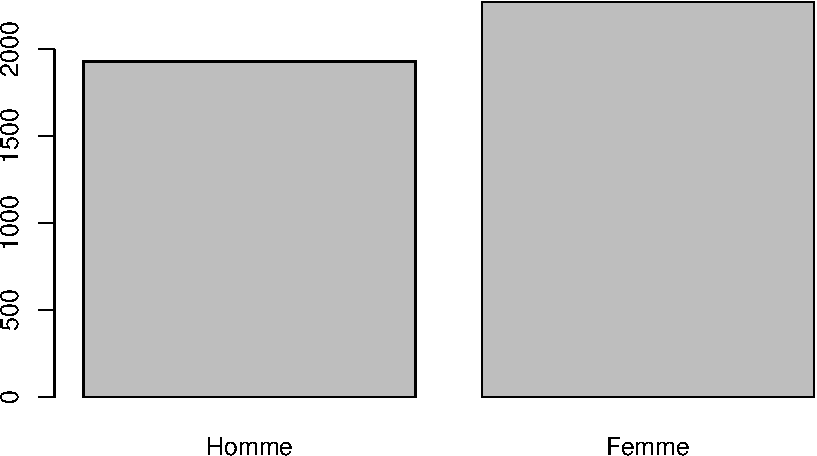
\includegraphics{_main_files/figure-latex/unnamed-chunk-35-1.pdf}

\begin{Shaded}
\begin{Highlighting}[]
\CommentTok{\# le plus approprié pour le type de variable.}
\end{Highlighting}
\end{Shaded}

Nous pourrions aussi enregistrer cette figure quelque part sur notre ordinateur.

\begin{Shaded}
\begin{Highlighting}[]
\FunctionTok{jpeg}\NormalTok{(}\StringTok{\textquotesingle{}hist.jpg\textquotesingle{}}\NormalTok{) }\CommentTok{\# créé un fichier jpeg (ce pourrait être un autre type)}
\CommentTok{\# qui sera prêt à recevoir du contenu que nous ferons à la prochaine ligne.}

\FunctionTok{plot}\NormalTok{(ces15}\SpecialCharTok{$}\NormalTok{sexe) }\CommentTok{\# fait l\textquotesingle{}histogramme}

\FunctionTok{dev.off}\NormalTok{() }\CommentTok{\# referme la création de figure temprairement ouverte par }
\end{Highlighting}
\end{Shaded}

\begin{verbatim}
## pdf 
##   2
\end{verbatim}

\begin{Shaded}
\begin{Highlighting}[]
\CommentTok{\# la première commande.}
\end{Highlighting}
\end{Shaded}

Nous aurons alors le fichier «hist.jpg» qui sera sauvegardé là où a été établi notre «working directory». Si nous avions voulu enregistrer ce fichier ailleurs, il aurait simplement fallu écrire le chemin complet vers cet endroit. Par exemple, pour sauvegarder la figure sur notre bureau, on aurait fait ceci:

\begin{Shaded}
\begin{Highlighting}[]
\FunctionTok{jpeg}\NormalTok{(}\StringTok{"/Users/alexandreblanchet/Desktop/hist.jpg"}\NormalTok{) }\CommentTok{\# sauvegarde sur le bureau}
\CommentTok{\# au lieu du working directory}
\FunctionTok{plot}\NormalTok{(ces15}\SpecialCharTok{$}\NormalTok{sexe,}
     \AttributeTok{main=}\StringTok{"La figure de l\textquotesingle{}année!"}\NormalTok{, }\CommentTok{\# spécifier un titre à la figure}
     \AttributeTok{ylab=}\StringTok{"Fréquence"}\NormalTok{)  }\CommentTok{\# Spécifier un label pour l\textquotesingle{}axe Y}

\CommentTok{\# J\textquotesingle{}en profite pour mettre un titre et un label à l\textquotesingle{}axe Y.}
\CommentTok{\# Notez l\textquotesingle{}ajouts de virgules, qui annoncent qu\textquotesingle{}il y aura autre}
\CommentTok{\# chose. Notez aussi que la parenthèse ouverte à plot( se referme après }
\CommentTok{\# avoir spécifié les options ajoutées.}
\FunctionTok{dev.off}\NormalTok{() }
\end{Highlighting}
\end{Shaded}

\begin{verbatim}
## pdf 
##   2
\end{verbatim}

Évidemment, le lien est valable pour le bureau de mon ordinateur à moi et il faudrait modifier le lien pour qu'il correspondent au vôtre.

\hypertarget{tableau-croisuxe9}{%
\section{Tableau croisé}\label{tableau-croisuxe9}}

Nous voulons souvent faire des tableaux croisés poru voir comment deux variables sont liées. Imaginons que nous voulions voir dans quelle langue les hommes et les femmes ont répondu au sondage.

\begin{Shaded}
\begin{Highlighting}[]
\FunctionTok{table}\NormalTok{(ces15}\SpecialCharTok{$}\NormalTok{CPS15\_INTLANG)}
\end{Highlighting}
\end{Shaded}

\begin{verbatim}
## 
##    1    5 
## 3472  730
\end{verbatim}

Nous avons 3472 personnes qui sont codées 1 (anglais) et 730 personnes qui sont codées 5 (français). Nous pouvons modifier ces codes par les labels.

\begin{Shaded}
\begin{Highlighting}[]
\NormalTok{ces15}\SpecialCharTok{$}\NormalTok{langue\_int }\OtherTok{\textless{}{-}} \FunctionTok{factor}\NormalTok{(ces15}\SpecialCharTok{$}\NormalTok{CPS15\_INTLANG, }
                          \AttributeTok{labels =} \FunctionTok{c}\NormalTok{(}\StringTok{"Anglais"}\NormalTok{, }\StringTok{"Français"}\NormalTok{))}
\CommentTok{\# Notez qu\textquotesingle{}encore une fois j\textquotesingle{}ai créé une nouvelle variable "langue\_int" }
\CommentTok{\# plutôt que de modifier la variable originale CPS15\_INTLANG. }
\FunctionTok{table}\NormalTok{(ces15}\SpecialCharTok{$}\NormalTok{langue\_int)}
\end{Highlighting}
\end{Shaded}

\begin{verbatim}
## 
##  Anglais Français 
##     3472      730
\end{verbatim}

Puis nous pouvons faire le tableau croisé avec la variable de sexe:

\begin{Shaded}
\begin{Highlighting}[]
\FunctionTok{table}\NormalTok{(ces15}\SpecialCharTok{$}\NormalTok{langue\_int, ces15}\SpecialCharTok{$}\NormalTok{sexe)}
\end{Highlighting}
\end{Shaded}

\begin{verbatim}
##           
##            Homme Femme
##   Anglais   1592  1880
##   Français   338   392
\end{verbatim}

Nous obtenons ici les fréquences pour chaque caractéristiques croisées. Nous pourrions cependant vouloir les pourcentages.

\begin{Shaded}
\begin{Highlighting}[]
\NormalTok{tableau\_sexelangue }\OtherTok{\textless{}{-}} \FunctionTok{table}\NormalTok{(ces15}\SpecialCharTok{$}\NormalTok{langue\_int, ces15}\SpecialCharTok{$}\NormalTok{sexe) }\CommentTok{\# Nous plaçons }
\CommentTok{\# d\textquotesingle{}abord le tableau croisé prédédent dans l\textquotesingle{}objet tableau\_sexelangue, }
\CommentTok{\# puis nous pourrons utiliser cet objet pour demander à R de compiler}
\CommentTok{\# les pourcentage via la commande prop.table()}

\FunctionTok{prop.table}\NormalTok{(tableau\_sexelangue, }\DecValTok{1}\NormalTok{) }\CommentTok{\# Proportions en rangées}
\end{Highlighting}
\end{Shaded}

\begin{verbatim}
##           
##                Homme     Femme
##   Anglais  0.4585253 0.5414747
##   Français 0.4630137 0.5369863
\end{verbatim}

\begin{Shaded}
\begin{Highlighting}[]
\FunctionTok{prop.table}\NormalTok{(tableau\_sexelangue, }\DecValTok{2}\NormalTok{) }\CommentTok{\# Proportions en colones}
\end{Highlighting}
\end{Shaded}

\begin{verbatim}
##           
##                Homme     Femme
##   Anglais  0.8248705 0.8274648
##   Français 0.1751295 0.1725352
\end{verbatim}

\begin{Shaded}
\begin{Highlighting}[]
\CommentTok{\# Si nous voulions avoir les proportions sur 100 (pourcentages)}
\CommentTok{\# plutôt que sur 1, nous pourrions simplement ajouter "*100".}
\FunctionTok{prop.table}\NormalTok{(tableau\_sexelangue, }\DecValTok{1}\NormalTok{)}\SpecialCharTok{*}\DecValTok{100} \CommentTok{\# Pourcentages en rangées}
\end{Highlighting}
\end{Shaded}

\begin{verbatim}
##           
##               Homme    Femme
##   Anglais  45.85253 54.14747
##   Français 46.30137 53.69863
\end{verbatim}

\begin{Shaded}
\begin{Highlighting}[]
\FunctionTok{prop.table}\NormalTok{(tableau\_sexelangue, }\DecValTok{2}\NormalTok{)}\SpecialCharTok{*}\DecValTok{100} \CommentTok{\# Pourcentages en colones}
\end{Highlighting}
\end{Shaded}

\begin{verbatim}
##           
##               Homme    Femme
##   Anglais  82.48705 82.74648
##   Français 17.51295 17.25352
\end{verbatim}

Nous pourrions continuer à voir séparément différentes fonctions de R, mais cela deviendrait vite interminable. Vous devriez maintenant avoir les bases pour saisir la logique de la syntaxe de R et pour avoir une idée générale de ce qu'est une syntaxe. C'est ce qui est important. Il est impossible de couvrir le fonctionnement de R sans aussi apprendre à faire des statistiques. Si vous décidez d'apprendre R, vous devrez de toute manière apprendre par essai-erreur et cela viendra avec la pratique. Google sera votre plus grand ami!

Tournons-nous maintenant sur l'objectif principal de toute analyse statistique : décrire.

\hypertarget{duxe9crire}{%
\chapter{Décrire}\label{duxe9crire}}

Si nous voulions décrire la taille de Serge, nous pourrions par exemple dire qu'il mesure 180cm. Si nous voulions décrire la taille de Serge et Janette, nous pourrions dire que Serge mesure 180cm et que Janette mesure 170cm. Si nous voulions décrire la taille de Serge, Janette et Albert, nous pourrions dire que Serge mesure 180cm, Janette 170cm et Albert 160cm. Nous pourrions continuer d'ajouter des personnes et décrire leur taille, mais à mesure que le nombre de personnes augmentera, il deviendra de plus en plus difficile de décrire la taille des personnes qui nous intéressent en se référant à la taille individuelle de chaque personne. Même l'individu le plus intelligent du monde ne parviendra pas à manipuler simultanément dans sa tête les tailles individuelles de 30 personnes (voir même 10). Pour cette raison, décrire des données implique aussi nécessairement les de \emph{synthétiser}.

Évidemment, on peut décrire un seul élément, mais aussi vouloir décrire la relation entre deux ou plusieurs éléments. En sciences sociales, nous nous intéressons à des choses qui varient. Les choses qui ne varient pas ne nous intéressent généralement pas, justement parce qu'elles ne varient pas. Par exemple, le fait que chaque personne lisant ce texte soit née sur terre (il n'y a pas d'humains né ailleurs que sur terre) est aussi rassurant qu'innintéressant. En statistiques, nous dirons donc que nous nous intéressons aux «variables» qui sont des «choses qui varient» (tadam!), par opposition aux choses qui ne varient pas, qui sont des constantes. Ainsi, lorsque nous cherchons à décrire un phénomène, nous voulons, en termes statistiques, décrire une variable ou des relations entre variables. Concentrons-nous pour l'instant sur la description d'une seule variable.

\hypertarget{une-uxe9quation-pour-duxe9crire-une-variable}{%
\section{Une équation pour décrire une variable}\label{une-uxe9quation-pour-duxe9crire-une-variable}}

Je voudrais maintenant que vous lisiez l'équation ci-dessous sans lire ce qui vient sous la section «La réponse». Je vais ici décrire ce que veulent dire les symboles et je voudrais que vous réfléchissiez à ce que peut bien vouloir dire cette équation. L'objectif est tout simplement de commencer à vous habituer à réfléchir en termes mathématiques, et surtout de vous faire voir que les formules n'ont rien de magique si l'on prend simplement le temps de s'y arrêter un peu.

\hypertarget{quest-ce-que-cette-uxe9quation}{%
\subsection{Qu'est-ce que cette équation?}\label{quest-ce-que-cette-uxe9quation}}

\[? = \frac { 1 }{ n } \sum_{ i=1 }^{ n }{ x_i }\]
Le signe \(\sum\) peut se lire comme «la somme de tout ce qui vient à droite». \(x_i\) représente la valeur d'un individu \(i\) sur la variable \(x\). Donc, \(\sum x_i\) implique que nous fassions la somme de toues les \(x\) individuels. Imaginez \(x\) comme étant le nom d'une colonne dans un fichier excel et chaque \(x_i\) représente une cellule particulière de cette colonne. Par exemple, \(x_1\) réfère à la valeur de \(x\) à la ligne 1, \(x_2\) la valeur de \(x\) à la ligne 2, etc. \(i=1\) sous le signe de \(\sum\) signifie que la somme qui nous intéresse commence à la ligne 1. Le \(n\) au-dessus du signe de \(\sum\) signifie que nous arrêtons l'addition à \(n\). C'est donc dire qu'ici, nous additionnons toutes les valeurs individuelles de \(x_1\) à \(x_n\), autrement dit les valeurs de \(x\) pour toutes les lignes.

Donc, \(\sum_{ i=1 }^{ n }{ x_i }\) signifie que nous additionnons toutes les valeurs individuelles de \(x\). Nous voyons ensuite que \(\sum_{ i=1 }^{ n }{ x_i }\) est multiplié par \(\frac { 1 }{ n }\).

Réfléchissez un instant à ce que veut dire cette équation avant de passer à la section «La réponse». Qu'est-ce que peut bien nous donner le fait d'additionner toutes les lignes d'une colonne (\(\sum_{ i=1 }^{ n }{ x_i }\)) et de multiplier cette somme par \(\frac { 1 }{ n }\)?

\hypertarget{la-ruxe9ponse}{%
\subsection{La réponse}\label{la-ruxe9ponse}}

L'équation ci-dessus est tout simplement celle qui nous permet de calculer la moyenne d'une variable. Il s'agit de l'équation «officielle». Si vous n'avez pas trouvé la réponse, la raison est probablement que ce n'est pas de cette manière que la plupart d'entre-nous calculons une moyenne. Habituellement, nous faisons la somme des valeurs d'une variable (donc \(\sum_{ i=1 }^{ n }{ x_i }\)) et nous divisons cette somme par le nombre d'unités de cette variable (ou \(n\)). Autrement dit, ce que vous avez probablement tendance à faire est l'équation suivante :

\[\bar{x} = \frac { \sum_{ i=1 }^{ n }{ x_i } }{ n }\]
Cette équation est équivalente à la première, mais réfléchissons quelques instants pour bien comprendre pourquoi elles donnent forcément le même résultat.

Les deux équations sont formées de la même somme \(\sum_{ i=1 }^{ n }{ x_i }\) qui est soit divisée par \(n\), soit multipliée par \(\frac { 1 }{ n }\). Si par exemple nous nous intéressions à la taille moyenne d'un groupe de 50 individus, \(\sum_{ i=1 }^{ 50 }{ x_i }\) veut donc dire que nous additionnons la taille de chaque individu (\(x_i\)) pour obtenir la taille totale du groupe en entier. Lorsque vous calculez une moyenne, vous avez probablement tendance a diviser la somme totale du groupe par \(n\), ici le nombre d'individus dans notre groupe, soit 50. En divisant la somme totale du groupe par le nombre d'individus qui le compose, on se trouve donc à «répartir» la taille totale du groupe parmi les 50 individus. C'est tout à fait correct et logique. Cependant, remarquez comment, plutôt que de «répartir» la somme totale sur \(n\), la première équation donne plutôt un «poids» à chaque individu en divisant 1 par \(n\).

Imaginons que la taille totale de nos 50 individus donne 9000cm (\(\sum_{ i=1 }^{ n }{ x_i }\)=9000). La formule que vous utilisez habituellement serait donc \(\bar{x}= \frac{9000}{50} = 180\). Si nous procédons plutôt en suivant la première formule, nous remarquons d'abord que \(\frac{1}{50}\) = 0.02. Dans un groupe de 50, un individu représente donc \(\frac{1}{50}\), ou 0.02 du total des individus. La première formule revient donc à faire \(\bar{x}= 0.02 \times 9000 = 180\).

Avec la première formule, nous voulons donc obtenir une certaine proportion (ici 0.02, ou \(\frac{1}{50}\)) du total des \(x_i\), alors qu'avec la formule «habituelle», on «réparti» ce total sur le nombre d'éléments dont il est composé. Plutôt que de «répartir» la taille totale sur le nombre d'individus, la première formule «pondère» le poids de chaque individu en remenant le «poids» d'un seul individu sur le total du groupe sur une unité de 1 (\(\frac{1}{n}\)). La logique est légèrement différente, mais elle revient au même.

\hypertarget{une-uxe9quation-guxe9nuxe9rale-duxe9crivant-la-variable}{%
\subsection{Une équation générale décrivant la variable?}\label{une-uxe9quation-guxe9nuxe9rale-duxe9crivant-la-variable}}

L'objectif de la section précédente était tout simplement de vous faire voir la «mécanique» d'une équation avec quelque chose que la plupart d'entre-vous utilisez régulièrement. L'exemple de la moyenne nous permet aussi de voir comment deux logiques différentes, mais équivalentes, peuvent aussi être écrites de manière différentes mathématiquement. En utilisant le concept de moyenne que la plupart d'entre-vous connaissez bien, je tente de diminuer votre angoisse \citep{tobias1993} matématique face aux équations!

Ceci étant, l'un des avantages des équations est qu'elles nous permettent aussi de proposer une description claire et succincte d'une variable. Imaginons que nous voulions décrire la variable \(x\) en une seule équation et de manière la \emph{plus complète possible}. En conservant notre exemple du groupe de 50 personnes ayant une taille moyenne de 180cm, nous pourrions dire que la moyenne de \(x\) = 180cm et cette information est très certainement utile. Cependant, la moyenne du groupe demeure tout de même une information générale qui n'est pas forcément vraie pour chaque personne, elle nous informe sur le groupe entier, pas sur chaque individu spécifique. Nous pourrions cependant utiliser la moyenne afin de décrire la variable à l'aide d'une équation qui sera «vraie» pour chaque individu. C'est ce que fait l'équation suivante :
\[x_i= \frac { 1 }{ n } \sum_{ i=1 }^{ n }{ x_i } + e_i\]
Ici, \(x_i\) équivaut encore à la valeur de \(x\) pour l'individu \(i\). Remarquons que la formule est pratiquement identique à la formule de la moyenne, mais nous y avons ajouté \(+ e_i\), où \(e_i\) signifie \emph{l'écart} de chaque individu \(i\) par rapport à la moyenne (\(\frac { 1 }{ n } \sum_{ i=1 }^{ n }{ x_i } = 180\)).

Donc, si par exemple l'individu 2 mesure 190cm (\(x_2 = 190\)), la valeur de \(e_2\) sera de 10. Ainsi, \(x_2 = 180 + 10 = 190\) et nous voyons que l'équation proposée décrit adéquatement l'individu 2. Si si l'individu 3 mesure 170cm (\(x_3 = 170\)), la valeur de \(e_3\) sera de -10. \(e_i\) équivaut donc à la distance d'un individu par rapport à la moyenne du groupe.

Ces écarts individuels à la moyenne peuvent être mis au carré (pour éliminer les signes négatifs) et additionnés ensemble. Cela nous donne ce que nous appelons la \emph{somme du carré des écarts}, c'est-à-dire le grand total de tous les \(e_i\) mis à la 2 (\(e_i^2\)). L'une des propriété de la moyenne est qu'elle est le nombre qui \emph{minimise} cette somme. Aucun autre nombre que la moyenne d'une distribution ne peut donner une \emph{somme du carré des écarts} plus petite. Une moyenne n'est pas forcément le meilleur nombre à utiliser pour synthétiser une variable, mais la moyenne est systématiquement le chiffre qui est le plus proche de toutes les valeurs individuelles d'une variable donnée. Nous verrons plus tard que la régression présente une caractéristique similaire et il est donc utile que vous compreniez pourquoi cette caractéristique est intéressante à partir du concept de moyenne que vous maîtrisez déjà.

Le concept d'écart individuel à la moyenne est aussi très utile parce qu'il nous permet d'écrire une règle générale qui décrira précisément toutes nos données et ce en tenant compte de la variation individuelle autour de notre moyenne. Pour une équation générale, nous pourrions simplifier encore plus et écrire :
\[x_i= \bar{x} + e_i\]
Où \(\bar{x}\) (prononcé «x-barre») a simplement remplacé l'équation plus détaillée de la moyenne. La taille précise de l'individu 2 décrit plus haut peut être écrite :
\[x_2= \bar{x} + e_2\]
\[x_2 = 180 + 10 = 190\]

Vous voyez donc que l'on peut décrire de manière succincte une variable en établissant une caractéristique de cette variable qui s'applique à tout le groupe (ici la moyenne du groupe) et en y ajoutant la \emph{déviation} (ou l'écart) de chaque individu par rapport à cette caractéristique commune. Ce qui varie d'un individu à l'autre (les valeurs de \(x\) et \(e\)) sont indicés par \(i\) (\(x_i\) et \(e_i\)), alors que ce qui est valable pour tout le groupe (la moyenne) n'a pas d'indice (\(\bar{x}\)). Les indices nous permettent de spécifier plus clairement ce à quoi nous référons. Ceci étant, il arrive fréquemment qu'ils soient omis lorsqu'il n'y a aucun doute sur l'interprétation d'une équation.

Il est fort probable que vous ne décriviez jamais la moyenne d'un groupe d'individus avec l'équation que nous venons de voir, mais l'objectif était simplement de vous faire voir comment on peut formuler une description générale valable pour tous les individus d'un groupe à partir d'une caractéristique commune au groupe. L'idée n'est donc pas ici que vous appliquiez cette formule, mais que vous compreniez le concept derrière l'idée de «déviation» individuelle par rapport à la caractéristique commune. Cette compréhension intuitive vous sera très utile lorsque nous arriverons à la régression.

Il y a bien sûr de nombreuses autres manières de décrire une variable.

\begin{itemize}
\tightlist
\item
  Les mesures de tendances centrales : mode, médiane, moyenne
\item
  Les mesures de variation : étendue, variance, écart-type
\item
  Les mesure d'asymétrie : coefficient d'asymétrie
\end{itemize}

\hypertarget{les-types-de-variables-et-uxe9viter-de-faire-nimporte-quoi}{%
\section{Les types de variables et éviter de faire n'importe quoi}\label{les-types-de-variables-et-uxe9viter-de-faire-nimporte-quoi}}

La manière la plus adéquate de décrire une variable est aussi liée au \emph{type de variable}. Les variables peuvent être :

\begin{itemize}
\tightlist
\item
  Nominales

  \begin{itemize}
  \tightlist
  \item
    Une variable qui décrit des états différents qui ne sont pas ordonnancés hiérarchiquement.
  \item
    Les catégories doivent être exhaustives et mutuellement exclusives.
  \item
    Exemples : la couleur des yeux ou des cheveux. Le choix de vote (PLQ, PQ, CAQ, QS).
  \end{itemize}
\item
  Ordinales

  \begin{itemize}
  \tightlist
  \item
    Une variable qui varie en fonction de différents états qui \emph{peuvent} être ordonnancés hiérarchiquement, mais dont la distance entre ces états ne peut être réellement établie.
  \item
    Exemples : très satisfait, satisfait, insatisfait, très insatisfait. Un peu, beaucoup, pationnément, à la folie.
  \end{itemize}
\item
  Continues (parfois appelées «d'intervalles/ratio»)

  \begin{itemize}
  \tightlist
  \item
    Une variable qui peut être mesurée par une unité standard.
  \item
    Exemples: le poids, la taille, la distance, le temps.
  \end{itemize}
\item
  Dichotomiques (parfois appelées «dummy»)

  \begin{itemize}
  \tightlist
  \item
    Comme les variables nominales, mais avec seulement deux catégories.
  \item
    Exemples : homme/femme, riche/pauvre, avoir un diplôme uiversitaire/ne pas en avoir.
  \end{itemize}
\end{itemize}

Contrairement aux variables nominales et ordinales, les variables dichotomiques ont cetains avantages qui viennent du fait qu'elles n'ont que deux catégories. Elles peuvent notamment être taitées numériquement (0 et 1) même si les chiffres 0 et 1 réfèrent à des catégories distinctes qui ne sont pas ordonancées hiérarchiquement. Par exemple, il ne fait aucun sens de faire la moyenne d'une variable nominale ou ordinale : calculer la moyenne de la couleur des yeux des gens dans une classe n'a pas de sens. Par contre, même s'il ne fait pas de sens de calculer la «moyenne du sexe» des gens dans une classe, cette moyenne nous donnera quand même un chiffre interprétable : la proportion d'hommes et de femmes. Par exemple, si nous avons 4 hommes (codés 0) et 6 femmes (codées 1), la moyenne nous donnera \(\frac{6}{10}\) = 0.6, donc la proportion de la catégorie qui est codée 1, ici les femmes. Inversement, nous saurons aussi forcément qu'il y a 40\% d'hommes.

Ceci étant, lorsque l'on fait des analyses statistiques, il est important de faire attention au type de variables que nous utilisons si l'on veut les décrire adéquatement. C'est également le cas lorsque nous voulons décrire une relation entre deux variables. Peu importe le type de variable, les logiciels et les procédures statistiques traitent des colones de nombres. \emph{Un logiciel n'a aucune idée de ce que ce que ces nombres veulent dire, ni s'il fait du sens de faire la procédure que vous lui demandez d'effectuer}.

Si vous avez un groupe d'individus et que vous vous intéressez à la couleur de leurs yeux qui peuvent être bleus (codé 1), bruns (codé 2), pairs (codé 3), ou verts (codé 4); le logiciel vous donnera un résultat si vous lui demandez la moyenne de la couleurs de leurs yeux. Le nombre n'aura aucun sens, mais le logiciel ne le saura pas. Il aura simplement calculé la moyenne des nombre codés de 1 à 4 dans la colone «couleur des yeux» sans savoir qu'ils réfèrent en fait à des couleurs. C'est à vous de le savoir. Nous verrons en chemin que les logiciels peuvent traiter des variables de plusieurs format -- par exemple des variables numériques ou des variables de facteur (bleu, brun, pair, vert au lieu des nombres), et ces différents types de variables peuvent être traitées différemment suivant les logiciels. Au final cependant, tout est en quelque part transformé en un chiffre. C'est à vous de vous assurer que le tout fait du sens et \emph{aucune procédure statistique ne peut se substituer à votre jugement}.

\hypertarget{duxe9crire-une-relation-entre-des-variables}{%
\section{Décrire une relation entre des variables}\label{duxe9crire-une-relation-entre-des-variables}}

Si bien sûr nous pouvons souvent nous intéresser à la description d'une seule variable (par exemple : pour quel parti les gens ont le plus l'intention de voter lors des prochaines élections?), on s'intéresse aussi souvent à la \emph{relation} entre des variables. La raison en est tout simplement que nous cherchons des \emph{explications} à un phénomène (une variable) qui nous intéresse et nous désirons donc voir si le phénomène diffère (si la variable varie) en fonction d'un autre phénomène. Pour cette raison, nous nous intéressons souvent aux corrélations entre des variables.

Une mesure souvent utilisée pour évaluer la relation entre deux variables est le coefficient de corrélation. Ce coefficient varie en -1 et 1. Un coefficient de 1 indique une relation positive parfaite, un coefficient de -1 une relation négative parfaite et un coefficient de 0 indique une absence «parfaite» de relation entre les variables. Par exemple, imaginons que nous avons les variables suivantes pouitA, pouitB, pouitC et pouitD :

\begin{Shaded}
\begin{Highlighting}[]
\NormalTok{pouitA }\OtherTok{\textless{}{-}} \FunctionTok{c}\NormalTok{(}\DecValTok{1}\NormalTok{, }\DecValTok{2}\NormalTok{, }\DecValTok{3}\NormalTok{, }\DecValTok{4}\NormalTok{, }\DecValTok{5}\NormalTok{)}
\NormalTok{pouitB }\OtherTok{\textless{}{-}} \FunctionTok{c}\NormalTok{(}\DecValTok{6}\NormalTok{, }\DecValTok{7}\NormalTok{, }\DecValTok{8}\NormalTok{, }\DecValTok{9}\NormalTok{, }\DecValTok{10}\NormalTok{) }\CommentTok{\# Similaire à pouitA, mais de 6 à 10}
\NormalTok{pouitC }\OtherTok{\textless{}{-}} \FunctionTok{c}\NormalTok{(}\DecValTok{5}\NormalTok{, }\DecValTok{4}\NormalTok{, }\DecValTok{3}\NormalTok{, }\DecValTok{2}\NormalTok{, }\DecValTok{1}\NormalTok{) }\CommentTok{\# Inverse de pouitA}
\NormalTok{pouitD }\OtherTok{\textless{}{-}} \FunctionTok{c}\NormalTok{(}\DecValTok{2}\NormalTok{, }\DecValTok{1}\NormalTok{, }\DecValTok{2}\NormalTok{, }\DecValTok{5}\NormalTok{, }\DecValTok{4}\NormalTok{) }\CommentTok{\# Quelques variations par rapport à pouitA}
\end{Highlighting}
\end{Shaded}

PouiA et PouitB auront une corrélation de 1, alors que PouitC aura une corrélation de -1 avec PouitA et PouitB. À vue d'oeil, PouitD devrait avoir une corrélation d'autour de 0.75 avec pouitA et pouitB, et d'environ -0.75 avec pouitC.

\begin{Shaded}
\begin{Highlighting}[]
\CommentTok{\# Corrélation entre PouitA et PouitB}
\FunctionTok{cor}\NormalTok{(pouitA, pouitB) }\CommentTok{\# cor() pour "correlation"}
\end{Highlighting}
\end{Shaded}

\begin{verbatim}
## [1] 1
\end{verbatim}

\begin{Shaded}
\begin{Highlighting}[]
\CommentTok{\# Corrélation entre PouitA et PouitC}
\FunctionTok{cor}\NormalTok{(pouitA, pouitC) }\CommentTok{\# Quand puitA augmente, pouitC diminue}
\end{Highlighting}
\end{Shaded}

\begin{verbatim}
## [1] -1
\end{verbatim}

\begin{Shaded}
\begin{Highlighting}[]
\CommentTok{\# Corrélation entre PouitB et PouitC}
\FunctionTok{cor}\NormalTok{(pouitB, pouitC) }\CommentTok{\# Quand puitB augmente, pouitC diminue}
\end{Highlighting}
\end{Shaded}

\begin{verbatim}
## [1] -1
\end{verbatim}

\begin{Shaded}
\begin{Highlighting}[]
\CommentTok{\# Corrélation entre PouitA et PouitD}
\FunctionTok{cor}\NormalTok{(pouitA, pouitD) }\CommentTok{\# Quand puitA augmente, pouitD augmente}
\end{Highlighting}
\end{Shaded}

\begin{verbatim}
## [1] 0.7698004
\end{verbatim}

\begin{Shaded}
\begin{Highlighting}[]
\CommentTok{\# Corrélation entre PouitB et PouitD}
\FunctionTok{cor}\NormalTok{(pouitB, pouitD) }\CommentTok{\# Quand puitB augmente, pouitD augmente}
\end{Highlighting}
\end{Shaded}

\begin{verbatim}
## [1] 0.7698004
\end{verbatim}

\begin{Shaded}
\begin{Highlighting}[]
\CommentTok{\# Corrélation entre PouitC et PouitD}
\FunctionTok{cor}\NormalTok{(pouitC, pouitD) }\CommentTok{\# Quand puitC augmente, pouitD diminue}
\end{Highlighting}
\end{Shaded}

\begin{verbatim}
## [1] -0.7698004
\end{verbatim}

\begin{Shaded}
\begin{Highlighting}[]
\CommentTok{\# Débarassons{-}nous de ces pouits...}
\FunctionTok{rm}\NormalTok{(pouitA, pouitB, pouitC, pouitD) }\CommentTok{\# rm() pour "remove" comme vu plus haut.}
\end{Highlighting}
\end{Shaded}

En règle générale, un coefficient de 0.5 (ou de -0.5) ou plus en sciences sociales est généralement considéré comme relativement fort. Plus le chiffre en termes absolu (c'est-à-dire sans tenir compte du signe négatif ou positif) est élevé, plus la relation est forte. Cependant, nous ne nous étendrons pas ici sur ce coefficient ni sur son calcul puisqu'il est relativement simple et que je souhaite que nous nous concentrions sur la régression, qui est abondement utilisée en méthodes quantitatives. Aussi, faites attention de \emph{ne pas confondre les coefficients de corrélation avec les coefficients de régression}. Un coefficient de régression de 0.25 (ou même de 0.02) peut être très fort dépendemment de l'échelle de mesure des variables concernées.

Ceci étant, une chose doit être précisée dès le début : \emph{la corrélation n'équivaut pas à la causalité!} La question de la causalité est très complexe et controversée. Gardons-nous donc d'en discuter et contentons-nous de dire que nous cherchons à \emph{comprendre} un phénomène qui nous intéresse\footnote{Pour un livre intéressant sur cette question et nuancé sur le positivisme général, voir \citet{favre2005}.}. Par \emph{comprendre}, nous voulons donc dire que nous voulons \emph{expliquer} ce qui fait en sorte que le phénomène survient ou non, ou mieux décrire comment au juste il survient. Nous avons une certaine thèse sur les facteurs qui font en sorte que le phénomène advient ou n'advient pas, ou qu'il advient d'une manière plutôt que d'une autre. Trois règles logiques doivent minimalement être respectées :

\begin{enumerate}
\def\labelenumi{\arabic{enumi}.}
\tightlist
\item
  La chose qui explique le phénomène doit être antérieure (temporellement, logiquement, ou théoriquement) à celui-ci.

  \begin{itemize}
  \tightlist
  \item
    Temporellement : ce qui arrive aujourd'hui ne peut expliquer ce qui est arrivé hier. C'est bêtement logique.
  \item
    Théoriquement : Même si une explication potentielle est temporellement antérieure à un phénomène, il faut avoir un argument raisonnable pour affirmer qu'ils sont liés. Cet argument (ou idéalement \emph{ces} arguments) n'a pas grand-choses à voir avec les statistiques. Il s'agit ici de réflexion théorique et empirique.
  \end{itemize}
\item
  Pour qu'une chose en explique une autre, elle doit lui être liée d'une manière ou d'une autre. Ceci implique donc forcément la présence d'une association entre le facteur explicatif et le phénomène que l'on veut expliquer.

  \begin{itemize}
  \tightlist
  \item
    En méthode quantitatives, cela implique que les deux éléments doivent être associés statistiquement. C'est-à-dire que les valeurs des deux éléments doivent être corrélées.
  \item
    Une corrélation peut être \emph{positive} : quand les valeurs d'une variable sont élevées, celles d'une autre variable ont tendance à être plus élevées.
  \item
    Une corrélation peut être \emph{négative} : quand les valeurs d'une variable sont élevées, celles d'une autre variable ont tendance à être plus faibles, ou inversement.
  \end{itemize}
\item
  Le lien entre le facteur explicatif et le phénomène d'intérêt ne doit pas être fallacieux, c'est-à-dire qu'il ne doit pas être généré par un autre facteur qui explique les deux éléments initiaux.

  \begin{itemize}
  \tightlist
  \item
    Par exemple, si l'on remarque que les dégâts lors d'un incendie sont plus importants lorsqu'il y a plus de pompiers pour le combattre, il serait évidemment fallacieux d'en conclure que les pompiers causent les dégâts. C'est \emph{l'intensité} de l'incendie qui rend nécessaire la présence d'un plus grand nombre de pompiers pour le combattre \emph{et} c'est aussi cette intensité qui explique que les dégâts sont plus importants. Le fait qu'il y ait plus de dégâts quand il y a plus de pompiers (une simple association statistique) n'implique absoluement pas que les pompiers produisent les dégâts.
  \end{itemize}
\end{enumerate}

\hypertarget{la-ruxe9gression-linuxe9aire-simple-avec-une-variable-dichotomique}{%
\section{La régression linéaire simple avec une variable dichotomique}\label{la-ruxe9gression-linuxe9aire-simple-avec-une-variable-dichotomique}}

Mon objectif est ici que vous développiez une compréhension intuitive de ce qu'est la régression linéaire et de ce que les résultats veulent dire au juste. Nous n'allons pas nous amuser à calculer à la main des régressions, mais nous allons en faire avec des données que nous créerons nous-mêmes. Pour cette section, oubliez les étoiles et concentrez-vous uniquement les coefficients. Les coefficients permettent de \emph{décrire} les données, les étoiles ont trait à l'inférence. Or avant d'inférer quoique ce soit, encore faut-il le décrire.

\hypertarget{cruxe9ation-des-donnuxe9es}{%
\subsection{Création des données}\label{cruxe9ation-des-donnuxe9es}}

Nous allons ici créer des données que nous inventerons nous-mêmes pour fins d'illustration. Nous nous intéresserons aux notes qu'un groupe de 100 élèves ont reçu à leur dernier examen du cours d'introduction à la pétanque full contact (PFC 1000). Nous nous pencherons sur l'impact du sexe des élèves et du nombre d'heures d'étude sur la note qu'ils ont reçu.

La syntaxe ci-bas crée les données et quelques explications sont fournies en annotation. Vous n'avez cependant pas à comprendre cette syntaxe pour comprendre ce qui suivra.

\begin{Shaded}
\begin{Highlighting}[]
\CommentTok{\# Pour réplication }
\FunctionTok{set.seed}\NormalTok{(}\DecValTok{987654321}\NormalTok{) }\CommentTok{\# R génère des chiffres aléatoirement et pour}
\CommentTok{\# qu\textquotesingle{}il le fasse de manière constante d\textquotesingle{}une fois à l\textquotesingle{}autre, on}
\CommentTok{\# peut lui dire de le faire d\textquotesingle{}une manière exacte. Si vous ne le faites pas,}
\CommentTok{\# vous obtiendrez probablement des résultats différents de ceux du document}
\CommentTok{\# tout simplement parce que R génèrera aléatoirement des données un peu }
\CommentTok{\# différentes.}

\NormalTok{fille }\OtherTok{\textless{}{-}} \FunctionTok{rbinom}\NormalTok{(}\DecValTok{100}\NormalTok{, }\DecValTok{1}\NormalTok{, }\DecValTok{1}\SpecialCharTok{/}\DecValTok{2}\NormalTok{)}\CommentTok{\# créer 100 individus qui ont une chance de }
\CommentTok{\# 1/2  d\textquotesingle{}être codé 1 dans l\textquotesingle{}objet "fille", les autres seront codés 0. }

\NormalTok{heures.etude }\OtherTok{\textless{}{-}} \FunctionTok{rnorm}\NormalTok{(}\DecValTok{100}\NormalTok{, }\AttributeTok{mean=}\FloatTok{4.5} \SpecialCharTok{+} \FloatTok{1.5}\SpecialCharTok{*}\NormalTok{fille, }\AttributeTok{sd=}\FloatTok{1.5}\NormalTok{ ) }\CommentTok{\# Crée la variable}
\CommentTok{\# heures études avec une moyenne de 4.5, les filles qui étudient en moyenne }
\CommentTok{\# 1.5 heures de plus que la garçons, le tout avec une erreur standard de }
\CommentTok{\# 1.5 pour mettre une peu de variation dans tout cela.}

\NormalTok{notes }\OtherTok{\textless{}{-}} \FunctionTok{rnorm}\NormalTok{(}\DecValTok{100}\NormalTok{, }\AttributeTok{mean=}\DecValTok{35} \SpecialCharTok{+} \DecValTok{4}\SpecialCharTok{*}\NormalTok{fille }\SpecialCharTok{+} \DecValTok{5}\SpecialCharTok{*}\NormalTok{heures.etude, }\AttributeTok{sd=}\DecValTok{6}\NormalTok{) }\CommentTok{\# Crée la }
\CommentTok{\# variable notes avec une moyenne de 35, avec les filles qui ont en moyenne }
\CommentTok{\# 4 de plus que la garçons, les heures d\textquotesingle{}études apportant en moyenne}
\CommentTok{\# 5 points de plus par heure, le tout avec une erreur standard de 6 }
\CommentTok{\# pour mettre une peu de variation dans tout cela. }

\NormalTok{sexe }\OtherTok{\textless{}{-}} \FunctionTok{factor}\NormalTok{(fille, }\AttributeTok{labels =} \FunctionTok{c}\NormalTok{(}\StringTok{"garçon"}\NormalTok{, }\StringTok{"fille"}\NormalTok{)) }\CommentTok{\# crée la variable sexe}
\CommentTok{\# à partir de la variable numérique "fille". Sexe sera traité comme un}
\CommentTok{\# facteur ce qui ne change rien mathématiquement mais qui simplifie }
\CommentTok{\# la création des graphiques que nous ferons plus tard (Voir la note de}
\CommentTok{\# bas de page 3).}

\NormalTok{data }\OtherTok{\textless{}{-}} \FunctionTok{data.frame}\NormalTok{(notes, sexe, heures.etude, fille) }\CommentTok{\# place les  }
\CommentTok{\# variables dans une même matrice (i.e. un seul object avec 4 colones)}

\CommentTok{\# Utilisons la fonction Head() histoire de mieux voir les données. }
\FunctionTok{head}\NormalTok{(data) }\CommentTok{\# Nous montre les 6 premières rangées des données}
\end{Highlighting}
\end{Shaded}

\begin{verbatim}
##      notes   sexe heures.etude fille
## 1 56.36004 garçon     3.429696     0
## 2 70.16088  fille     5.102714     1
## 3 61.71704  fille     4.780638     1
## 4 70.84951 garçon     5.656184     0
## 5 72.49611  fille     3.883307     1
## 6 84.08077 garçon     8.094016     0
\end{verbatim}

Vous voyez qu'une fois réunie en une seule matrice (comme une feuille d'un fichier excel), nos variables ont chacune une colone et les données individuelles sont en rangées. Le tableau ci-haut ne montre que 6 de ces rangées, mais il y en a une par élève, donc 100 au total. Ayez donc en tête que nos données sont en fait très semblables à un fichier excel dans lequel nos variables sont en colones et les scores de chaque élève sur ces variables sont en rangées. \emph{Encore une fois, les logiciels et les procédures statistiques traitent des colones de chiffres. C'est à vous de savoir ce que ces colones signifient et si ce que vous demandez au logiciel a du sens}.

Nous pouvons avoir plus de détails sur chacune des variables si nous le souhaitons.

\begin{Shaded}
\begin{Highlighting}[]
\FunctionTok{summary}\NormalTok{(data)}
\end{Highlighting}
\end{Shaded}

\begin{verbatim}
##      notes           sexe     heures.etude          fille     
##  Min.   :37.28   garçon:44   Min.   : 0.07104   Min.   :0.00  
##  1st Qu.:56.74   fille :56   1st Qu.: 4.10012   1st Qu.:0.00  
##  Median :62.87               Median : 5.18805   Median :1.00  
##  Mean   :63.41               Mean   : 5.25523   Mean   :0.56  
##  3rd Qu.:69.82               3rd Qu.: 6.61722   3rd Qu.:1.00  
##  Max.   :94.28               Max.   :11.28492   Max.   :1.00
\end{verbatim}

L'objet «data» contient quatre variables (colones) : notes, sexe, heures.etude et fille. La variable sexe est une variable de facteur («factor» ou «character» en anglais dans R) en ce sens qu'elle ne contient pas de chiffres, mais des mots. Les cellules de cette colone contiennent soit le mot «garçon», soit le mot «fille». La variable fille est identique, mais elle est numérique. Ses cellules contiennent un 0 si l'élève est un garçon et le chiffre 1 si l'élève est une fille. R sait que la variable «sexe» est un facteur (elle est «encodée» de cette manière), mais il ne sait pas que la variable fille peut aussi être considérée comme tel puisque cette colone ne contient que les chiffres 0 ou 1. En conséquence, R nous donne des infomrations différentes à propos de ces variables. Ceci étant, qu'elle soit numérique ou en facteur, la variable sexe (ou fille) est dichotomique et il n'y a aucune différence à traiter cette variable comme facteur ou comme des valeur numériques. Ce ne serait cependant pas le cas si nous avions à faire à une variable ordinale ou nominale.

Nous voyons donc qu'il y a 56 filles et 44 garçons. Ce n'est pas 50\% pile puisque j'ai demandé à R qu'il y ait un élément aléatoire dans la génération des données afin qu'elles ressemblent davantage à des «vraies» données. Cependant, la loi des grands nombre fait en sorte que si nous avions créé un échantillon plus gros, la proportion se rapprocherait encore plus de 50\% de filles et de garçons, puisque j'ai demandé à R d'avoir \emph{environ} 50\% d'élèves de chaque sexe.

Intéressons nous d'abord à la moyenne des notes de tous les élèves. Nous l'avons déjà vu dans le tableau ci-haut, mais demandons tout de même à R de nous donner spécifiquement cette moyenne.

\begin{Shaded}
\begin{Highlighting}[]
\CommentTok{\# Puisque la variable «notes» est dans l\textquotesingle{}objet data, il faut d\textquotesingle{}abord dire à }
\CommentTok{\# R l\textquotesingle{}objet, puis la variable avec un signe de $ entre les deux.}
\FunctionTok{mean}\NormalTok{(data}\SpecialCharTok{$}\NormalTok{notes) }\CommentTok{\# Nous demandons la moyenne de notes dans l\textquotesingle{}objet data}
\end{Highlighting}
\end{Shaded}

\begin{verbatim}
## [1] 63.41256
\end{verbatim}

Nous voyons donc que la moyenne générale est de 63.4125571. Cette moyenne est-elle différente selon le sexe? La manière la plus simple de répondre à cette question est tout simplement de faire un tableau croisé des notes en fonction du sexe. Faisons-le.

\begin{Shaded}
\begin{Highlighting}[]
\CommentTok{\# Nous chargerons ici le premier «package». R est ouvert par défaut avec}
\CommentTok{\# des fonctions qui sont toujours actives, mais afin de minimiser }
\CommentTok{\# l\textquotesingle{}utilisation de la mémoire ram de l\textquotesingle{}ordinateur, on doit activer}
\CommentTok{\# les «packages» supplémentaires dont on a besoin dans une session. Cela}
\CommentTok{\# permet d\textquotesingle{}éviter que des fonctions que nous n\textquotesingle{}utilisons pas dans une }
\CommentTok{\# session soient actives inutilement. Des «packages» supplémentaires }
\CommentTok{\# peuvent aussi être téléchargés et être ensuite activés au besoin. }
\CommentTok{\# Les packages supplémentaires ne doivent être téléchargés qu\textquotesingle{}une seule }
\CommentTok{\# fois et ils sont ensuite dans la «library» et sont traités comme }
\CommentTok{\# n\textquotesingle{}importe quel autre package. Les packages n\textquotesingle{}ont besoin d\textquotesingle{}être activés }
\CommentTok{\# qu\textquotesingle{}une seule fois dans une session. }
\CommentTok{\# Vous pouvez aussi consulter le menu «Packages» dans le panel}
\CommentTok{\# approprié de l\textquotesingle{}interface R{-}Studio.}
\FunctionTok{library}\NormalTok{(dplyr) }\CommentTok{\# Package très utile pour la manipulation des données.}

\CommentTok{\# Tableau croisé des notes moyennes selon le sexe}
\NormalTok{data }\SpecialCharTok{\%\textgreater{}\%} \CommentTok{\# Sélectionne l\textquotesingle{}objet data puis ...}
  \FunctionTok{group\_by}\NormalTok{(sexe) }\SpecialCharTok{\%\textgreater{}\%} \CommentTok{\# Regroupe les données par la variable sexe puis...}
  \FunctionTok{summarise\_each}\NormalTok{ (}\FunctionTok{funs}\NormalTok{(mean) , }\AttributeTok{notes\_moy =}\NormalTok{ notes) }\CommentTok{\# Donne la moyenne}
\end{Highlighting}
\end{Shaded}

\begin{verbatim}
## # A tibble: 2 x 2
##   sexe   notes_moy
##   <fct>      <dbl>
## 1 garçon      57.5
## 2 fille       68.0
\end{verbatim}

Ce tableau croisé nous montre que les garçons ont des notes moyennes de 57.5, alors que les filles ont une moyenne de 68.0. Donc, les filles ont en moyenne de meilleures notes que les garçons dans nos données. Ici, la variable \emph{sexe} est dichotomique. Si elle est traitée comme étant numérique, elle ne peut avoir que la valeur de 0 (lorsqu'il s'agit d'un garçon) ou de 1 (lorsqu'il s'agit d'une fille). Il n'y a donc personne entre 0 et 1 sur cette variable.

La plupart d'entre vous ont probablement une compréhension très intuitive de la signification du tableau croisé ci-haut. Il nous donne la moyenne des filles et des garçons. Je veux cependant vous démontrer que la régression linéaire peut nous offrir la même information. L'équation de base d'une régression linéaire simple peut s'écrire comme suit :
\[ y=a+\beta x \]
Où \emph{a} est l'intercept (aussi souvent appelé la «constante») et \(\beta x\) est le coefficient de régression associé à la variable \emph{x}. L'intercept correspond à la valeur de notre variable dépendante \emph{Y} quand toutes les autres variables de l'équation (ici seulement \emph{x}) ont une valeur de 0. Une formulation plus précise pourrait aussi être écrite comme ceci :
\[ y_i=a+\beta x_i + e_i \]
Ici, nous disons simplement que la valeur sur \emph{y} de l'individu \emph{i} est une fonction de l'intercept \emph{a}, de l'effet \(\beta\) de la variable \emph{x} qui varie selon l'individu \emph{i}, et d'un terme d'erreur \emph{e} spécifique à chaque individu \emph{i}. Ce terme d'erreur est similaire à la distance d'un individu par rapport à la moyenne dont nous avons parlé plus tôt.\footnote{Ceci étant, lors d'une simple équation de régression linéaire habituelle, les indices sont sous-entendus et l'on ne prend donc généralement pas la peine de les écrire. Bien indicer les équations est cependant essentiel quand les variables peuvent varier selon différents éléments. Notamment quand nous avons des données longitudinales où les variables peuvent varier à la fois \emph{entre} les individus et «à l'intérieur» d'un même individu dans le temps. Avec des variables longitudinales, vous verrez souvent des variables qui varient \emph{entre} les individus \emph{i}, et à l'intérieur des individus dans le temps \emph{j}. Cela peut par exemple donner des variables indicées par \emph{ij} comme \({x}_{ij}\).}

Appliquons maintenant cette équation aux données.

\begin{Shaded}
\begin{Highlighting}[]
\NormalTok{m1 }\OtherTok{\textless{}{-}} \FunctionTok{lm}\NormalTok{(notes }\SpecialCharTok{\textasciitilde{}}\NormalTok{ sexe) }\CommentTok{\# Crée l\textquotesingle{}objet m1 qui contient les résultats d\textquotesingle{}un}
\CommentTok{\# modèle linéaire (fonction lm() pour "linear model") dans lequel }
\CommentTok{\# la variable note est une fonction (\textasciitilde{}) du sexe.}
\FunctionTok{summary}\NormalTok{(m1) }\CommentTok{\# Pour voir les résultats dans l\textquotesingle{}objet m1}
\end{Highlighting}
\end{Shaded}

\begin{verbatim}
## 
## Call:
## lm(formula = notes ~ sexe)
## 
## Residuals:
##      Min       1Q   Median       3Q      Max 
## -20.2474  -7.3035  -0.6993   6.0207  26.5525 
## 
## Coefficients:
##             Estimate Std. Error t value Pr(>|t|)    
## (Intercept)   57.528      1.441  39.933  < 2e-16 ***
## sexefille     10.508      1.925   5.458 3.63e-07 ***
## ---
## Signif. codes:  0 '***' 0.001 '**' 0.01 '*' 0.05 '.' 0.1 ' ' 1
## 
## Residual standard error: 9.556 on 98 degrees of freedom
## Multiple R-squared:  0.2331, Adjusted R-squared:  0.2253 
## F-statistic: 29.79 on 1 and 98 DF,  p-value: 3.627e-07
\end{verbatim}

Nous voyons donc la valeur de l'intercept \emph{a} est de 57.5282439 et que la valeur du coefficient \(\beta\) associé à la variable dichotomique \emph{sexe} est de 10.5077022. La variable sexe est dichotomique: dans nos données un individu est soit un garçon ou une fille. Il y a donc seulement deux options. En termes mathématiques, cela revient à accorder la valeur de 1 à l'une des possibilités et de 0 à l'autre. Dans notre cas, nous avons choisi d'accorder la valeur de 1 lorsque l'élève est une fille et de 0 lorsque c'est un garçon. Nous aurions aussi pu faire l'inverse. Les résultats de la régression auraient été les mêmes, mais le coefficient de 10.5077022 aurait simplement été négatif plutôt que positif («les garçons ont de moins bonnes notes que les filles», plutôt que «les filles ont de meilleures notes que les garçons»).

Nous pourrions aussi visualiser les données.

\begin{Shaded}
\begin{Highlighting}[]
\FunctionTok{plot}\NormalTok{(sexe, notes, }\AttributeTok{main=}\StringTok{"Notes en fonction du sexe"}\NormalTok{, }
    \AttributeTok{xlab=}\StringTok{"Sexe"}\NormalTok{, }\AttributeTok{ylab=}\StringTok{"Notes"}\NormalTok{, }\AttributeTok{data=}\NormalTok{data)}
\end{Highlighting}
\end{Shaded}

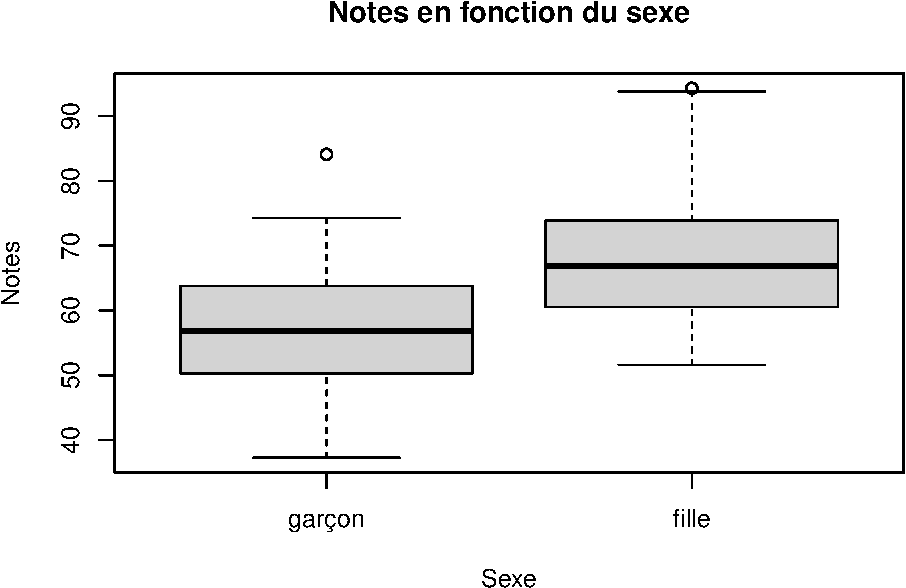
\includegraphics{_main_files/figure-latex/unnamed-chunk-50-1.pdf}
Ici, R traite la variable \emph{sexe} comme un facteur, c'est-à-dire comme une variable qui distingue différents états qui n'ont pas d'ordonnancement numérique. Pour cette raison, la fonction \emph{plot()} nous donne automatiquement un diagramme en boîte à moustache (c'est le nom!) puisque cela fait plus de sens pour des variables dichotomiques qui marquent des états distincts. Il demeure que cette variable est mathématiquement traitée comme si fille=1 et garçon = 0. Voyons ce qu'une telle figure donnerait si R «pense» que la variable est numérique.

\begin{Shaded}
\begin{Highlighting}[]
\CommentTok{\# La variable fille est utilisée ici plutôt que sexe parce que cette }
\CommentTok{\# variable est enregistrée dans R comme une variable de format numérique.}
\CommentTok{\# R la traite donc comme telle. Cependant, gardez bien à l\textquotesingle{}esprit que }
\CommentTok{\# cela revient mathématiquement au même. }
\FunctionTok{plot}\NormalTok{(fille, notes, }\AttributeTok{main=}\StringTok{"Notes en fonction du sexe"}\NormalTok{, }
    \AttributeTok{xlab=}\StringTok{"Sexe (garçon = 0, fille = 1)"}\NormalTok{, }\AttributeTok{ylab=}\StringTok{"Notes"}\NormalTok{, }\AttributeTok{pch=}\DecValTok{19}\NormalTok{, }\AttributeTok{data=}\NormalTok{data,}
    \FunctionTok{abline}\NormalTok{(m1))}
\end{Highlighting}
\end{Shaded}

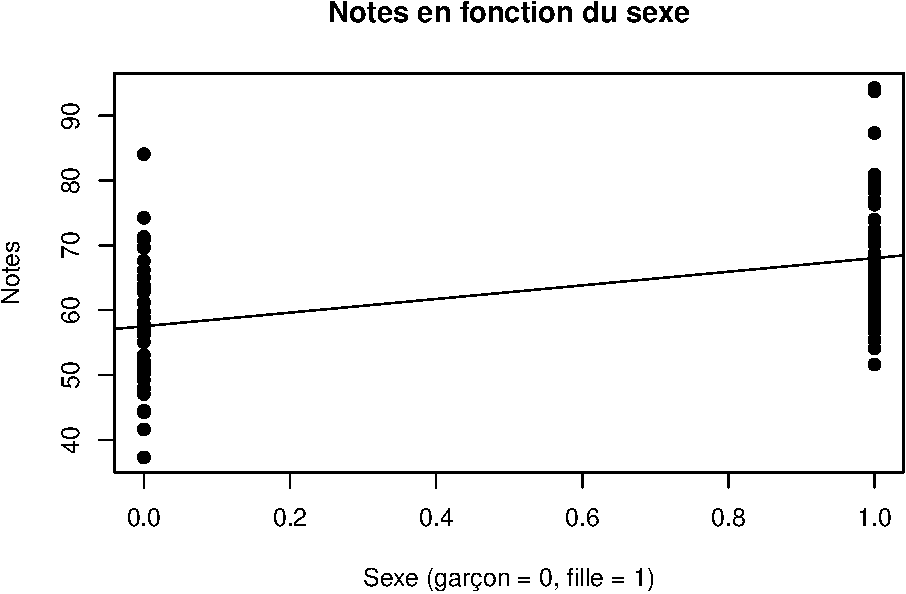
\includegraphics{_main_files/figure-latex/unnamed-chunk-51-1.pdf}
Chaque point est un individu. S'il s'agit d'un garçon, le point est à gauche (à 0) sur l'axe des x, alors qu'il est à droite (à 1) s'il s'agit d'une fille. Il n'y a personne au milieu puisqu'un élève est soit un garçon, soit une fille (raison pour laquelle cette variable est normalement traitée comme un facteur). La hauteur du point nous indique la note obtenue par l'élève. La ligne est l'équation de régression. La distance entre chaque point individuel et la ligne est l'erreur \(e_i\), c'est-à-dire ce qui n'est pas décrit parfaitement par notre équation (la ligne). Nous appelons aussi souvent cette erreur les «résidus».

L'intercept \emph{a} est la valeur moyenne de notre variable dépendante lorsque notre variable dépendante \emph{sexe} = 0. Autrement dit, \emph{a} est ici la note moyenne des garçons, soit 57.5282439. La valeur du coefficient de régression \(\beta\) (prononcé beta) nous indique le mouvement moyen de notre variable dépendante \emph{y} lorsque notre variable dépendante \emph{x} augmente de 1 unité. Dans le cas qui nous occupe, «augmenter» de 1 unité signifie être une fille plutôt qu'un garçon. Vous voyez donc que même si \(1>0\) alors que les filles ne peuvent pas être considérées «plus» que les garçons, cela ne fait pas réellement de différence mathématiquement puisqu'une unité peut ici être interprétée comme distinguant ces états qui n'ont pas d'ordonnancement hiérarchique. \emph{Cela n'est cependant vrai que pour les variables dichotomiques}, qui sont un cas particulier des \emph{variables nominales}\footnote{Les variables dichotomiques sont un cas particulier des \emph{variables nominales}. Comme les variables dichotomiques, les variables nominales distinguent des états différents qui ne peuvent être ordonnancés hiérarchiquement, mais elles comportent plus de deux possibilités. Un exemple de variable nominale est le choix de vote : PLQ, PQ, CAQ, QS. Ce sont là quatre possibilités distinctes qui ne peuvent être ordonnancées hiérarchiquement. Lorsque l'on veut utiliser une telle variable comme variable indépendante dans une régression, on ne peut pas laisser une telle variable dans un format numérique comme PLQ=1, PQ=2, CAQ=3 et QS=4 parce qu'il n'y a alors aucun moyen de distinguer mathématiquement qu'une unité de cette variable équivaut seulement à un état différent. Il faut alors «dichotomiser» toutes les options (par exemple : PLQ = 1, autres = 0; PQ = 0, autres = 0, etc.) et laisser une catégorie de référence à partir de laquelle les autres options seront interprétées. Nous y reviendrons plus tard. Ceci étant, R peut enregistrer des variables en différents formats, notamment en format numérique et en «facteur» (fator en anglais). Une variable en facteur est une variable qui distingue différents états qui ne sont pas hiérarchisés numériquement, comme le sexe ou le choix de vote. Lorsqu'une variable est enregistrée comme facteur, R dichotomisera automatiquement cette variable lorsqu'elle sera utilisée comme variable indépendante dans un modèle. Vous remarquerez que dans les modèles, j'ai utilisé la variable \emph{sexe} qui est enregistrée dans R comme facteur, plutôt que la variable \emph{fille} qui est enregistrée comme étant numérique. Puisqu'il s'agit d'une variable dichotomique, cela revient mathématiquement au même, mais cela a l'avantage de faciliter la création de certains graphiques. Si la variable sexe avait eu 3 catégories (disons garçons, filles et autres), alors la variable numérique n'aurait pas été équivalente à la variable enregistrée en facteur et il aurait impérativement fallu utiliser la variable en facteur dans les modèles.}.

Ainsi, dans le cas qui nous occupe, notre modèle prévoit que la note moyenne des filles sera de \(a+\beta x\), soit de 57.5282439 + 10.5077022= 68.0359461.

Rappelons-nous quelles étaient les moyennes des garçons et des filles dans notre tableau croisé :

\begin{Shaded}
\begin{Highlighting}[]
\NormalTok{data }\SpecialCharTok{\%\textgreater{}\%} 
  \FunctionTok{group\_by}\NormalTok{(sexe) }\SpecialCharTok{\%\textgreater{}\%} 
  \FunctionTok{summarise\_each}\NormalTok{ (}\FunctionTok{funs}\NormalTok{(mean) , }\AttributeTok{notes\_moy =}\NormalTok{ notes)}
\end{Highlighting}
\end{Shaded}

\begin{verbatim}
## # A tibble: 2 x 2
##   sexe   notes_moy
##   <fct>      <dbl>
## 1 garçon      57.5
## 2 fille       68.0
\end{verbatim}

Nous constatons que les chiffres sont très exactement les mêmes. La valeur de l'intercept \emph{a} est égal à la moyenne des garçons ( c'est-à-dire quand le sexe = 0), alors que \(a+\beta x\) est égal à la moyenne des filles. Inversement, nous pourrions aussi dire que dans ce cas, la valeur du \(\beta\) est tout simplement la différence de moyenne entre les garçons et les filles, soit 68.03595 - 57.52824 = 10.50771. Vous voyez donc que notre modèle de régression n'a rien de magique, il \emph{décrit} tout simplement nos données.

Vous comprendez aussi que lorsque nous proposons l'équation \(y_i=a+\beta x_i + e_i\), ne sommes absolument pas en train de dire que les notes des élèves de notre cours de pétanque obéissent à une sorte de loi immuable de l'univers. Nous disons simplement que les notes de nos élèves varient autour d'une certaine valeur \(a\) et qu'elles ont tendance à être différentes (une différence moyenne de valeur \(\beta\)) en fonction du sexe des élèves. Nous ne savons pas si le sexe des élèves est la \emph{cause} de la variation des notes, mais nous constatons tout simplement que, dans nos données, les filles ont tendance à avoir de meilleures notes que les garçons. Plutôt que de décrire les données en donnant la moyenne des garçons et des filles séparément (décrire les données avec deux chiffres, les moyennes par groupe), nous avons simplement proposé une équation qui est équivalente.

\hypertarget{la-ruxe9gression-linuxe9aire-simple-avec-une-variable-continue}{%
\section{La régression linéaire simple avec une variable continue}\label{la-ruxe9gression-linuxe9aire-simple-avec-une-variable-continue}}

Jusqu'ici, notre variable dépendante a été dichotomique (garçon = 0, fille =1). Un coefficient de régression nous donne le mouvement dans la variable dépendante associée \emph{au mouvement d'une unité de la variable indépendante}. Les coefficients des variables dichotomiques sont plus «faciles» à interpréter puisqu'ils s'interprètent tout simplement comme le fait d'être dans un groupe plutôt que dans l'autre, ou la différence entre les deux groupes. Cependant, nous utilisons aussi régulièrement des variables continues, donc des variables dont les valeurs \emph{sont ordonnancées hiérarchiquement} et dont \emph{l'unité de mesure peut être considérée comme standard}.\footnote{Comme nous l'avons vu plus haut, il existe aussi \emph{les variables ordinales} qui sont ordonnancées hiérarchiquement, mais qui ne sont pas mesurées sur une unité standard. La différence entre les variables numériques et la variable ordinale n'est pas toujours claire et il faut donc faire preuve de jugement lorsque l'on procède à l'analyse statistique. Lorsque l'on détermine qu'une variable doit être traitée comme étant ordinale, elle doit être dichotomisée, comme les variables nominales. Voir la note {[}\^{}3{]} pour plus de détails.} Faisons donc un modèle similaire, mais en utilisant cette fois le nombre d'heures d'étude de nos élèves.

Commençons par visualiser de quoi ont l'air les données en fonction du nombre d'heures étudiées par semaine.

\begin{Shaded}
\begin{Highlighting}[]
\FunctionTok{plot}\NormalTok{(heures.etude, notes, }\AttributeTok{main=}\StringTok{"Notes en fonction des heures étudiées"}\NormalTok{,}
     \AttributeTok{xlim=}\FunctionTok{c}\NormalTok{(}\DecValTok{0}\NormalTok{, }\DecValTok{10}\NormalTok{), }\AttributeTok{ylim=}\FunctionTok{c}\NormalTok{(}\DecValTok{20}\NormalTok{, }\DecValTok{100}\NormalTok{),}
    \AttributeTok{xlab=}\StringTok{"Heures d\textquotesingle{}étude"}\NormalTok{, }\AttributeTok{ylab=}\StringTok{"Notes"}\NormalTok{, }\AttributeTok{pch=}\DecValTok{19}\NormalTok{, }\AttributeTok{data=}\NormalTok{data)}
\end{Highlighting}
\end{Shaded}

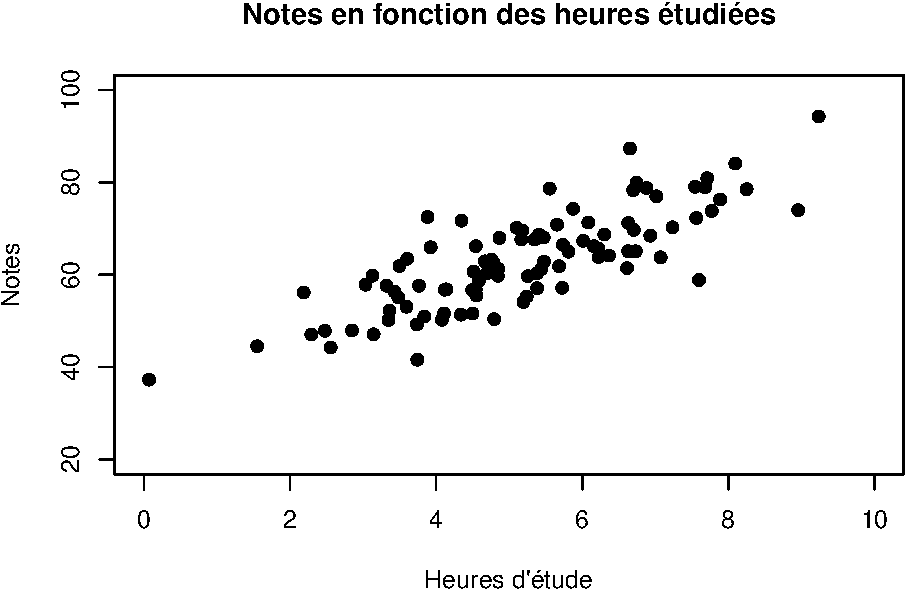
\includegraphics{_main_files/figure-latex/unnamed-chunk-53-1.pdf}

Visuellement, il est assez clair que ceux qui étudient davantage ont de meilleures notes. De manière analogue à ce que nous faisons lorsque nous calculons une moyenne pour synthétiser une vaste quantité d'information, nous pourrions ici vouloir résumer le plus succinctement possible ce que nous observons chez ces 100 élèves. Bien entendu, chaque individu est intéressant, mais nous nous intéressons ici aux notes moyennes des élèves en fonction des heures d'étude. C'est précisément ce que calcule la régression linéaire.

\begin{Shaded}
\begin{Highlighting}[]
\NormalTok{m2 }\OtherTok{\textless{}{-}} \FunctionTok{lm}\NormalTok{(notes}\SpecialCharTok{\textasciitilde{}}\NormalTok{heures.etude) }\CommentTok{\# Crée l\textquotesingle{}objet m2 qui contient les résultats}
\CommentTok{\# d\textquotesingle{}un modèle linéaire (fonction lm() pour "linear model") dans lequel }
\CommentTok{\# la variable note est une fonction (\textasciitilde{}) de la variable heure.etude. }
\FunctionTok{summary}\NormalTok{(m2) }\CommentTok{\# Pour voir les résultats contenus dans l\textquotesingle{}objet m2.}
\end{Highlighting}
\end{Shaded}

\begin{verbatim}
## 
## Call:
## lm(formula = notes ~ heures.etude)
## 
## Residuals:
##      Min       1Q   Median       3Q      Max 
## -16.3271  -3.7251  -0.6483   4.1989  16.8874 
## 
## Coefficients:
##              Estimate Std. Error t value Pr(>|t|)    
## (Intercept)    36.981      1.957   18.90   <2e-16 ***
## heures.etude    5.030      0.353   14.25   <2e-16 ***
## ---
## Signif. codes:  0 '***' 0.001 '**' 0.01 '*' 0.05 '.' 0.1 ' ' 1
## 
## Residual standard error: 6.227 on 98 degrees of freedom
## Multiple R-squared:  0.6744, Adjusted R-squared:  0.6711 
## F-statistic:   203 on 1 and 98 DF,  p-value: < 2.2e-16
\end{verbatim}

Les résultats de notre modèle nous indiquent que chaque heure d'étude supplémentaire est \emph{en moyenne} associée à des notes plus élevées de 5.0295675. Un élève qui n'a pas étudié obtient donc, en moyenne, la valeur de l'intercept \emph{a}, soit de 36.9810477. Un élève qui a étudié 1 heure obtient en moyenne \(a + \beta \times 1\), soit 36.9810477 + 5.0295675 = 42.0106152. Un élève qui a étudié 2 heures obtient en moyenne \(a + \beta \times 2\), soit 36.9810477 + 5.0295675 X 2 = 47.0401827. Un élève qui a étudié 8 heures obtient en moyenne \(a + \beta \times 8\), soit 36.9810477 + 5.0295675 X 8 = 77.2175877.

Voici notre ligne de régression par rapport à nos points. Si vous observez où passe cette ligne, vous constaterez qu'elle est directement sur les «valeurs prédites» que nous avons calculées au paragraphe précédent.

\begin{Shaded}
\begin{Highlighting}[]
\FunctionTok{plot}\NormalTok{(heures.etude, notes, }\AttributeTok{main=}\StringTok{"Notes en fonction des heures étudiées"}\NormalTok{,}
     \AttributeTok{xlim=}\FunctionTok{c}\NormalTok{(}\DecValTok{0}\NormalTok{, }\DecValTok{10}\NormalTok{), }\AttributeTok{ylim=}\FunctionTok{c}\NormalTok{(}\DecValTok{20}\NormalTok{, }\DecValTok{100}\NormalTok{),}
    \AttributeTok{xlab=}\StringTok{"Heures d\textquotesingle{}étude"}\NormalTok{, }\AttributeTok{ylab=}\StringTok{"Notes"}\NormalTok{, }\AttributeTok{pch=}\DecValTok{19}\NormalTok{, }\AttributeTok{data=}\NormalTok{data,}
    \FunctionTok{abline}\NormalTok{(}\FunctionTok{lm}\NormalTok{(notes}\SpecialCharTok{\textasciitilde{}}\NormalTok{heures.etude)))}
\end{Highlighting}
\end{Shaded}

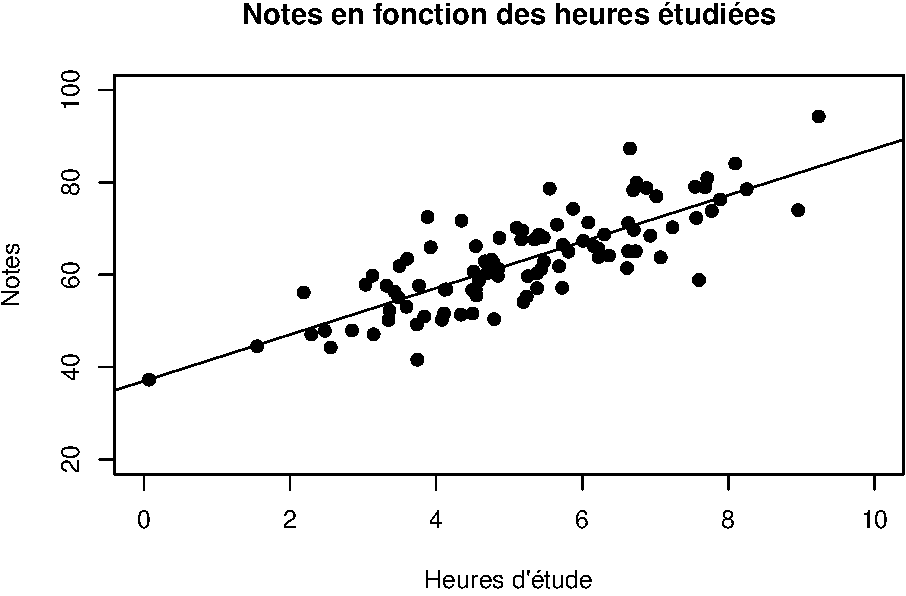
\includegraphics{_main_files/figure-latex/unnamed-chunk-56-1.pdf}

Tout comme une moyenne résume en un seul chiffre la valeur centrale d'une variable, l'équation de régression linéaire résume en quelques coefficients la relation entre deux ou plusieurs variables. Cette équation correspond tout simplement à une ligne que l'on trace au milieu des points. Encore une fois, l'équation ne signifie absolument pas que le phénomène qui nous intéresse obéit à une loi immuable de l'univers. L'équation ne fait que \emph{résumer} et \emph{décrire} ce que nous observons dans les données.

La ligne de régression est calculée de manière à \emph{minimiser} la \emph{somme des erreurs au carré}. La somme des erreurs au carré réfère à la somme totale des \emph{résidus}, soit la distance de chaque point par rapport à la ligne de régression. Cette distance est ensuite mise au carré. Puis, nous faisons la même chose pour tous les points et nous additionnons ces distances pour obtenir la \emph{somme des erreurs au carré}. Le fait que la régression linéaire minimise cette somme est importante parce que cela veut dire qu'il n'existe pas de meilleure ligne qui puisse décrire ces données. Il n'y a pas de meilleure ligne parce que c'est celle qui est le plus près possible de tous les points à la fois. Vous vous rappelez peut-être que nous disions plus haut que la moyenne a une propriété similaire : une moyenne minimise la somme des \emph{écarts à la moyenne au carré}. Le principe est ici le même.

Évidemment, l'équation de régression ne décrit pas parfaitement la relation, il y a des points qui ne sont pas directement sur la ligne (il y a des «résidus», des écarts entre chaque point et la ligne), mais souvenez-vous qu'il en était de même pour la moyenne d'un groupe et chaque individu. La régression résume la relation entre nos deux variables de manière à ce que nous soyons capables de manipuler cette information. Encore une fois, il n'y a rien de magique à cela, nous ne faisons que \emph{décrire} nos données à l'aide d'une équation. J'espère qu'au passage vous commencez à arrêter de faire de l'angoisse devant les équations!

\hypertarget{la-ruxe9gression-linuxe9aire-avec-plusieurs-variables-induxe9pendantes}{%
\section{La régression linéaire avec plusieurs variables indépendantes}\label{la-ruxe9gression-linuxe9aire-avec-plusieurs-variables-induxe9pendantes}}

Jusqu'à présent, nous n'avons utilisé qu'une seule variable indépendante à la fois. Nous avons vu qu'une régression linéaire avec une variable dichotomique comme prédicteur nous permettait facilement de retrouver les moyennes de nos deux groupes (garçons et filles). Nous avons aussi vu comment une régression similaire qui utilise une variable continue comme prédicteur nous permet aussi de résumer simplement le lien entre une unité de ce prédicteur et la variable dépendante. Nous pourrions cependant nous intéresser au lien spécifique d'une, mais variable en tenant compte d'une ou de plusieurs autres variables. C'est ce que permet la régression multiple.

Cela est important parce que, si par exemple les filles ont tendance à étudier plus d'heures que les garçons et que le nombre d'heures passées à étudier est lié aux notes obtenues, on peut alors se demander si c'est réellement le fait d'être une fille qui fait en sorte qu'elles ont de meilleures notes, ou si cela est simplement lié au fait qu'elles étudient plus. Le problème que nous nous posons ici est similaire à l'exemple de l'ampleur des dégâts lors d'un incendie, du nombre de pompiers qui le combattent et de l'intensité d'un incendie donné plus haut. Nous nous demandons si la relation entre l'une ou autre de nos variables d'intérêts est réelle ou fallacieuse.

Voyons dans nos données le nombre d'heures d'étude en fonction du sexe.

\begin{Shaded}
\begin{Highlighting}[]
\CommentTok{\# Tableau croisé des heures d\textquotesingle{}étude moyennes selon le sexe}
\NormalTok{data }\SpecialCharTok{\%\textgreater{}\%} 
  \FunctionTok{group\_by}\NormalTok{(sexe) }\SpecialCharTok{\%\textgreater{}\%} 
  \FunctionTok{summarise\_each}\NormalTok{ (}\FunctionTok{funs}\NormalTok{(mean) , }\AttributeTok{h.etude\_moy =}\NormalTok{ heures.etude)}
\end{Highlighting}
\end{Shaded}

\begin{verbatim}
## # A tibble: 2 x 2
##   sexe   h.etude_moy
##   <fct>        <dbl>
## 1 garçon        4.36
## 2 fille         5.96
\end{verbatim}

Nous voyons dans nos données que les filles étudient davantage. Les garçons étudient en moyenne 4.36 heures alors que les filles étudient 5.95 heures. Ainsi, on pourra se demander si, dépendamment du nombre d'heures étudiées, les filles obtiennent quand même de meilleurs résultats. Entre d'autres mots, nous pouvons nous demander si une fille qui a étudié 5 heures a en moyenne la même note qu'un garçon qui a étudié lui aussi 5 heures, ou si elle a quand même une meilleure note du simple fait d'être une fille. Pour répondre à cette question, nous allons estimer l'équation de régression linéaire suivante :
\[ Y =  a + \beta_1X_1 + \beta_2X_2 + e  \]
Ici, \emph{a} est encore une fois l'intercept, \(\beta_1\) est le coefficient de régression de la variable dichotomique \emph{sexe}, \(\beta_2\) est le coefficient de régression de la variable continue \_heures.etude et \(e\) est le terme d'erreur individuel, ou ce qui n'est pas expliqué par nos autres variables. Pour aider le lecteur, on pourrait écrire l'équation comme suit :
\[ Y =  a + \beta_1 sexe + \beta_2 heure.etude + e  \]
\(\beta_1\) et \(\beta_2\) sont indicés de 1 et 2 pour bien les distinguer, mais les autres variables ne sont pas indicées de \emph{i} tout simplement parce que l'indice est sous-entendu et ne porte pas à confusion. Il est évident que le sexe et les heures d'étude varient entre les individus.

Estimons maintenant cette équation dans R.

\begin{Shaded}
\begin{Highlighting}[]
\NormalTok{m3 }\OtherTok{\textless{}{-}} \FunctionTok{lm}\NormalTok{(notes }\SpecialCharTok{\textasciitilde{}}\NormalTok{ sexe }\SpecialCharTok{+}\NormalTok{ heures.etude) }\CommentTok{\# Créer l\textquotesingle{}objet m1 qui contient}
\CommentTok{\# les résultats \# d\textquotesingle{}un modèle linéaire (fonction lm() pour "linear model")}
\CommentTok{\# dans lequel la variable note est une fonction (\textasciitilde{}) du sexe }
\CommentTok{\# ET de heure.etude.}
\FunctionTok{summary}\NormalTok{(m3)}
\end{Highlighting}
\end{Shaded}

\begin{verbatim}
## 
## Call:
## lm(formula = notes ~ sexe + heures.etude)
## 
## Residuals:
##      Min       1Q   Median       3Q      Max 
## -13.6705  -4.2615  -0.6981   3.9705  16.0712 
## 
## Coefficients:
##              Estimate Std. Error t value Pr(>|t|)    
## (Intercept)   37.3057     1.9227  19.403   <2e-16 ***
## sexefille      3.1023     1.3758   2.255   0.0264 *  
## heures.etude   4.6372     0.3872  11.977   <2e-16 ***
## ---
## Signif. codes:  0 '***' 0.001 '**' 0.01 '*' 0.05 '.' 0.1 ' ' 1
## 
## Residual standard error: 6.101 on 97 degrees of freedom
## Multiple R-squared:  0.6906, Adjusted R-squared:  0.6843 
## F-statistic: 108.3 on 2 and 97 DF,  p-value: < 2.2e-16
\end{verbatim}

Nos résultats nous indiquent donc qu'indépendamment du nombre d'heures d'étude, les filles ont en moyenne des notes de 3.1023461 points supérieurs aux garçons. Par ailleurs, en tenant compte de la différence entre les garçons et les filles, chaque heure d'étude supplémentaire apporte en moyenne 4.6372014 points de plus.
À partir de ces résultats, il est possible d'estimer la note d'un garçon qui a étudié 5 heures en complétant simplement notre équation :
\[Y =  a + \beta_1 sexe + \beta_2 heure.etude\]
\[Y =  37.3057061 + 3.1023461 sexe + 4.6372014 heure.etude\]
\[Y =  37.3057061 + 3.1023461 \times 0 + 4.6372014 \times 5\]
En résolvant l'équation, on arrive à 60.4917131. Si au lieu d'un garçon on s'intéressait à la note moyenne d'une fille qui a elle aussi étudié 5 heures, il suffit encore de résoudre l'équation en ajustant les chiffres.
\[Y =  37.3057061 + 3.1023461 \times 1 + 4.6372014 \times 5\]
Nous obtenons alors 63.5940592. La différence entre le garçon et la fille qui ont étudié le même nombre d'heures (63.5940592 -60.4917131 = 3.1023461) équivaut alors précisément à notre coefficient \(\beta_1\) de 3.1023461.

Il peut être difficile de visualiser des résultats de régression multiple sur une surface en deux dimensions. Nous pourrions faire un graphique en trois dimensions, mais la surface sur laquelle il est projeté (du papier ou un écran) demeure bidimensionnelle. La meilleure manière de s'y prendre est d'ajouter de la couleur.

\begin{Shaded}
\begin{Highlighting}[]
\FunctionTok{library}\NormalTok{(ggplot2) }\CommentTok{\# charger ggplot2, super package pour les graphiques}
\CommentTok{\# Notez que le package ggplot2 permet l\textquotesingle{}ajout d\textquotesingle{}un +}
\CommentTok{\# en fin de ligne pour lui dire qu\textquotesingle{}une autre ligne ajoutant des }
\CommentTok{\# éléments à la figure suit. Un + n\textquotesingle{}est pas nécessaire si }
\CommentTok{\# une parenthèse est déjà ouverte et n\textquotesingle{}a pas encore été fermée.}

\CommentTok{\# Notez aussi comment la syntaxe est écrite. Les indentations n\textquotesingle{}ont aucun}
\CommentTok{\# effet sur le résultat, mais ils améliorent la lisibilité. Il est }
\CommentTok{\# beaucoup plus facile de lire une longue parenthèse dans une }
\CommentTok{\# syntaxe lorsque celle{-}ci est indentée à partir de la première}
\CommentTok{\# parenthèse. Voir après «theme(». Toutes les options dans cette}
\CommentTok{\# parenthèse sont indentées sous celle{-}ci. Cela est simplement une }
\CommentTok{\# question de lisibilité. Le tout pourrait être écrit en une seule ligne}
\CommentTok{\# interminable (et difficile à lire). Mieux vaut l\textquotesingle{}écrire en plusieurs}
\CommentTok{\# lignes. }
\FunctionTok{ggplot}\NormalTok{(data, }\FunctionTok{aes}\NormalTok{(heures.etude, notes, }\AttributeTok{colour=}\NormalTok{sexe)) }\SpecialCharTok{+} 
  \FunctionTok{ggtitle}\NormalTok{(}\StringTok{"Notes des élèves en fonction du sexe et des heures étudiées"}\NormalTok{) }\SpecialCharTok{+}
  \FunctionTok{xlim}\NormalTok{(}\DecValTok{0}\NormalTok{, }\DecValTok{10}\NormalTok{) }\SpecialCharTok{+}
  \FunctionTok{ylim}\NormalTok{(}\DecValTok{30}\NormalTok{, }\DecValTok{100}\NormalTok{) }\SpecialCharTok{+}
  \FunctionTok{ylab}\NormalTok{(}\StringTok{"Notes"}\NormalTok{) }\SpecialCharTok{+} 
  \FunctionTok{xlab}\NormalTok{(}\StringTok{"Heures d\textquotesingle{}étude"}\NormalTok{) }\SpecialCharTok{+}
  \FunctionTok{geom\_smooth}\NormalTok{(}\AttributeTok{method =}\NormalTok{ lm, }\AttributeTok{se=}\ConstantTok{FALSE}\NormalTok{, }\AttributeTok{fullrange=}\ConstantTok{TRUE}\NormalTok{) }\SpecialCharTok{+} \CommentTok{\# lignes de régression}
  \FunctionTok{geom\_point}\NormalTok{() }\SpecialCharTok{+} \CommentTok{\# les points individuels}
  \FunctionTok{theme}\NormalTok{(}\AttributeTok{panel.grid.major =} \FunctionTok{element\_blank}\NormalTok{(), }\CommentTok{\# Ce qui suit est esthétique}
        \AttributeTok{panel.grid.minor =} \FunctionTok{element\_blank}\NormalTok{(),}
        \AttributeTok{panel.background =} \FunctionTok{element\_blank}\NormalTok{(), }
        \AttributeTok{axis.line =} \FunctionTok{element\_line}\NormalTok{(}\AttributeTok{colour =} \StringTok{"black"}\NormalTok{),}
        \AttributeTok{panel.border =} \FunctionTok{element\_rect}\NormalTok{(}\AttributeTok{fill=}\ConstantTok{NA}\NormalTok{,}\AttributeTok{color=}\StringTok{"black"}\NormalTok{,}
                                    \AttributeTok{size=}\FloatTok{0.3}\NormalTok{, }\AttributeTok{linetype=}\StringTok{"solid"}\NormalTok{)}
\NormalTok{        )}
\end{Highlighting}
\end{Shaded}

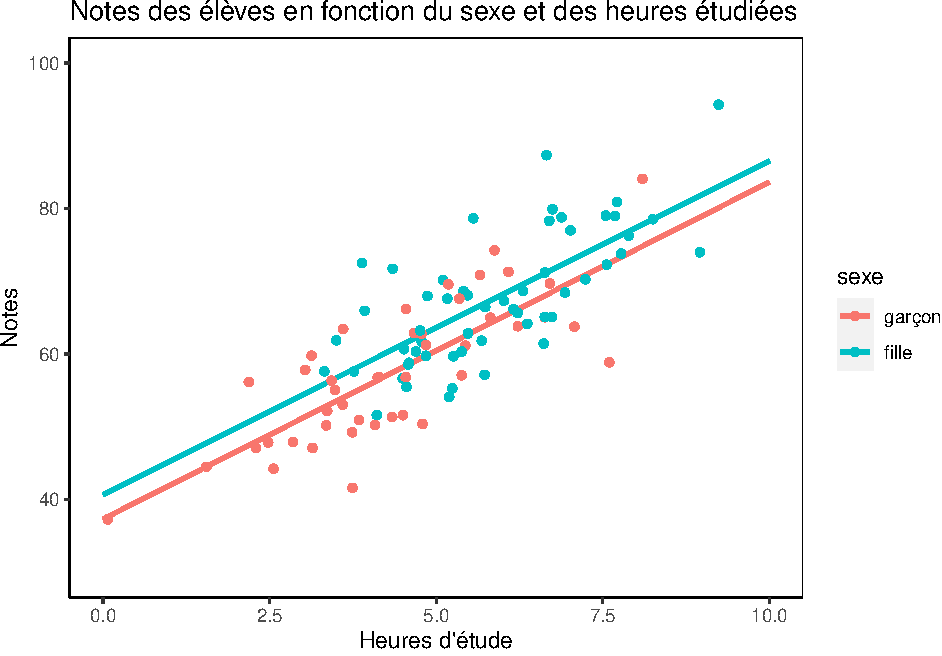
\includegraphics{_main_files/figure-latex/unnamed-chunk-60-1.pdf}

Nous voyons dans cette figure le résultat de notre régression. Le bleu correspond aux filles et le rouge aux garçons. Nous voyons que leurs droites de régression ont la même pente (\(\beta_2\)) et augmentent de 4.6372014 pour chaque heure d'étude supplémentaire. Cependant, la droite des filles est plus élevée de 3.1023461 par rapport à celle des garçons (\(\beta_1\)) qui débute à l'intercept \emph{a}, soit à 37.3057061. En observant les points bleus, nous voyons qu'il n'y a aucune fille dans nos données qui a étudié 0 heure (en fait, aucune fille n'a étudié moins de 3 heures), mais nos résultats nous permettent \emph{d'estimer} la note éventuelle d'une fille qui n'aurait pas étudié. Encore une fois, on trouverait cette valeur précise en résolvant notre équation de régression :

\[Y =  37.3057061 + 3.1023461 \times 1 + 4.6372014 \times 0\]
Puisque les heures étudiées sont de 0 (4.6372014 X 0 = 0), cela se simplifie en :
\[Y =  37.3057061 + 3.1023461 \times 1\]
Ce qui nous donne 37.3057061. Évidemment, il faut être prudent lorsque nous prédisons de la sorte des valeurs en dehors de nos données, mais l'objectif est ici de vous montrer la logique.

\hypertarget{la-ruxe9gression-linuxe9aire-un-exemple-avec-des-donnuxe9es-ruxe9elles}{%
\section{La régression linéaire, un exemple avec des données réelles}\label{la-ruxe9gression-linuxe9aire-un-exemple-avec-des-donnuxe9es-ruxe9elles}}

Nous avons jusqu'ici utilisé des données fictives que nous avons nous-mêmes créées afin de mieux comprendre l'outil de la régression. Cependant, dans la vraie vie nous utilisons évidemment des «vraies» données. Nous allons ici voir comment une analyse de régression linéaire se fait «dans la vraie vie». Ce faisant, nous verrons qu'il faut préalablement «nettoyer» un peu les données en recodant convenablement les variables avant de procéder. J'utiliserai ici les données des \href{https://ces-eec.arts.ubc.ca/french-section/enquetes/}{\emph{Études électorales canadiennes}} de 2015. Ces données sont produites lors de chaque élection fédérale et elles sont rendues disponibles gratuitement sur le site internet de l'étude.

Comme nous l'avons fait plus haut, chargeons maintenant ces données.

\begin{Shaded}
\begin{Highlighting}[]
\CommentTok{\#rm(list = ls())}

\CommentTok{\# Pour charger des données du format Stata, nous avons besoin du package }
\CommentTok{\# "readstata13" qui inclut les fonctions de transformation nécessaires. }
\CommentTok{\#library(readstata13)}

\CommentTok{\# Chargeons les données.}
\CommentTok{\#ces15 \textless{}{-} read.dta13("CES2015{-}phone{-}release/CES2015\_CPS{-}PES{-}MBS\_complete{-}v2.dta")}

\FunctionTok{library}\NormalTok{(haven)}
\NormalTok{ces15 }\OtherTok{\textless{}{-}} \FunctionTok{read\_sav}\NormalTok{(}\StringTok{"data/CES2015\_CPS{-}PES{-}MBS\_complete{-}v2.sav"}\NormalTok{)}
\end{Highlighting}
\end{Shaded}

Nous nous intéresserons à l'appréciation de Justin Trudeau et nous utiliserons ce que nous appelons sa «mesure thermométrique». Nous demandons simplement aux répondants de dire, sur une échelle de 0 à 100 où 0 veut dire qu'ils ne l'aiment pas du tout et 100 veut dire qu'ils l'aiment beaucoup. La question est formulée comme suit:

« Maintenant les chefs de partis. Utiliser la même échelle, où zéro veut dire que vous N'AIMEZ VRAIMENT PAS DU TOUT un chef, et cent veut dire que vous L'AIMEZ VRAIMENT BEAUCOUP.

Que pensez\_vous de JUSTIN TRUDEAU?»

Dans les données, cette variable est nommée «CPS15\_24», qui est un titre très informatif\ldots{} Voyons voir de quoi la variable a l'air.

\begin{Shaded}
\begin{Highlighting}[]
\FunctionTok{summary}\NormalTok{(ces15}\SpecialCharTok{$}\NormalTok{CPS15\_24)}
\end{Highlighting}
\end{Shaded}

\begin{verbatim}
##    Min. 1st Qu.  Median    Mean 3rd Qu.    Max.    NA's 
##       0      35      60     109      75     999      20
\end{verbatim}

\begin{Shaded}
\begin{Highlighting}[]
\CommentTok{\# Faire un histograme}
\FunctionTok{hist}\NormalTok{(ces15}\SpecialCharTok{$}\NormalTok{CPS15\_24)}
\end{Highlighting}
\end{Shaded}

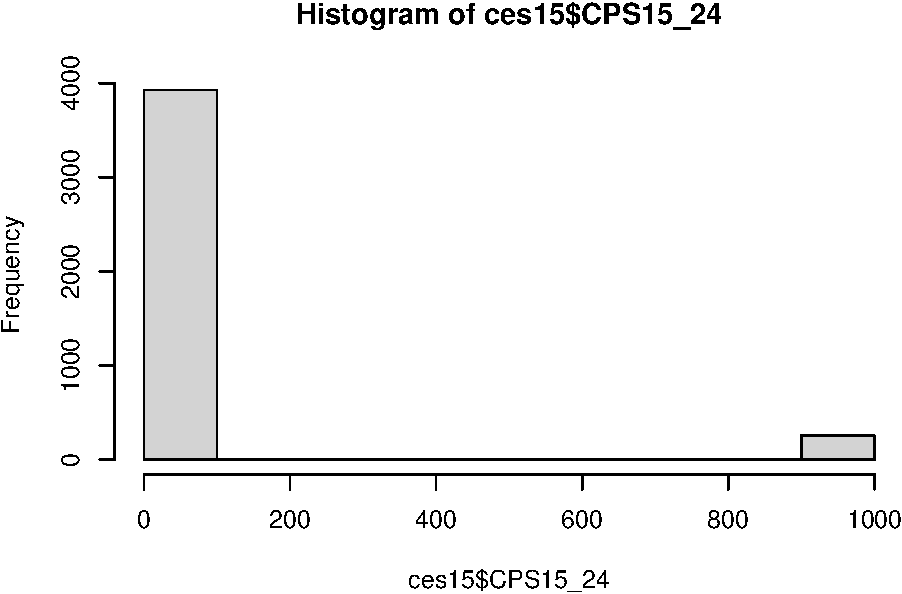
\includegraphics{_main_files/figure-latex/unnamed-chunk-62-1.pdf}

On remarque que pour une variable qui est censée aller de 0 à 100, nous avons des valeurs étrangement élevées. Cela arrive fréquemment. Un coup d'oeil à la documentation fournie avec les données nous indique que les «Ne sais pas» ont été codés 998, et les «Refus» ont été codés 999. R assume que ces réponses sont «valables» et il faut donc nettoyer cette variable en codant ces réponses de manières appropriées. Ici, nous traiterons ces réponses comme des valeurs manquantes, qui sont codées dans R par «NA».

\begin{Shaded}
\begin{Highlighting}[]
\NormalTok{ces15}\SpecialCharTok{$}\NormalTok{thermo.trudeau }\OtherTok{\textless{}{-}} \FunctionTok{as.numeric}\NormalTok{(ces15}\SpecialCharTok{$}\NormalTok{CPS15\_24) }\CommentTok{\# Créé la variable }
\CommentTok{\# "thermo.truceau" dans la matrice ces15 en copiant le contenu }
\CommentTok{\# de la variable CPS15\_24 dans la matrice data.ces}
\CommentTok{\# J\textquotesingle{}ai ici utilisé l\textquotesingle{}option as.numeric() parce que CPS15\_24 était}
\CommentTok{\# encodé dans un format "labelled" et nous préférons ici avoir }
\CommentTok{\# simplement les valeurs numériques. }

\CommentTok{\# Recoder les valeurs de la variable thermo.trudeau pour que ce qui }
\CommentTok{\# est plus grand que 100 soit transormé en valeur manquante.}
\NormalTok{ces15}\SpecialCharTok{$}\NormalTok{thermo.trudeau[ces15}\SpecialCharTok{$}\NormalTok{thermo.trudeau }\SpecialCharTok{\textgreater{}} \DecValTok{100}\NormalTok{] }\OtherTok{\textless{}{-}} \ConstantTok{NA}

\CommentTok{\# Faire un histogramme et préciser les titres}
\FunctionTok{hist}\NormalTok{(ces15}\SpecialCharTok{$}\NormalTok{thermo.trudeau,}
  \AttributeTok{main =} \StringTok{"Themomètre sur l\textquotesingle{}appéciation de Justin Trudeau"}\NormalTok{,}
  \AttributeTok{xlab =} \StringTok{"Score thermométrique"}\NormalTok{,}
  \AttributeTok{ylab =} \StringTok{"Fréquence"}
\NormalTok{)}
\end{Highlighting}
\end{Shaded}

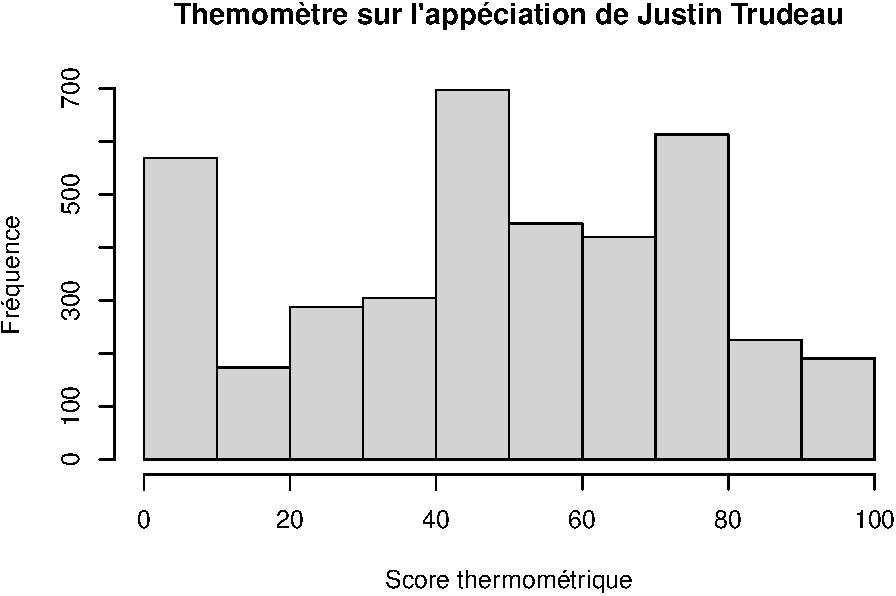
\includegraphics{_main_files/figure-latex/unnamed-chunk-63-1.pdf}

\begin{Shaded}
\begin{Highlighting}[]
\CommentTok{\# On aurait pu faire la même chose sans placer la nouvelle variable}
\CommentTok{\# thermo.trudeau dans la matrice de données initiale ces15. }
\CommentTok{\# thermo.trudeau serait alors un nouvel objet en lui{-}même. Comme ceci:}

\NormalTok{thermo.trudeau }\OtherTok{\textless{}{-}}\NormalTok{ ces15}\SpecialCharTok{$}\NormalTok{CPS15\_24}
\NormalTok{thermo.trudeau[thermo.trudeau }\SpecialCharTok{\textgreater{}} \DecValTok{100}\NormalTok{] }\OtherTok{\textless{}{-}} \ConstantTok{NA}

\CommentTok{\# Cependant, il vaut souvent mieux garder les variables à l\textquotesingle{}intérieur}
\CommentTok{\# de matrices pour garder de l\textquotesingle{}ordre dans notre session. Éliminons }
\CommentTok{\# donc l\textquotesingle{}objet "thermo.trudeau" seul, et utilisons sa copie située dans}
\CommentTok{\# la matrice ces15}

\FunctionTok{rm}\NormalTok{(thermo.trudeau)}
\end{Highlighting}
\end{Shaded}

Imaginons maintenant que nous nous intéressions à la perception de Trudeau chez les répondants en fonction de leur niveau d'éducation. La variable d'éducation dans les données est nommée «CPS15\_79», encore une fois un nom très utile\ldots{}

\begin{Shaded}
\begin{Highlighting}[]
\FunctionTok{table}\NormalTok{(ces15}\SpecialCharTok{$}\NormalTok{CPS15\_79)}
\end{Highlighting}
\end{Shaded}

\begin{verbatim}
## 
##    1    2    3    4    5    6    7    8    9   10   11   98   99 
##    5   30   65  321  765  233  930  285 1007  360  165   11   25
\end{verbatim}

Encore une fois, cette variable a des codes étranges (98 et 99). Un coup d'oeil à la documentation nous informe sur comment cette variable a été codée:

Quel est le plus haut niveau d'éducation que vous avez complété?\\
1 aucune scolarité
2 quelques années à l'élémentaire\\
3 école élémentaire terminée
4 quelques années d'école secondaire
5 école secondaire terminée\\
6 quelques études au collège, au cégep, au collège classique
7 études terminées au collège, au cégep, au collège classique\\
8 quelques études universitaires\\
9 baccalauréat\\
10 maîtrise\\
11 diplôme professionnel ou doctorat
98 Ne sais pas
99 Refus

Nous devons donc encore une fois «nettoyer» cette variable, minimalement en recodeant les 98 et 99 en tant que valeurs manquantes.

\begin{Shaded}
\begin{Highlighting}[]
\NormalTok{ces15}\SpecialCharTok{$}\NormalTok{educ }\OtherTok{\textless{}{-}}\NormalTok{ ces15}\SpecialCharTok{$}\NormalTok{CPS15\_79 }\CommentTok{\# Je créé encore une fois une nouvelle variable}
\CommentTok{\# "educ" dans l\textquotesingle{}objet ces15qui est une copie de CPS15\_79. Elle aura un nom}
\CommentTok{\# plus informatif}
\NormalTok{ces15}\SpecialCharTok{$}\NormalTok{educ[ces15}\SpecialCharTok{$}\NormalTok{educ }\SpecialCharTok{\textgreater{}} \DecValTok{11}\NormalTok{] }\OtherTok{\textless{}{-}} \ConstantTok{NA} \CommentTok{\# Change les valeurs plus grandes que 11 pour NA}
\FunctionTok{table}\NormalTok{(ces15}\SpecialCharTok{$}\NormalTok{educ)}
\end{Highlighting}
\end{Shaded}

\begin{verbatim}
## 
##    1    2    3    4    5    6    7    8    9   10   11 
##    5   30   65  321  765  233  930  285 1007  360  165
\end{verbatim}

Nous pourrions maintenant vouloir une variable d'éducation qui regroupe certains niveaux d'études. Nous pourrions vouloir avoir quatre niveaux d'éducation plutôt que 11.

\begin{Shaded}
\begin{Highlighting}[]
\NormalTok{ces15}\SpecialCharTok{$}\NormalTok{educ.gp }\OtherTok{\textless{}{-}}\NormalTok{ ces15}\SpecialCharTok{$}\NormalTok{educ }\CommentTok{\# Copie la variable "educ" dans la nouvelle }
\CommentTok{\# variable "educ.gp"}

\NormalTok{ces15}\SpecialCharTok{$}\NormalTok{educ.gp }\OtherTok{\textless{}{-}} \FunctionTok{as.numeric}\NormalTok{(ces15}\SpecialCharTok{$}\NormalTok{educ.gp) }\CommentTok{\# Transfoirme en numérique pour éliminer les éléments liés à SPSS}

\CommentTok{\# Créé les différentes catégories}

\NormalTok{ces15}\SpecialCharTok{$}\NormalTok{educ.gp[ces15}\SpecialCharTok{$}\NormalTok{educ.gp }\SpecialCharTok{\textless{}} \DecValTok{5}\NormalTok{] }\OtherTok{\textless{}{-}} \StringTok{"Moins que secondaire"}
\NormalTok{ces15}\SpecialCharTok{$}\NormalTok{educ.gp[ces15}\SpecialCharTok{$}\NormalTok{educ.gp }\SpecialCharTok{==} \DecValTok{5}\NormalTok{] }\OtherTok{\textless{}{-}} \StringTok{"Secondaire complété"}
\NormalTok{ces15}\SpecialCharTok{$}\NormalTok{educ.gp[ces15}\SpecialCharTok{$}\NormalTok{educ.gp }\SpecialCharTok{\textgreater{}} \DecValTok{5} \SpecialCharTok{\&}\NormalTok{ ces15}\SpecialCharTok{$}\NormalTok{educ.gp }\SpecialCharTok{\textless{}=} \DecValTok{8}\NormalTok{] }\OtherTok{\textless{}{-}} \StringTok{"Post{-}secondaire"}
\NormalTok{ces15}\SpecialCharTok{$}\NormalTok{educ.gp[ces15}\SpecialCharTok{$}\NormalTok{educ.gp }\SpecialCharTok{\textgreater{}} \DecValTok{8}\NormalTok{] }\OtherTok{\textless{}{-}} \StringTok{"Diplôme universitaire"}


\FunctionTok{table}\NormalTok{(ces15}\SpecialCharTok{$}\NormalTok{educ.gp)}
\end{Highlighting}
\end{Shaded}

\begin{verbatim}
## 
##                    10                    11 Diplôme universitaire 
##                   360                   165                  3641
\end{verbatim}

\begin{Shaded}
\begin{Highlighting}[]
\CommentTok{\# On voit que R ordonnance les catégories par ordre alphabétique. }

\CommentTok{\# Cependant, nous pouvons aussi voir que la variable est encore une }
\CommentTok{\# de de classe "labelled" et cela posera problème plus tard. }
\FunctionTok{summary}\NormalTok{(ces15}\SpecialCharTok{$}\NormalTok{educ.gp)}
\end{Highlighting}
\end{Shaded}

\begin{verbatim}
##    Length     Class      Mode 
##      4202 character character
\end{verbatim}

\begin{Shaded}
\begin{Highlighting}[]
\CommentTok{\# Nous préférons avoir une variable de classe facteur. }
\CommentTok{\# Je la modifie donc d\textquotesingle{}abord. }
\NormalTok{ces15}\SpecialCharTok{$}\NormalTok{educ.gp }\OtherTok{\textless{}{-}} \FunctionTok{as.factor}\NormalTok{(ces15}\SpecialCharTok{$}\NormalTok{educ.gp)}

\CommentTok{\# Si on veut les replacer en ordre "logique" de niveau d\textquotesingle{}étude}
\CommentTok{\# on fait ceci:}

\NormalTok{ces15}\SpecialCharTok{$}\NormalTok{educ.gp }\OtherTok{\textless{}{-}} \FunctionTok{factor}\NormalTok{(ces15}\SpecialCharTok{$}\NormalTok{educ.gp,}\FunctionTok{levels}\NormalTok{(ces15}\SpecialCharTok{$}\NormalTok{educ.gp)[}\FunctionTok{c}\NormalTok{(}\DecValTok{2}\NormalTok{,}\DecValTok{4}\NormalTok{,}\DecValTok{3}\NormalTok{,}\DecValTok{1}\NormalTok{)])}
\FunctionTok{table}\NormalTok{(ces15}\SpecialCharTok{$}\NormalTok{educ.gp)}
\end{Highlighting}
\end{Shaded}

\begin{verbatim}
## 
##                    11 Diplôme universitaire                    10 
##                   165                  3641                   360
\end{verbatim}

Finalement, nous pourrions aussi vouloir tenir compte du sexe des répondants. Comme nous l'avons vu plus haut, la variable est RGENDER, que nous avons déjà «nottoyé» plus haut comme suit :

L'intercept correspond ici au score moyen donné par les individus qui ont un score de 0 sur les deux variables indépendantes. Avoir un score de 0 sur la variable sexe signifie qu'on est un homme, mais notez qu'il n'est pas possible d'avoir un score de 0 sur la variable d'éducation que nous avons utilisé ici, puisque celle-ci va de 0 à 11. Il arrive fréquemment que l'intercept ne correspondent à rien de possible et cela n'a pas réellement de conséquence mathématiquement parlant. Il faut simplement faire plus attention lorsque l'on interprète les résultats.

Cela illustre aussi qu'il faut bien réfléchir à comment on code nos variables. Nous aurions pu ici décider de coder notre variable d'éducation pour qu'elle varie entre 0 et 10 (plutôt que 1 à 11) et alors la valeur de 0 sur cette variable (et donc l'intercept) aurait pu correspondre à des cas réels dans les données. Encore une fois, ce codage n'a pas de conséquence autre que la facilité avec laquelle on peut interpréter les résultats. Les résultats ne sont pas soudainement «faux» ou «mauvais» pour autant, ils sont simplement moins intuitifs à interpréter. J'espère aussi que vous voyez pourquoi il vaut souvent mieux coder les variables pour que 0 soit possible.

Vous avez certainement remarqué que R nous donne aussi plusieurs informations quant à l'erreur standard, aux statistiques t, aux valeurs de P et qu'il y a parfois des étoiles à côté des coefficients. Ces informations ont trait à \emph{l'inférence} statistique et nous traiterons de cela plus loin. Nos données viennent d'un échantillon, et nous voulons inférer quelque chose à la population entière. Or avant d'inférer, il faut décrire adéquatement. Donc pour l'instant, assurez-vous de bien saisir ce que les coefficients de régression veulent dire.

Finalement, on pourrait vouloir créer un beau tableau de régression avec ces trois modèles qui pourrait être intégré à un document MS Word. Le package \emph{texreg} nous permettra de le faire.

\hypertarget{infuxe9rer}{%
\chapter{Inférer}\label{infuxe9rer}}

Durant les vacances de Noël, j'étais dans un souper familial et nous discutions des élections américaines. Ma tante était debout devant le poêle et, pendant qu'elle faisait réchauffer une soupe, se disait surprise de l'élection de Trump. Après quelques soupirs, elle déclara :

\begin{quote}
«En tout cas, moi les sondages, je commence à ne plus trop y croire. Tu ne peux pas prendre juste 1000 personnes sur une population de plusieurs millions et penser prévoir comment ils vont voter».
\end{quote}

Puis, après avoir bien brassé sa soupe, elle prit une petite cuillérée pour y goûter et, semblant juger qu'elle était adéquatement assaisonnée, lança avec assurance : «Ouin, elle va être bonne cette soupe-là!». Votre humble serviteur n'a pu s'empêcher de remarquer l'ironie de la situation : ma tante qui procédait avec assurance à l'échantillonnage de sa soupe, à peine quelques secondes après avoir déclaré ne pas croire à l'échantillonnage.

Ma tante a bien brassé la soupe pour que les éléments solides ne soient pas tous dans le fond du chaudron. Autrement dit, elle voulait, consciemment ou non, s'assurer que tous les éléments de sa soupe aient une chance égale d'aboutir dans sa cuiller. Puis elle en a pris une cuillérée et généralisa que ce que sa soupe goûtait dans sa cuiller devait être suffisamment semblable à ce que le reste la soupe dans le chaudron devait goûter. Dans le doute, ou si elle avait besoin de plus de précision, elle aurait pu prendre un second échantillon, mais elle ne l'a pas fait.

Pourtant, quelqu'un qui ne croit pas à l'échantillonnage aurait littéralement dû goûter à tout le chaudron pour savoir si sa soupe était correctement assaisonnée. Évidemment, aucun invité n'aurait eu de soupe et il est fort probable que ma tante n'aurait alors pas mangé de dinde, mais elle n'aurait alors pas eu à passer par l'échantillonnage. Cette petite anecdote peut vous faire sourire, mais réalisez que vous appliquez tous des techniques d'échantillonnage dans votre quotidien, autrement il vous serait tout simplement impossible d'accomplir plusieurs tâches pourtant simples et banales.

Évidemment, les êtres humains ne sont pas des molécules et il faut donc forcément en tenir compte lorsque nous analysons des statistiques qui sont influencées par le libre arbitre des individus. Cependant, en gardant en tête ces précautions, il demeure que les notions d'inférence statistiques peuvent aussi être appliquées aux comportements humains. Bien comprendre comment fonctionne l'inférence statistique vous permettra ensuite de mieux juger d'une variété de résultats qui, bien que «statistiquement adéquats», peuvent être critiquables étant donné que nous nous intéressons à des humains plutôt qu'à des molécules. Cependant, vous ne pourrez pas réellement poser un jugement informé sur ces situations sans bien comprendre l'inférence statistique. Malheuseuement, plusieurs comprennent mal ce qu'est l'inférence statistique et ont tendance à prendre la «significativité statistique» pour un absolu objectif qui peut se substituer au jugement du chercheur. Ce n'est \emph{jamais} le cas. C'est à vous d'interpréter adéquatement ce que disent les chiffres et le fait que quelque chose soit «statistiquement significatif» ne constitue pas un sceau de véracité.

Afin de mieux saisir comment au juste fonctionne l'inférence statistique, nous allons utiliser l'exemple totalement fictif d'une élection dans laquelle le parti Rouge, dirigé par Gros-Cochon LeTapon-Tâteur, est en compétition avec le parti Bleu, dirigé par Madame Black-Berry duCourriel-Qui-Coule. Nous allons simuler les intentions de vote d'une population de 10 millions d'électeurs et nous prendrons ensuite aléatoirement des sondages de 1000 personnes dans cette population. Nous pourrons donc voir comment les sondages peuvent varier autour des véritables intentions de vote des 10 millions d'électeurs.

\hypertarget{linfuxe9rence-statistique-quelques-notions-thuxe9oriques}{%
\section{L'inférence statistique, quelques notions théoriques}\label{linfuxe9rence-statistique-quelques-notions-thuxe9oriques}}

Toutes les variables ont une certaine distribution qui a une certaine forme. L'une des distributions les plus importantes en statistiques est la distribution normale. Une distribution normale a une moyenne de \(\mu\) (prononcé «mu») et un écart-type de \(\sigma\) (pronconé «sigma»). Vous verrez souvent l'expression : \(N\sim(\mu, \sigma)\) pour dire qu'une variable est normalement distribuée avec une moyenne de \(\mu\) et un écart-type de \(\sigma\). Bien sûr, la moyenne et l'écart-type d'une distribution peuvent varier. Voici quatre exemples de distributions normales. Les trois premières distributions ont une moyenne de 0, mais elles varient par leur écart-type; la distribution en bleu a quant à elle une moyenne de 1 et un écart-type de 1.

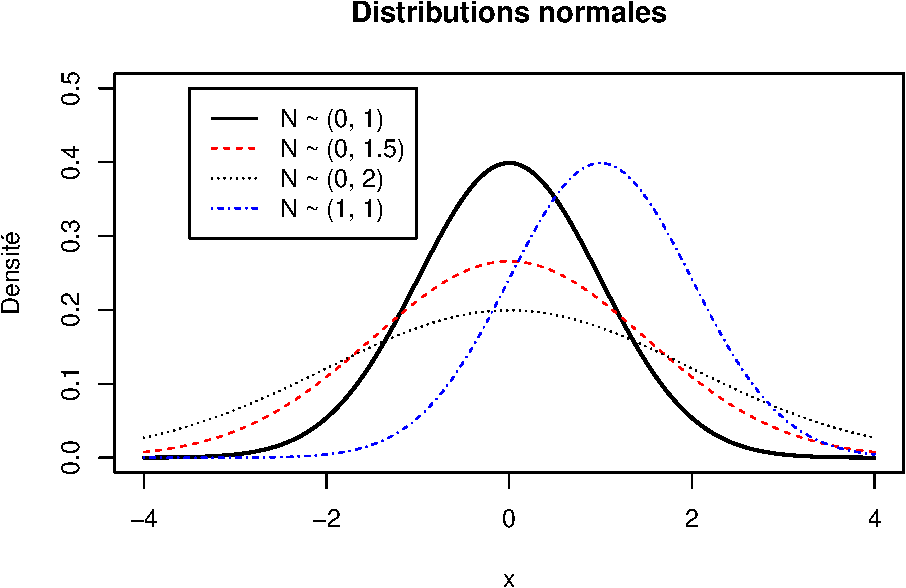
\includegraphics{_main_files/figure-latex/unnamed-chunk-67-1.pdf}

La mesure en unité d'écart-type est standardisée, c'est-à-dire que peu importe l'échelle de mesure originale, la distribution d'une variable peut être ramenée à une échelle mesurée en unité d'écart-type afin de pouvoir adéquatement comparer la distribution d'une variable à une autre variable mesurée différemment\footnote{L'écart-type est calculé par la racine carrée de la moyenne des carrés des écarts entre chaque observation et la moyenne. Soit : \(\sqrt{\frac{\Sigma({x}_{i}-\mu)^2}{N}}\), où \(\chi\) représente une observation \emph{i}, \(\mu\) la moyenne des observations \(\chi_i\) et N Le nombre de cas.}.

Par exemple, la figure suivante montre la distribution de deux variables \(N\sim(\mu, \sigma)\), une variable bleue et une variable rouge. L'échelle en noir est en unités d'écarts-types, alors que les échelles en bleu et en rouge peuvent être pensées comme deux possibilités d'échelles «originales» sur lesquelles les variables ont été mesurées. L'échelle en bleu va de 0 à 80 avec une moyenne de 40, celle en rouge de 40 à 160 avec une moyenne de 100 (on peut par exemple songer à la mesure du QI qui a aussi une moyenne de 100 et un écart-type de 15). Mais lorsque ces échelles sont ramenées en unité d'écarts-types, elles peuvent alors être adéquatement comparées. On remarque qu'en plaçant les échelles originales sur une échelle comparable, leur distribution est identique.

La raison tient à l'une des propriétés fondamentales de la loi normale : pour toute combinaison de moyenne et d'écart-type, il y aura toujours une proportion constante de cas entre la moyenne et un point quelconque situé à une certaine distance de la moyenne exprimée en écart-type. En observant la figure, on pourrait donc dire que, dans le cas de l'échelle bleue, il y a 95.4\% des cas qui se situent entre 20 et 60, alors que 95\% des cas se situent entre 85 et 115 dans le cas de la variable rouge.

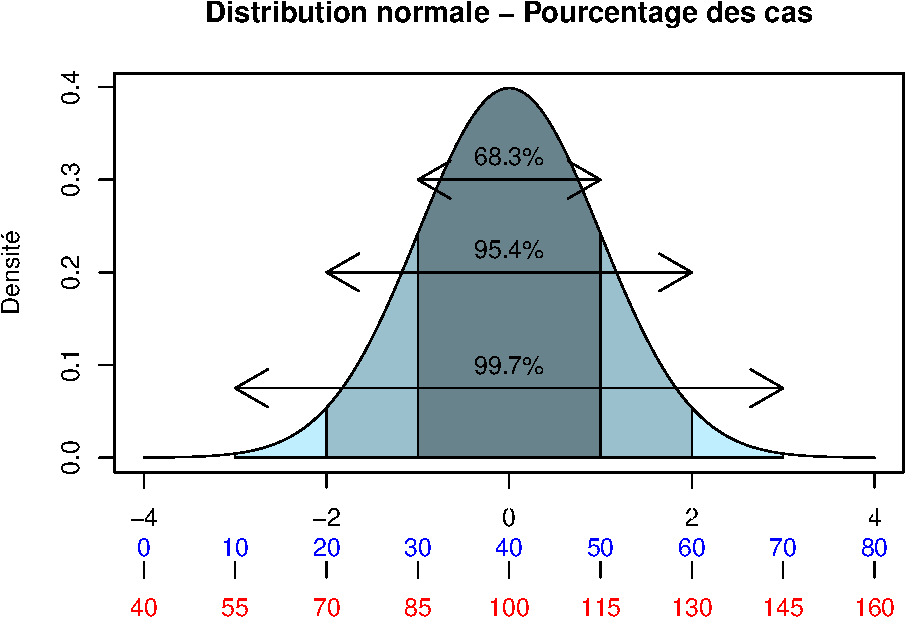
\includegraphics{_main_files/figure-latex/unnamed-chunk-68-1.pdf}

Nous savons qu'il y aura toujours exactement 68.3\% des cas situés à \(\pm 1\sigma\) (plus ou moins 1 écart-type). Il y aura aussi toujours 95.4\% des cas situés à \(\pm 2\sigma\) et 99.7\% des cas situés à \(\pm3\sigma\). Cela sera vrai peu importe l'échelle de mesure originale utilisée pour mesurer une variable.

Cette propriété est vraie pour la distribution illustrée ici, mais elle le serait tout autant pour une distribution qui aurait une apparence plus aplatie. On pourrait «aplatir» la distribution de la figure, mais l'échelle des écarts-types bougerait avec elle. Imaginez que, pour aplatir la distribution, vous tiriez de chaque côté de l'axe des abscisses (x), cela aurait pour effet d'étirer chaque côté de la distribution et donc de l'aplatir, mais l'échelle suivrait elle aussi.

\hypertarget{le-thuxe9oruxe8me-de-la-limite-centrale}{%
\subsection{Le théorème de la limite centrale}\label{le-thuxe9oruxe8me-de-la-limite-centrale}}

Nous venons de voir rapidement l'importance de la distribution normale, mais pour comprendre l'inférence statistique, il est important de saisir qu'il existe trois types de distributions.

\begin{enumerate}
\def\labelenumi{\arabic{enumi}.}
\tightlist
\item
  La distribution d'une population (N)

  \begin{itemize}
  \tightlist
  \item
    Lors d'un rescencement
  \item
    Avec une moyenne \(\mu\) et un écart-type \(\sigma\)
  \end{itemize}
\item
  La distribution d'un échantillon (n)

  \begin{itemize}
  \tightlist
  \item
    Lors d'un sondage
  \item
    Avec une moyenne \(\bar{x}\) (prononcé «x-barre») et un écart-type \(s\)
  \end{itemize}
\item
  La distribution de \emph{tous les échantillons possibles} (distribution d'échantillonnage)

  \begin{itemize}
  \tightlist
  \item
    Toutes les combinaisons possibles des cas qu'il est possible de tirer pour produire un échantillon \emph{n} d'une population \emph{N}.
  \end{itemize}
\end{enumerate}

Les deux premiers types de distributions sont relativement intuitifs, le troisième est cependant plus difficile à saisir. Imaginons la population formée des éléments A, B, C, D, E (\emph{N}=5) et que nous voulions tirer un échantillon de taille 2 (\emph{n}=2). Dans ce cas, tous les échantillons possibles correspondent à toutes les paires de lettres qu'il est possible de tirer à partir de la population. Dans notre cas, il a a 10 échantillons possibles : AB, AC, AD, AE, BC, BD, BE, CD, CE et DE. Le nombre total d'échantillons possibles peut être calculé à partir du NcN :

\[Ncn=\frac{N!}{ n!(N-n)! }\]
Le signe ! signifie «factoriel», il c'est-à-dire que nous multiplions entre eux la suite de nombre qui vient avec le premier nombre jusqu'à arriver à 1. Dans notre exemple, cela donne:
\[\frac { 5! }{ 2!(5-2)! } =\frac { 5\times 4\times 3\times 2\times 1 }{ 2\times 1\quad (3\times 2\times 1) } =\frac { 120 }{ 12 } =10\]

Dans notre exemple, il y a donc 10 échantillons possibles de 2 lettres dans notre population de 5 lettres. Imaginons maintenant une situation habituelle avec un sondage de 1000 répondants (n=1000) pour une population de 5 millions d'électeurs (N=5 000 000). Tous les échantillons possibles signifient alors toutes les possibilités d'échantillons de \emph{n}=1000 qu'il est possible de tirer d'une population de 5 millions d'individus. Deux échantillons ne différant que par 1 seul individu sont ici considérés comme deux échantillons possibles distincts. Dans ce cas, le nombre d'échantillons possibles donne :
\[Ncn=\frac { N! }{ n!(N-n)! }\]
\[Ncn=\frac { 5 000 000! }{ 1000!(5 000 000-1000)! }\]
\[Ncn = 27 000 000 000 000 000 000 000 000 000 000 000 000 000\]
Le nombre d'échantillons possibles est tellement gros que nous ne savons même pas comment au juste nous devrions dire ce nombre. Vous comprenez donc que cette idée de «tous les échantillons possibles» n'est que \emph{théorique} et ne peut jamais réellement être appliquée. Cependant, sans pour autant que nous fassions la démonstration mathématique, sachez simplement que le théorème de la limite centrale nous apprend qu'au fur et à mesure que \emph{le nombre d'échantillons augmente}, la moyenne d'une variété de paramètres de ces échantillons se rapprochera de plus en plus de la «vraie» valeur des paramètres dans la population.

Attention ici, nous ne parlons pas de la moyenne d'une variable \emph{dans} un échantillon, mais de la \emph{moyenne de la moyenne des échantillons}. Si par exemple nous nous intéressons à la taille moyenne des femmes d'une population donnée, nous prenons un premier échantillon de 100 femmes et nous obtenons une moyenne de 167cm. Nous prenons ensuite un second échantillon et nous obtenons une moyenne de 172cm. Un troisième échantillon nous donne une moyenne de 169 cm. À mesure que nous augmentons le nombre d'échantillons, la moyenne de ceux-ci (ici, la moyenne de 167, 172 et 169), qui revient à la moyenne des moyennes \emph{dans} les échantillons\_ se rapprochera de plus en plus de la «vraie» valeur dans la population. Mathématiquement, il pourrait être démontré que la moyenne de tous les échantillons possibles (la «moyenne échantillonnale») est égale à la moyenne de la population. Par ailleurs, la \emph{disrtribution} de ces moyennes d'échantillons tendra à devenir normale et cela sera d'autant plus vrai que la taille des échantillons individuels sera grande.

Si la taille de l'échantillon est de 30 ou plus, les trois choses suivantes seront vraies :
- La moyenne de la distribution d'échantillonnage est identique à la moyenne de la population (\({ \mu }_{ \bar{x} }\)=\(\mu\))
- La distribution d'échantillonnage suit une distribution normale.
- Son écart-type sera de \(\frac { \sigma }{ \sqrt { N } }\)

\hypertarget{luxe9chantillonnage}{%
\section{L'échantillonnage}\label{luxe9chantillonnage}}

Afin d'illustrer le théorème de la limite centrale, qui est plus facile à saisir en le «voyant» à l'oeuvre qu'en tentant de le comprendre abstraitement, nous allons simuler des données d'une population de 10 millions de personnes et allons ensuite faire des «sondages» aléatoires dans cette population. Nous utiliserons deux scénarios. D'abord une élection entre deux partis, l'un étant réellement à 55\% et l'autre à 45\% d'intentions de vote dans la population. Puis nous simulerons une situation où la course entre ces deux partis est serrée, l'un étant réellement à 51\% et l'autre à 49\%. Nous observerons ce qui se produit lorsque nous augmentons la quantité de «sondages», et aussi de quoi ont l'air ces sondages lorsque le véritable écart entre les deux partis est relativement petit.

\hypertarget{exemple-dune-uxe9lection-uxe0-deux-partis-55-45}{%
\subsection{Exemple d'une élection à deux partis (55-45)}\label{exemple-dune-uxe9lection-uxe0-deux-partis-55-45}}

Nous simulons d'abord les données de la population de 10 millions d'individus

\begin{Shaded}
\begin{Highlighting}[]
\CommentTok{\# Créons les données de la population entière de 10M d\textquotesingle{}électeurs.}
\NormalTok{population }\OtherTok{\textless{}{-}} \FunctionTok{sample}\NormalTok{(}\FunctionTok{c}\NormalTok{(}\DecValTok{1}\NormalTok{, }\DecValTok{0}\NormalTok{), }\AttributeTok{size=}\DecValTok{10000000}\NormalTok{, }\AttributeTok{rep=}\ConstantTok{TRUE}\NormalTok{, }\AttributeTok{prob=}\FunctionTok{c}\NormalTok{(.}\DecValTok{55}\NormalTok{,.}\DecValTok{45}\NormalTok{))}
\CommentTok{\# L\textquotesingle{}objet population contient donc 5 millions de lignes (individus) qui votent }
\CommentTok{\# pour les différents partis dans les proportions décrites.}

\FunctionTok{ftable}\NormalTok{(population) }\CommentTok{\# Voir le nombre d\textquotesingle{}individus qui votent pour chaque parti.}
\end{Highlighting}
\end{Shaded}

\begin{verbatim}
## population       0       1
##                           
##            4499648 5500352
\end{verbatim}

\begin{Shaded}
\begin{Highlighting}[]
\CommentTok{\# Bien sûr, les proportions seraient plus informatives. Demandons{-}les à R. }
\FunctionTok{prop.table}\NormalTok{(}\FunctionTok{table}\NormalTok{(population)) }\CommentTok{\# Pour en voir les proportions}
\end{Highlighting}
\end{Shaded}

\begin{verbatim}
## population
##         0         1 
## 0.4499648 0.5500352
\end{verbatim}

Nous voyons donc qu'il y a effectivement 55.00352\% des gens qui ont l'entention de voter pour le parti bleu et 44.99648\% qui ont l'intention de voter pour le parti rouge. Ce sont ici les \emph{vraies} intentions de vote dans notre \emph{population}. Imaginons maintenant que nous fassions un sondage aléatoire de 1000 individus dans cette population.

\begin{Shaded}
\begin{Highlighting}[]
\CommentTok{\# Faisons un premier sondage aléatoire de cette population }
\CommentTok{\# avec un échantillon de 1000 personnes.}
\NormalTok{sondage}\FloatTok{.1} \OtherTok{\textless{}{-}} \FunctionTok{sample}\NormalTok{(population, }\DecValTok{1000}\NormalTok{, }\AttributeTok{replace=}\ConstantTok{FALSE}\NormalTok{)}
\FunctionTok{prop.table}\NormalTok{(}\FunctionTok{table}\NormalTok{(sondage}\FloatTok{.1}\NormalTok{))}
\end{Highlighting}
\end{Shaded}

\begin{verbatim}
## sondage.1
##     0     1 
## 0.473 0.527
\end{verbatim}

Nous obtenons ici qu'une proportion de 0.527 des «répondants» affirment vouloir voter pour le parti bleu et 0.473 pour le parti rouge. Faisons un deuxième sondage aléatoire.

\begin{Shaded}
\begin{Highlighting}[]
\CommentTok{\# Un deuxième sondage}
\NormalTok{sondage}\FloatTok{.2} \OtherTok{\textless{}{-}} \FunctionTok{sample}\NormalTok{(population, }\DecValTok{1000}\NormalTok{, }\AttributeTok{replace=}\ConstantTok{FALSE}\NormalTok{)}
\FunctionTok{prop.table}\NormalTok{(}\FunctionTok{table}\NormalTok{(sondage}\FloatTok{.2}\NormalTok{))}
\end{Highlighting}
\end{Shaded}

\begin{verbatim}
## sondage.2
##     0     1 
## 0.444 0.556
\end{verbatim}

Nous obtenons 55.6\% pour le parti bleu et 44.4\% pour le parti rouge. Faisons un troisième sondage.

\begin{Shaded}
\begin{Highlighting}[]
\CommentTok{\# Un troisième sondage}
\NormalTok{sondage}\FloatTok{.3} \OtherTok{\textless{}{-}} \FunctionTok{sample}\NormalTok{(population, }\DecValTok{1000}\NormalTok{, }\AttributeTok{replace=}\ConstantTok{FALSE}\NormalTok{)}
\FunctionTok{prop.table}\NormalTok{(}\FunctionTok{table}\NormalTok{(sondage}\FloatTok{.3}\NormalTok{))}
\end{Highlighting}
\end{Shaded}

\begin{verbatim}
## sondage.3
##     0     1 
## 0.475 0.525
\end{verbatim}

Ici, nous obtenons que 52.5\% des répondants affirment vouloir voter pour le parti bleu, alors que 47.5 disent vouloir voter pour le parti rouge. Tentons un quatrième sondage.

\begin{Shaded}
\begin{Highlighting}[]
\CommentTok{\# Un quatrième sondage}
\NormalTok{sondage}\FloatTok{.4} \OtherTok{\textless{}{-}} \FunctionTok{sample}\NormalTok{(population, }\DecValTok{1000}\NormalTok{, }\AttributeTok{replace=}\ConstantTok{FALSE}\NormalTok{)}
\FunctionTok{prop.table}\NormalTok{(}\FunctionTok{table}\NormalTok{(sondage}\FloatTok{.4}\NormalTok{))}
\end{Highlighting}
\end{Shaded}

\begin{verbatim}
## sondage.4
##     0     1 
## 0.441 0.559
\end{verbatim}

Avec ce quatrième sondage, nous obtenons que 55.9\% des répondants affirment vouloir voter pour le parti bleu, alors que 44.1. Essayons un dernier sondage.

\begin{Shaded}
\begin{Highlighting}[]
\CommentTok{\# Un cinquième sondage}
\NormalTok{sondage}\FloatTok{.5} \OtherTok{\textless{}{-}} \FunctionTok{sample}\NormalTok{(population, }\DecValTok{1000}\NormalTok{, }\AttributeTok{replace=}\ConstantTok{FALSE}\NormalTok{)}
\FunctionTok{prop.table}\NormalTok{(}\FunctionTok{table}\NormalTok{(sondage}\FloatTok{.5}\NormalTok{))}
\end{Highlighting}
\end{Shaded}

\begin{verbatim}
## sondage.5
##     0     1 
## 0.457 0.543
\end{verbatim}

Avec ce cinquième sondage, nous obtenons que 54.3\% des répondants affirment vouloir voter pour le parti bleu, alors que 45.7.

Nous pourrions continuer ainsi à faire des sondages, mais remarquez deux choses : les résultats de chaque sondage ne sont par forcément «pile» sur les «vrais» chiffres dans la population (55\% pour les bleus et 45\% pour les rouges), mais ils tournent globalement autour de ceux-ci. Aussi, si nous faisons la moyenne des résultats obtenus dans ces cinq sondages, nous obtiendrions un résultat qui se rapprocherait encore plus de la vraie valeur. Essayons-le.

\begin{Shaded}
\begin{Highlighting}[]
\CommentTok{\# Moyenne des résultats des 5 sondages pour le parti bleu}
\FunctionTok{mean}\NormalTok{(}\FunctionTok{prop.table}\NormalTok{(}\FunctionTok{table}\NormalTok{(sondage}\FloatTok{.1}\NormalTok{))[}\DecValTok{2}\NormalTok{],}
     \FunctionTok{prop.table}\NormalTok{(}\FunctionTok{table}\NormalTok{(sondage}\FloatTok{.2}\NormalTok{))[}\DecValTok{2}\NormalTok{],}
     \FunctionTok{prop.table}\NormalTok{(}\FunctionTok{table}\NormalTok{(sondage}\FloatTok{.3}\NormalTok{))[}\DecValTok{2}\NormalTok{],}
     \FunctionTok{prop.table}\NormalTok{(}\FunctionTok{table}\NormalTok{(sondage}\FloatTok{.4}\NormalTok{))[}\DecValTok{2}\NormalTok{],}
     \FunctionTok{prop.table}\NormalTok{(}\FunctionTok{table}\NormalTok{(sondage}\FloatTok{.5}\NormalTok{))[}\DecValTok{2}\NormalTok{]}
\NormalTok{     )}
\end{Highlighting}
\end{Shaded}

\begin{verbatim}
## [1] 0.527
\end{verbatim}

\begin{Shaded}
\begin{Highlighting}[]
\CommentTok{\# Moyenne des résultats des 5 sondages pour le parti rouge}
\FunctionTok{mean}\NormalTok{(}\FunctionTok{prop.table}\NormalTok{(}\FunctionTok{table}\NormalTok{(sondage}\FloatTok{.1}\NormalTok{))[}\DecValTok{1}\NormalTok{],}
     \FunctionTok{prop.table}\NormalTok{(}\FunctionTok{table}\NormalTok{(sondage}\FloatTok{.2}\NormalTok{))[}\DecValTok{1}\NormalTok{],}
     \FunctionTok{prop.table}\NormalTok{(}\FunctionTok{table}\NormalTok{(sondage}\FloatTok{.3}\NormalTok{))[}\DecValTok{1}\NormalTok{],}
     \FunctionTok{prop.table}\NormalTok{(}\FunctionTok{table}\NormalTok{(sondage}\FloatTok{.4}\NormalTok{))[}\DecValTok{1}\NormalTok{],}
     \FunctionTok{prop.table}\NormalTok{(}\FunctionTok{table}\NormalTok{(sondage}\FloatTok{.5}\NormalTok{))[}\DecValTok{1}\NormalTok{]}
\NormalTok{     )}
\end{Highlighting}
\end{Shaded}

\begin{verbatim}
## [1] 0.473
\end{verbatim}

Nous n'avons que cinq sondages et notre moyenne n'est donc pas pile sur les vrais résultats de la population, mais nous nous en approchons beaucoup. Imaginons que nous fassions 50 sondages plutôt que seulement 5.

\begin{Shaded}
\begin{Highlighting}[]
\NormalTok{data.sondages }\OtherTok{\textless{}{-}} \FunctionTok{list}\NormalTok{()}
\ControlFlowTok{for}\NormalTok{(i }\ControlFlowTok{in} \DecValTok{1}\SpecialCharTok{:}\DecValTok{50}\NormalTok{)\{ }\CommentTok{\# Ceci est un "loop", nous faisons la même commande 50 fois}
\NormalTok{    data.sondages[[i]] }\OtherTok{\textless{}{-}} \FunctionTok{sample}\NormalTok{(population, }\DecValTok{1000}\NormalTok{, }\AttributeTok{replace=}\ConstantTok{FALSE}\NormalTok{)}
\NormalTok{\}}

\NormalTok{prop.sondages }\OtherTok{=} \FunctionTok{vector}\NormalTok{()}
\ControlFlowTok{for}\NormalTok{(i }\ControlFlowTok{in} \DecValTok{1} \SpecialCharTok{:}\DecValTok{50}\NormalTok{)\{}
\NormalTok{    prop.sondages[i] }\OtherTok{\textless{}{-}} \FunctionTok{mean}\NormalTok{(data.sondages[[i]])}
\NormalTok{\}}
\FunctionTok{mean}\NormalTok{(prop.sondages)}
\end{Highlighting}
\end{Shaded}

\begin{verbatim}
## [1] 0.55378
\end{verbatim}

On pourrait difficilement faire mieux. Ceci dit, ici notre exemple posait que les vraies valeurs étaient à 55\% et 45\%, soit une différence de 10 points de pourcentage entre les deux partis. Dans la réalité, il arrive souvent que les vraies intentions de vote soient beaucoup plus serrées. Imaginons donc que nous une course très serrée dans laquelle le parti Bleu ne mène que par 2 points de pourcentage.

\hypertarget{exemple-dune-uxe9lection-serruxe9e-51-49}{%
\subsection{Exemple d'une élection serrée (51-49)}\label{exemple-dune-uxe9lection-serruxe9e-51-49}}

\begin{Shaded}
\begin{Highlighting}[]
\CommentTok{\# Créons les données de la population entière de 10M d\textquotesingle{}électeurs.}
\NormalTok{population.serre }\OtherTok{\textless{}{-}} \FunctionTok{sample}\NormalTok{(}\FunctionTok{c}\NormalTok{(}\DecValTok{1}\NormalTok{, }\DecValTok{0}\NormalTok{), }\AttributeTok{size=}\DecValTok{10000000}\NormalTok{, }\AttributeTok{rep=}\ConstantTok{TRUE}\NormalTok{, }\AttributeTok{prob=}\FunctionTok{c}\NormalTok{(.}\DecValTok{51}\NormalTok{,.}\DecValTok{49}\NormalTok{))}
\CommentTok{\# L\textquotesingle{}objet population contient donc 5 millions de lignes (individus) qui votent }
\CommentTok{\# pour les différents partis dans les proportions décrites.}

\FunctionTok{prop.table}\NormalTok{(}\FunctionTok{table}\NormalTok{(population)) }\CommentTok{\# Pour en voir les proportions}
\end{Highlighting}
\end{Shaded}

\begin{verbatim}
## population
##         0         1 
## 0.4499648 0.5500352
\end{verbatim}

Faisons 50 sondages.

\begin{Shaded}
\begin{Highlighting}[]
\NormalTok{data.sondages\_serre }\OtherTok{\textless{}{-}} \FunctionTok{list}\NormalTok{()}
\ControlFlowTok{for}\NormalTok{(i }\ControlFlowTok{in} \DecValTok{1}\SpecialCharTok{:}\DecValTok{50}\NormalTok{)\{ }\CommentTok{\# Ceci est un "loop", même commande 50 fois i=1:50}
\NormalTok{    data.sondages\_serre[[i]] }\OtherTok{\textless{}{-}} \FunctionTok{sample}\NormalTok{(population.serre, }\DecValTok{1000}\NormalTok{, }\AttributeTok{replace=}\ConstantTok{FALSE}\NormalTok{)}
\NormalTok{\}}

\NormalTok{prop.sondages\_serre }\OtherTok{=} \FunctionTok{vector}\NormalTok{()}
\ControlFlowTok{for}\NormalTok{(i }\ControlFlowTok{in} \DecValTok{1} \SpecialCharTok{:}\DecValTok{50}\NormalTok{)\{}
\NormalTok{    prop.sondages\_serre[i] }\OtherTok{\textless{}{-}} \FunctionTok{mean}\NormalTok{(data.sondages\_serre[[i]])}
\NormalTok{\}}
\FunctionTok{mean}\NormalTok{(prop.sondages\_serre)}
\end{Highlighting}
\end{Shaded}

\begin{verbatim}
## [1] 0.512
\end{verbatim}

Vous voyez que nous obtenons une moyenne de nos 50 sondages qui ressemble à ce qui devrait être la vraie valeur de 0.51 pour le parti Bleu. Ceci étant, tous nos sondages n'ont pas, individuellement la même moyenne. Visualisons la distribution de nos sondages pour voir comment se sont répartis les résultats de tous les sondages.

\begin{Shaded}
\begin{Highlighting}[]
\NormalTok{densite\_50 }\OtherTok{\textless{}{-}} \FunctionTok{density}\NormalTok{(prop.sondages\_serre)}

\FunctionTok{plot}\NormalTok{(densite\_50, }
     \AttributeTok{main=}\StringTok{"Distribution des résultats de 50 sondages"}\NormalTok{,}
     \AttributeTok{ylab=}\StringTok{"Fréquence"}\NormalTok{,}
     \AttributeTok{xlab=}\StringTok{"Proportion du vote du parti Bleu"}\NormalTok{)}
\end{Highlighting}
\end{Shaded}

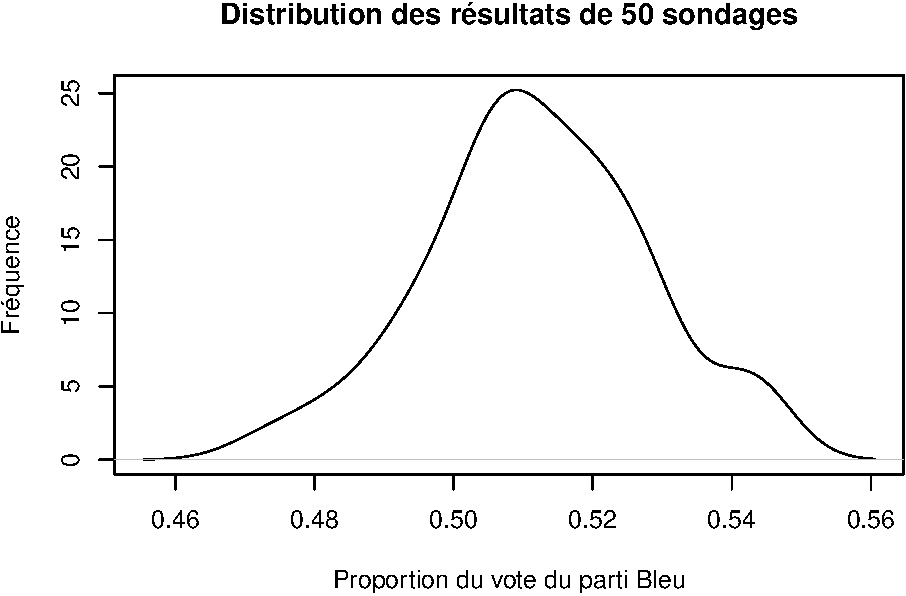
\includegraphics{_main_files/figure-latex/unnamed-chunk-80-1.pdf}

Nous voyons que la distribution des résultats est presque normale, mais pas complètement. La plupart des sondages sont autour de la vraie valeur de 0.51, mais certains en sont plus éloignés. Imaginons maintenant que nous fassions 500 sondages plutôt que 50. Voyons voir.

\begin{Shaded}
\begin{Highlighting}[]
\NormalTok{data.sondages\_serre\_500 }\OtherTok{\textless{}{-}} \FunctionTok{list}\NormalTok{()}
\ControlFlowTok{for}\NormalTok{(i }\ControlFlowTok{in} \DecValTok{1}\SpecialCharTok{:}\DecValTok{500}\NormalTok{)\{}
\NormalTok{    data.sondages\_serre\_500[[i]] }\OtherTok{\textless{}{-}} \FunctionTok{sample}\NormalTok{(population.serre, }\DecValTok{1000}\NormalTok{, }\AttributeTok{replace=}\ConstantTok{FALSE}\NormalTok{)}
\NormalTok{\}}

\NormalTok{prop.sondages\_serre\_500 }\OtherTok{=} \FunctionTok{vector}\NormalTok{()}
\ControlFlowTok{for}\NormalTok{(i }\ControlFlowTok{in} \DecValTok{1}\SpecialCharTok{:}\DecValTok{500}\NormalTok{)\{}
\NormalTok{    prop.sondages\_serre\_500[i] }\OtherTok{\textless{}{-}} \FunctionTok{mean}\NormalTok{(data.sondages\_serre\_500[[i]])}
\NormalTok{\}}
\FunctionTok{mean}\NormalTok{(prop.sondages\_serre\_500)}
\end{Highlighting}
\end{Shaded}

\begin{verbatim}
## [1] 0.509358
\end{verbatim}

Encore une fois, vous voyez que nous obtenons une moyenne très près de ce qui devrait être la vraie valeur de 0.51 pour le parti Bleu. Visualisons encore la distribution pour voir comment se sont répartis les résultats de tous les sondages.

\begin{Shaded}
\begin{Highlighting}[]
\NormalTok{densite\_500 }\OtherTok{\textless{}{-}} \FunctionTok{density}\NormalTok{(prop.sondages\_serre\_500)}

\FunctionTok{plot}\NormalTok{(densite\_500, }
     \AttributeTok{main=}\StringTok{"Distribution des résultats de 500 sondages"}\NormalTok{,}
     \AttributeTok{ylab=}\StringTok{"Fréquence"}\NormalTok{,}
     \AttributeTok{xlab=}\StringTok{"Proportion du vote du parti Bleu"}\NormalTok{)}
\end{Highlighting}
\end{Shaded}

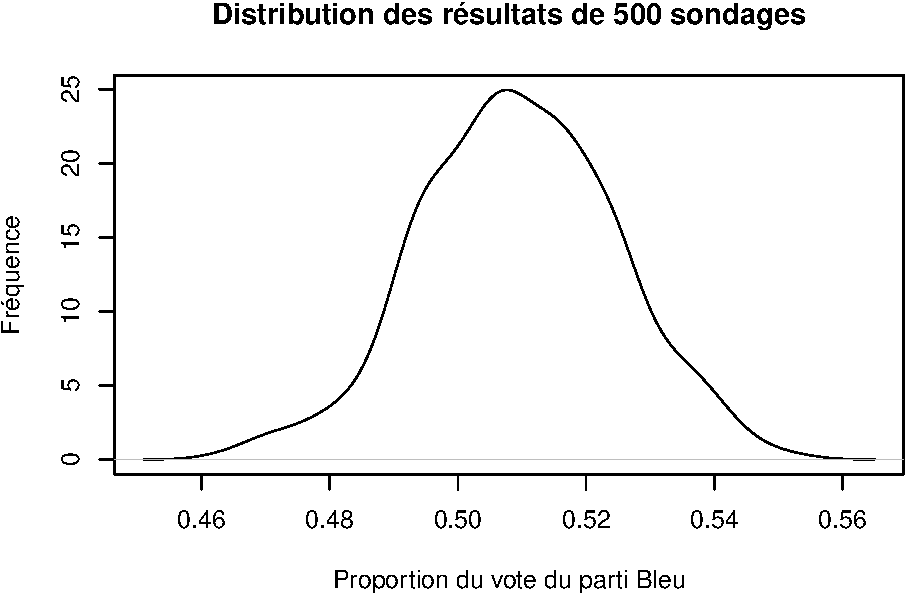
\includegraphics{_main_files/figure-latex/unnamed-chunk-82-1.pdf}

Clairement, cette distribution est beaucoup plus près d'une distribution normale que ce que nous observions avec «seulement» 50 sondages. Essayons avec 5000.

\begin{Shaded}
\begin{Highlighting}[]
\NormalTok{data.sondages\_serre\_5000 }\OtherTok{\textless{}{-}} \FunctionTok{list}\NormalTok{()}
\ControlFlowTok{for}\NormalTok{(i }\ControlFlowTok{in} \DecValTok{1}\SpecialCharTok{:}\DecValTok{5000}\NormalTok{)\{ }
\NormalTok{    data.sondages\_serre\_5000[[i]] }\OtherTok{\textless{}{-}} \FunctionTok{sample}\NormalTok{(population.serre, }\DecValTok{1000}\NormalTok{, }\AttributeTok{replace=}\ConstantTok{FALSE}\NormalTok{)}
\NormalTok{\}}

\NormalTok{prop.sondages\_serre\_5000 }\OtherTok{=} \FunctionTok{vector}\NormalTok{()}
\ControlFlowTok{for}\NormalTok{(i }\ControlFlowTok{in} \DecValTok{1}\SpecialCharTok{:}\DecValTok{5000}\NormalTok{)\{}
\NormalTok{    prop.sondages\_serre\_5000[i] }\OtherTok{\textless{}{-}} \FunctionTok{mean}\NormalTok{(data.sondages\_serre\_5000[[i]])}
\NormalTok{\}}

\NormalTok{densite\_5000 }\OtherTok{\textless{}{-}} \FunctionTok{density}\NormalTok{(prop.sondages\_serre\_5000)}
\FunctionTok{plot}\NormalTok{(densite\_5000, }
     \AttributeTok{main=}\StringTok{"Distribution des résultats de 5000 sondages"}\NormalTok{,}
     \AttributeTok{ylab=}\StringTok{"Fréquence"}\NormalTok{,}
     \AttributeTok{xlab=}\StringTok{"Proportion du vote du parti Bleu"}\NormalTok{)}
\end{Highlighting}
\end{Shaded}

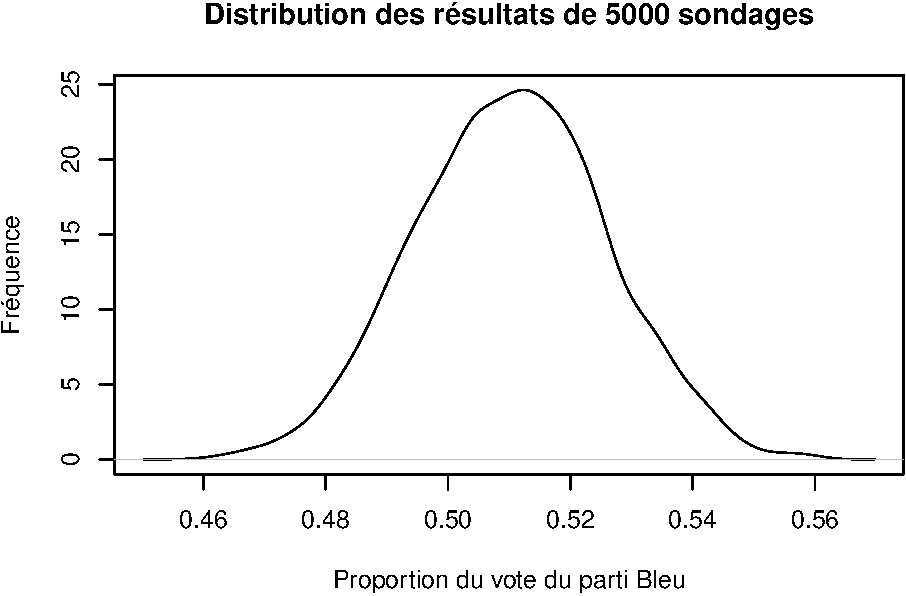
\includegraphics{_main_files/figure-latex/unnamed-chunk-83-1.pdf}

Clairement, la distribution de tous les sondages commence à prendre la forme d'une distribution normale avec une moyenne centrée autour de la vraie valeur de 0.51. Remarquez aussi que quelques sondages s'écartent de cette valeur, il y en a par exemple qui placent le parti Bleu à 0.46 et d'autres à 0.56, mais la très vaste majorité des sondages sont rapprochés de la vraie valeur de 0.51. Remarquez aussi qu'avec une différence de seulement 2 points de pourcentage entre les deux partis (dans la population), il y a quand même une grande quantité de sondages qui donnent moins de 50\% des voix au parti Bleu, même si nous savons que ce dernier devrait être à 51\%. Également, si nous comparons cette distribution avec 5000 sondages avec celle que nous avons obtenu avec 500 sondages, nous voyons aussi que la distribution avec 5000 sondages est plus resserrée, son écart-type est plus faible.

Cette démonstration devrait vous aider à saisir pourquoi il ne faut pas trop s'affoler avec des mouvements de 1, 2 ou 3 points de pourcentages d'un sondage à l'autre. Deux sondages menés la même journée et exactement de la même manière pourront donner des résultats différents. Ces variations inévitables sont le simple fait des aléas de l'échantillonnage statistique. Si l'on prend également en compte que, contrairement à nos 10 millions d'individus fictifs, les vrais citoyens peuvent décider de ne pas répondre (donc l'échantillonnage n'est jamais parfaitement aléatoire parce que la non-réponse peu être plus probable chez certains groupes) et que les maisons de sondage peuvent poser les questions de manière légèrement différente (ce qui peut également entraîner de légères variations dans les résultats), on comprendra qu'il n'y a vraiment pas de quoi écrire à sa mère pour des variations de quelques points de pourcentage.

\hypertarget{du-sondage-uxe0-la-population}{%
\section{Du sondage à la population}\label{du-sondage-uxe0-la-population}}

Évidemment, on ne fait jamais 5000 sondages, ni même 500. La plupart du temps, nous n'avons qu'un seul sondage à partir duquel on veut tirer des inférences sur une population entière. Comme nous l'avons vu, bien que les résultats des sondages tendent à se rapprocher des véritables valeurs d'une population, les aléas de l'échantillonnage font en sorte que les valeurs que nous obtenons dans un sondage donné dévient des vraies valeurs. Ainsi, il est plus prudent de construire une marge d'erreur autour des résultats du sondage.

\hypertarget{la-marge-derreur}{%
\subsection{La marge d'erreur}\label{la-marge-derreur}}

Heureusement, grâce au théorème de la limite centrale, il est possible calculer avec précision un intervalle à l'intérieur duquel le véritable paramètre de la population devrait se retrouver, ce à un degré de confiance désiré. Généralement, le degré de confiance que nous visons est de 95\%, c'est-à-dire que nous acceptons qu'il y ait 5\% des chances que l'on se trompe en affirmant que le véritable paramètre de la population se retrouve à l'intérieur de l'interval que nous aurons calculé. Il convient cependant de remarquer que cette «ligne de démarcation» n'est que conventionnelle et a été fortement contestée récemment (voir notamment \citet{Benjamin2017} et la réponse de \citet{Lakens2018}).

Grâce au théorème de la limite centrale, nous savons que 95\% des échantillons possibles donneront un pourcentage situé à plus ou moins 1.96 écart-types du vrai pourcentge. Nous savons cela grâce à la propriété de la distribution normale discutée plus haut : pour chaque combinaison de moyenne et d'écart-type, il y aura toujours une proportion constante de cas entre la moyenne et un point quelconque situé à une certaine distance de la moyenne exprimée en écart-type. Ici, nous voulons être certain à 95\% de certidue, et donc nous savons que 95\% des cas sont situés à l'intérieur de plus ou moins 1.96 écart-types. La figure suivante illustre la chose pour une distribution échantillonale ayant une moyenne de 0. 95\% de tous les échantillons possibles nous donnerons un résultat situé dans la zone bleue.

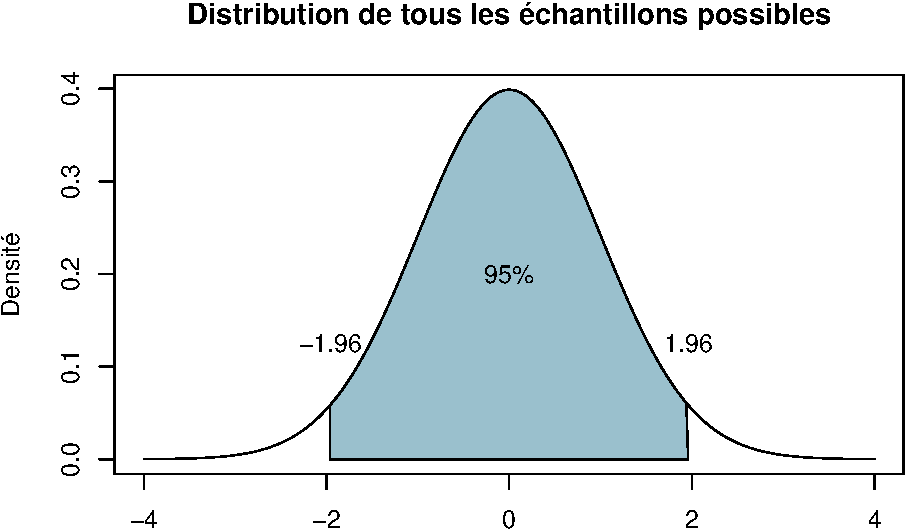
\includegraphics{_main_files/figure-latex/unnamed-chunk-84-1.pdf}

Suivant cela, si nous voulons estimer le pourcentage \(\pi\) d'une population, nous pouvons le faire en utilisant le pourcentage \emph{p} obtenu dans un sondage.\footnote{Les équations pour l'estimation d'une moyenne sont similaires. Il suffit de remplacer les signes appropriés, ce qui donne \(\mu=\bar{x}\pm 1.96 {\sigma}_{\bar{x}}\), où \({\sigma}_{\bar{x}}=\frac{s}{\sqrt{ n }}\)} L'équation suivante permet de calculer la marge d'erreur autour de notre pourcentage \emph{p} à l'intérieur de laquelle nous avons 95\% des chances de trouver le véritable pourcentge \(\pi\) dans la population.

\[\pi=p\pm 1,96 {\sigma}_{p}\]
Où l'écart-type de la distribution échantillonnale \({\sigma}_{p}\) est estimé à partir de l'écart-type \emph{s} dans notre sondage.\\
\[{\sigma}_{p} = \frac { s }{ \sqrt { n }  }\]

\hypertarget{test-de-la-marge-derreur-du-pourcentage-55-45}{%
\subsubsection{Test de la marge d'erreur du pourcentage (55-45)}\label{test-de-la-marge-derreur-du-pourcentage-55-45}}

\begin{Shaded}
\begin{Highlighting}[]
\CommentTok{\# avec un échantillon de 1000 personnes.}
\NormalTok{sondage}\FloatTok{.1} \OtherTok{\textless{}{-}} \FunctionTok{sample}\NormalTok{(population, }\DecValTok{1000}\NormalTok{, }\AttributeTok{replace=}\ConstantTok{FALSE}\NormalTok{)}
\FunctionTok{prop.table}\NormalTok{(}\FunctionTok{table}\NormalTok{(sondage}\FloatTok{.1}\NormalTok{))}
\end{Highlighting}
\end{Shaded}

\begin{verbatim}
## sondage.1
##     0     1 
## 0.424 0.576
\end{verbatim}

\begin{Shaded}
\begin{Highlighting}[]
\CommentTok{\# Pour avoir l\textquotesingle{}écart{-}type}
\FunctionTok{sd}\NormalTok{(sondage}\FloatTok{.1}\NormalTok{) }\CommentTok{\# sd() pour standard deviation}
\end{Highlighting}
\end{Shaded}

\begin{verbatim}
## [1] 0.4944375
\end{verbatim}

\begin{Shaded}
\begin{Highlighting}[]
\CommentTok{\# Calculon Sigma\_p}
\NormalTok{sigma\_p }\OtherTok{\textless{}{-}} \FunctionTok{sd}\NormalTok{(sondage}\FloatTok{.1}\NormalTok{)}\SpecialCharTok{/}\FunctionTok{sqrt}\NormalTok{(}\DecValTok{1000}\NormalTok{)}

\CommentTok{\# Calculons l\textquotesingle{}intervalle de confiance à 95\%}
\NormalTok{low\_bound }\OtherTok{\textless{}{-}} \FunctionTok{mean}\NormalTok{(sondage}\FloatTok{.1}\NormalTok{)}\SpecialCharTok{{-}}\FloatTok{1.96}\SpecialCharTok{*}\NormalTok{sigma\_p}
\NormalTok{low\_bound}
\end{Highlighting}
\end{Shaded}

\begin{verbatim}
## [1] 0.5453544
\end{verbatim}

\begin{Shaded}
\begin{Highlighting}[]
\NormalTok{hi\_bound }\OtherTok{\textless{}{-}} \FunctionTok{mean}\NormalTok{(sondage}\FloatTok{.1}\NormalTok{)}\SpecialCharTok{+}\FloatTok{1.96}\SpecialCharTok{*}\NormalTok{sigma\_p}
\NormalTok{hi\_bound}
\end{Highlighting}
\end{Shaded}

\begin{verbatim}
## [1] 0.6066456
\end{verbatim}

Donc, suivant notre calcul sur un sondage dans lequel le parti bleu avait 56\% des intentions de vote, l'interval bas est de 0.5453544 et l'interval haut de 0.6066456. Suivant notre scénario, nous savons que le pourcentage \(\pi\) réel d'intention de vote dans la population est de 55\%, ce qui est bel et bien à l'intérieur de notre interval de confiance. Évidemment, ici nous avons l'avantage de connaître la véritable valeur du pourcentage de la population puisque nous l'avons nous-mêmes créé, ce n'est évidemment normalement pas le cas.

\hypertarget{test-de-la-marge-derreur-du-pourcentage-51-49}{%
\subsubsection{Test de la marge d'erreur du pourcentage (51-49)}\label{test-de-la-marge-derreur-du-pourcentage-51-49}}

Juste histoire de s'amuser, tentons aussi l'expérience avec notre scénario d'élection serrée.

\begin{Shaded}
\begin{Highlighting}[]
\CommentTok{\# avec un échantillon de 1000 personnes.}
\NormalTok{sondage}\FloatTok{.1}\NormalTok{\_s }\OtherTok{\textless{}{-}} \FunctionTok{sample}\NormalTok{(population.serre, }\DecValTok{1000}\NormalTok{, }\AttributeTok{replace=}\ConstantTok{FALSE}\NormalTok{)}
\FunctionTok{prop.table}\NormalTok{(}\FunctionTok{table}\NormalTok{(sondage}\FloatTok{.1}\NormalTok{\_s))}
\end{Highlighting}
\end{Shaded}

\begin{verbatim}
## sondage.1_s
##     0     1 
## 0.489 0.511
\end{verbatim}

\begin{Shaded}
\begin{Highlighting}[]
\CommentTok{\# Pour avoir l\textquotesingle{}écart{-}type}
\FunctionTok{sd}\NormalTok{(sondage}\FloatTok{.1}\NormalTok{\_s) }\CommentTok{\# sd() pour standard deviation}
\end{Highlighting}
\end{Shaded}

\begin{verbatim}
## [1] 0.5001291
\end{verbatim}

\begin{Shaded}
\begin{Highlighting}[]
\NormalTok{sigma\_p }\OtherTok{\textless{}{-}} \FunctionTok{sd}\NormalTok{(sondage}\FloatTok{.1}\NormalTok{\_s)}\SpecialCharTok{/}\FunctionTok{sqrt}\NormalTok{(}\DecValTok{1000}\NormalTok{)}
\FunctionTok{mean}\NormalTok{(sondage}\FloatTok{.1}\NormalTok{\_s)}
\end{Highlighting}
\end{Shaded}

\begin{verbatim}
## [1] 0.511
\end{verbatim}

\begin{Shaded}
\begin{Highlighting}[]
\CommentTok{\# Calculons l\textquotesingle{}intervalle de confiance à 95\%}
\NormalTok{low\_bound.s }\OtherTok{\textless{}{-}} \FunctionTok{mean}\NormalTok{(sondage}\FloatTok{.1}\NormalTok{\_s)}\SpecialCharTok{{-}}\FloatTok{1.96}\SpecialCharTok{*}\NormalTok{sigma\_p}
\NormalTok{low\_bound.s}
\end{Highlighting}
\end{Shaded}

\begin{verbatim}
## [1] 0.4800017
\end{verbatim}

\begin{Shaded}
\begin{Highlighting}[]
\NormalTok{hi\_bound.s }\OtherTok{\textless{}{-}} \FunctionTok{mean}\NormalTok{(sondage}\FloatTok{.1}\NormalTok{\_s)}\SpecialCharTok{+}\FloatTok{1.96}\SpecialCharTok{*}\NormalTok{sigma\_p}
\NormalTok{hi\_bound.s}
\end{Highlighting}
\end{Shaded}

\begin{verbatim}
## [1] 0.5419983
\end{verbatim}

Ici, suivant notre calcul sur un sondage dans lequel le parti codé 1 avait 51.1 \% des intentions de vote, l'intval bas est de 0.4800017 et l'interval haut de 0.5419983. Encore une fois, la vraie valeur du parti codé 1 est bien dans notre interval. Cependant, on remarque aussi que cet interval inclu la vraie valeur des intentions de vote du parti codé 0. Nous voyons donc que lorsque nous sommes devant une situation où les intentions de votes réelles dans la population sont très serrée, il est statistiquement très difficile d'établir avec confiance qu'un parti est réellement en avant d'un autre avec un seul sondage. la raison n'a ici rien à voir avec la fiabilité des méthodes statistiques elles-mêmes, mais est tout simplement lié à la nature même de la précision d'un échantillon et au fait que la précision requise pour «prédire» adéquatement le gagant d'une élection est beaucoup plus élevée quand une élection est serrée que lorsque'elle ne l'est pas.

\hypertarget{la-diffuxe9rence-entre-deux-groupes-le-test-t}{%
\subsection{\texorpdfstring{La différence entre deux groupes : Le Test \emph{t}}{La différence entre deux groupes : Le Test t}}\label{la-diffuxe9rence-entre-deux-groupes-le-test-t}}

Le test-t est un test qui nous permet de déterminer si une différence observée entre deux groupes dans un échantillon peut être généralisée à l'ensemble de la population. Ici, plutôt que d'établir un intervalle à l'intérieur duquel on devrait raisonnablement s'attendre à trouver un paramètre d'intérêt dans notre population, on cherche plutôt à vérifier si la différence que l'on observe entre nos deux groupes dans le sondage existe bel et bien aussi dans la population. Autrement dit, nous nous intéressons à la \emph{signification statistique} de la différence que nous observons dans l'échantillon.

Dans le cas de l'estimation de l'intervalle de confiance autour d'un pourcentage vu plus haut, nous n'avions pas réellement d'hypothèse à tester. Nous savions que le résultat d'un échantillon ne nous donne qu'une approximation de la valeur du paramètre dans la population et avons donc voulu avoir une approche plus rigoureuse pour estimer cette vraie valeur. Ici cependant, nous observons une différence entre deux groupes et nous voulons savoir si elle existe vraiment dans la population.

Intuitivement, puisque nous observons une différence entre nos deux groupes, nous pourrions dire que notre hypothèse est que les deux groupes doivent réellement être différents dans la population. Donc, mathématiquement :

\[\mu_1 \neq \mu_2\]
Or, il n'y a pas de manière formelle de tester réellement cette hypothèse directement. Par contre, si nous l'inversons en formulant l'hypothèse nulle selon laquelle il n'y a pas de différence entre nos deux groupes, alors nous pouvons tester \emph{l'improbabilité} de \(\mu_1 \neq \mu_2\). Donc, mathématiquement nous cherchons à vérifier si :

\[\mu_1=\mu2 \quad ou \quad  \mu_1-\mu2=0\]
Si, suivant nos données, il est jugé trop \emph{improbable} que \(\mu_1-\mu2=0\) (moins de 5\% des chances), alors inversement il sera crédible de croire que \(\mu_1 \neq \mu_2\).

Poser l'hypothèse nulle de cette manière est utile parce que, suivant notre connaissance de la distribution normale et du théorème de la limite centrale, nous savons de quoi devraient avoir l'air 95\% des échantillons possibles dans une situation ou l'hypothèse nulle est vraie dans la population. Nous savons que les aléas de l'échantillnage produiront de la variation autour de la vraie valeur, mais nous savons de quoi devraient avoir l'air cette variation. En ce sens, si ce que nous observons dans nos données n'est \emph{pas} conforme à ce que nous pourrions raisonnablement nous attendre d'observer dans 95\% des échantillons possibles tirés d'une population où il n'y a \emph{pas} de différence entre les deux groupes, alors nous jugerons crédible qu'il y ait réellement une différence dans la population.

Pour renforcer encore ce point : nous savons que dans une population ou \(mu_1=mu_2\), 95\% des échantillons possibles nous donneront un résultat qui sera dans la zone bleue de la figure de distribution présentée plus haut. Si le résultat que nous observons se trouve à l'extérieur de cette zone bleue, dans les extrémités gauche et droite de la distribution, alors nous jugerons \textbf{qu'il est trop improbable de tomber sur un échantillon qui nous montre une telle différence entre \(\mu_1\) et \(\mu_2\) s'il n'y en a pas dans la population. Nous jugerons alors que l'hypothèse nulle est trop improbable, donc peu crédible, et nous la rejetterons. Nous dirons donc que la différence que nous observons dans notre échantillon est «statistiquement significative»}.

Revenons maintenant au tout premier exemple que nous avons utilisé au tout début à propos des notes de 100 étudiants. Imaginons que ces 100 étudiants soient un échantillon provenant d'une population de 10 000 étudiants ayant complété une épreuve ministérielle. Nous pourrions alors vouloir vérifier si la différence que nous avons observé entre les garçons et les filles était le seul fait de cet échantillon ou si cette différence existe réellement dans la population entière. Nous pourrions alors faire le tests-t.

\begin{Shaded}
\begin{Highlighting}[]
\CommentTok{\# Histoire de se raffraîchire la mémoire}
\FunctionTok{head}\NormalTok{(data)}
\end{Highlighting}
\end{Shaded}

\begin{verbatim}
##      notes   sexe heures.etude fille
## 1 56.36004 garçon     3.429696     0
## 2 70.16088  fille     5.102714     1
## 3 61.71704  fille     4.780638     1
## 4 70.84951 garçon     5.656184     0
## 5 72.49611  fille     3.883307     1
## 6 84.08077 garçon     8.094016     0
\end{verbatim}

\begin{Shaded}
\begin{Highlighting}[]
\CommentTok{\# Différence fille{-}garçon dans les notes?}
\FunctionTok{t.test}\NormalTok{(data}\SpecialCharTok{$}\NormalTok{notes}\SpecialCharTok{\textasciitilde{}}\NormalTok{data}\SpecialCharTok{$}\NormalTok{sexe) }\CommentTok{\# \textasciitilde{} pcq sexe est facteur binaire}
\end{Highlighting}
\end{Shaded}

\begin{verbatim}
## 
##  Welch Two Sample t-test
## 
## data:  data$notes by data$sexe
## t = -5.4541, df = 92.215, p-value = 4.102e-07
## alternative hypothesis: true difference in means between group garçon and group fille is not equal to 0
## 95 percent confidence interval:
##  -14.333948  -6.681456
## sample estimates:
## mean in group garçon  mean in group fille 
##             57.52824             68.03595
\end{verbatim}

\begin{Shaded}
\begin{Highlighting}[]
\CommentTok{\# Différence fille{-}garçon dans le temps d\textquotesingle{}étude?}
\FunctionTok{t.test}\NormalTok{(data}\SpecialCharTok{$}\NormalTok{heures.etude}\SpecialCharTok{\textasciitilde{}}\NormalTok{data}\SpecialCharTok{$}\NormalTok{sexe)}
\end{Highlighting}
\end{Shaded}

\begin{verbatim}
## 
##  Welch Two Sample t-test
## 
## data:  data$heures.etude by data$sexe
## t = -4.9518, df = 90.354, p-value = 3.399e-06
## alternative hypothesis: true difference in means between group garçon and group fille is not equal to 0
## 95 percent confidence interval:
##  -2.2376079 -0.9562823
## sample estimates:
## mean in group garçon  mean in group fille 
##             4.360936             5.957881
\end{verbatim}

Un test-t vérifie l'improbabilité d'une valeur d'un échantillon en faisant l'hypothèse que cette valeur est \emph{tirée d'une population dans laquelle cette valeur est de 0} (hypothèse nulle). La logique est très eaxtement la même lorsque nous évaluons la signification statistique des coefficients en régression linéaire. Visualisons les trois modèles que nous avions fait plus haut.

\begin{Shaded}
\begin{Highlighting}[]
\FunctionTok{summary}\NormalTok{(m1)}
\end{Highlighting}
\end{Shaded}

\begin{verbatim}
## 
## Call:
## lm(formula = notes ~ sexe)
## 
## Residuals:
##      Min       1Q   Median       3Q      Max 
## -20.2474  -7.3035  -0.6993   6.0207  26.5525 
## 
## Coefficients:
##             Estimate Std. Error t value Pr(>|t|)    
## (Intercept)   57.528      1.441  39.933  < 2e-16 ***
## sexefille     10.508      1.925   5.458 3.63e-07 ***
## ---
## Signif. codes:  0 '***' 0.001 '**' 0.01 '*' 0.05 '.' 0.1 ' ' 1
## 
## Residual standard error: 9.556 on 98 degrees of freedom
## Multiple R-squared:  0.2331, Adjusted R-squared:  0.2253 
## F-statistic: 29.79 on 1 and 98 DF,  p-value: 3.627e-07
\end{verbatim}

\begin{Shaded}
\begin{Highlighting}[]
\FunctionTok{summary}\NormalTok{(m2)}
\end{Highlighting}
\end{Shaded}

\begin{verbatim}
## 
## Call:
## lm(formula = notes ~ heures.etude)
## 
## Residuals:
##      Min       1Q   Median       3Q      Max 
## -16.3271  -3.7251  -0.6483   4.1989  16.8874 
## 
## Coefficients:
##              Estimate Std. Error t value Pr(>|t|)    
## (Intercept)    36.981      1.957   18.90   <2e-16 ***
## heures.etude    5.030      0.353   14.25   <2e-16 ***
## ---
## Signif. codes:  0 '***' 0.001 '**' 0.01 '*' 0.05 '.' 0.1 ' ' 1
## 
## Residual standard error: 6.227 on 98 degrees of freedom
## Multiple R-squared:  0.6744, Adjusted R-squared:  0.6711 
## F-statistic:   203 on 1 and 98 DF,  p-value: < 2.2e-16
\end{verbatim}

\begin{Shaded}
\begin{Highlighting}[]
\FunctionTok{summary}\NormalTok{(m3)}
\end{Highlighting}
\end{Shaded}

\begin{verbatim}
## 
## Call:
## lm(formula = notes ~ sexe + heures.etude)
## 
## Residuals:
##      Min       1Q   Median       3Q      Max 
## -13.6705  -4.2615  -0.6981   3.9705  16.0712 
## 
## Coefficients:
##              Estimate Std. Error t value Pr(>|t|)    
## (Intercept)   37.3057     1.9227  19.403   <2e-16 ***
## sexefille      3.1023     1.3758   2.255   0.0264 *  
## heures.etude   4.6372     0.3872  11.977   <2e-16 ***
## ---
## Signif. codes:  0 '***' 0.001 '**' 0.01 '*' 0.05 '.' 0.1 ' ' 1
## 
## Residual standard error: 6.101 on 97 degrees of freedom
## Multiple R-squared:  0.6906, Adjusted R-squared:  0.6843 
## F-statistic: 108.3 on 2 and 97 DF,  p-value: < 2.2e-16
\end{verbatim}

Notez que R nous renvoie une valeur \emph{t}. Un coefficient est jugé significatif s'il est trop peu probale que le coefficient obtenu dans un échantillon soit tiré d'une population dans lequel il a la valeur de 0.

Vous voyez donc que le fait que quelque chose soit «statistiquement significatif» n'est absoluement pas une sorte de sceau magique démontrant la véracité absolu de quelque chose. Il s'agit tout simplement d'un critère conventionnel (95\%) fondé sur l'improbabilité d'observer quelque chose dans un échantillon tiré d'une population dans laquelle nous faisons l'hypothèse que ce que nous pensons observer est faux. Au final, il s'agit donc simplement de savoir si ce que nous décrivons dans notre échantillon est aussi probablement vrai dans la population qui nous intéresse. Que ce soit dans un échantillon ou dans une population, ce n'est pas parce que deux groupes sont différents l'un de l'autre que cette différence est réellement \emph{causée} par l'appartenance de groupe. Le fait que quelque chose soit «statistiquement significatif» veut simplement dire qu'il est très improbable que nous observions un certaine chose dans un échantillon si cela n'est pas aussi vrai dans la population. Au-delà d'établir l'association entre les deux phénomènes dans la population, la signification statistique ne nous dit rien de la causalité à proprement parler. En ce sens, il ne faut jamais interpréter la signification statistique comme établissant un rapport causal.

  \bibliography{bibliography.bib}

\end{document}
